\documentclass[12pt,a4paper]{report}
\usepackage[utf8]{inputenc}
\usepackage[T1]{fontenc}
\usepackage{amsmath}
\usepackage{amsfonts}
\usepackage{amssymb}
\usepackage[left=2.5cm,right=2.5cm,top=2.5cm,bottom=2.5cm]{geometry}
\usepackage{lingmacros}
\usepackage{tree-dvips}
\usepackage{caption}
\usepackage{amsmath}
\usepackage{amsthm}
\usepackage{stmaryrd}
\usepackage{fancyhdr}
\usepackage{amssymb}
\usepackage {boxedminipage}
\usepackage[french]{babel}
\usepackage{graphicx}
\usepackage[explicit]{titlesec}
\usepackage{lmodern}
\usepackage{lipsum}
\usepackage {shadow }
\usepackage{color}
\usepackage{wrapfig}
\usepackage{eurosym}
\usepackage[utf8]{inputenc}
\usepackage[french]{babel}
\usepackage[T1]{fontenc}
\usepackage{frcursive}
\usepackage{amsmath,amsthm,amsfonts,amssymb}
\usepackage[Glenn]{fncychap}
\usepackage{color}
\usepackage[dvipsnames,x11names,svgnames,table]{xcolor}
\usepackage{lipsum}
\usepackage{graphicx}
\usepackage{caption}
\usepackage{hyperref}
\usepackage{enumitem}
\usepackage{listings}
\usepackage{fncychap}
\usepackage[toc]{appendix}
\usepackage[titles]{tocloft}
\usepackage[tikz]{bclogo}
\usepackage[many]{tcolorbox}
\usepackage{varwidth}
% \usepackage[most]{tcolorbox}
\usepackage[]{svg}
\usepackage[absolute,overlay]{textpos}
\usepackage[footnote]{acronym}
\usepackage{longtable}
\usepackage{caption}
\usepackage{subcaption}

\newcommand{\mychapter}[2]{
    
    \chapter*{#2}
    \addcontentsline{toc}{chapter}{#2}
}


\newlength\chapnumb
\setlength\chapnumb{3cm}


 
\titleformat{\chapter}[block] {
  \normalfont\sffamily}{}{0pt} {
    \parbox[b]{\chapnumb}{
      \fontsize{120}{110}\selectfont\thechapter}
      \parbox[b]{\dimexpr\textwidth-\chapnumb\relax}{
        \raggedleft
        \hfill{\LARGE#1}\\
        \rule{\dimexpr\textwidth-\chapnumb\relax}{0.4pt}
  }
}
 
\titleformat{name=\chapter,numberless}[block]
{\normalfont\sffamily}{}{0pt}
{\parbox[b]{\chapnumb}{%
   \mbox{}}%
  \parbox[b]{\dimexpr\textwidth-\chapnumb\relax}{%
    \raggedleft%
    \hfill{\LARGE#1}\\
    \rule{\dimexpr\textwidth-\chapnumb\relax}{0.4pt}}}

\definecolor{mGreen}{rgb}{0,0.6,0}
\definecolor{mGray}{rgb}{0.5,0.5,0.5}
\definecolor{mPurple}{rgb}{0.58,0,0.82}
\definecolor{backgroundColour}{rgb}{0.95,0.95,0.92}

\lstdefinestyle{CStyle}{
    backgroundcolor=\color{backgroundColour},   
    commentstyle=\color{mGreen},
    keywordstyle=\color{magenta},
    numberstyle=\tiny\color{mGray},
    stringstyle=\color{mPurple},
    basicstyle=\footnotesize,
    breakatwhitespace=false,         
    breaklines=true,                 
    captionpos=b,                    
    keepspaces=true,                 
    numbers=left,                    
    numbersep=5pt,                  
    showspaces=false,                
    showstringspaces=false,
    showtabs=false,                  
    tabsize=2,
    language=C
}
    
\setcounter{MaxMatrixCols}{10}
%TCIDATA{OutputFilter=Latex.dll}
%TCIDATA{Version=5.50.0.2953}
%TCIDATA{<META NAME="SaveForMode" CONTENT="1">}
%TCIDATA{BibliographyScheme=Manual}
%TCIDATA{LastRevised=Sunday, June 06, 2021 23:04:09}
%TCIDATA{<META NAME="GraphicsSave" CONTENT="32">}
% \hyphenpenalty 100000
% \exhyphenpenalty 100000

%====================== INFORMATION ET REGLES ======================

%rajouter les numérotation pour les \paragraphe et \subparagraphe
\setcounter{secnumdepth}{4}
\setcounter{tocdepth}{4}

\hypersetup{							% Information sur le document
pdfauthor = {EL karmy Othmane,
			El jazouly Anass},			% Auteurs
pdftitle = {Mémoire de Projet de fin d'annee:
Conception et mise en oeuvre d’un éditeur Graphique pour Kubernetes},			% Titre du document
pdfsubject = {Mémoire de Projet},		% Sujet
pdfkeywords = {Tag1, Tag2, Tag3, ...},	% Mots-clefs
pdfstartview={FitH}}					% ajuste la page à la largueur de l'écran
%pdfcreator = {MikTeX},% Logiciel qui a crée le document
%pdfproducer = {}} % Société avec produit le logiciel


%======================== DEBUT DU DOCUMENT ========================

\begin{document}

%régler l'espacement entre les lignes
\newcommand{\HRule}{\rule{\linewidth}{0.5mm}}


\pagenumbering{Roman}
\newpage
%page de garde
\thispagestyle{empty}

\begin{titlepage}
    \begin{center}
    % Upper part of the page. The '~' is needed because only works if a paragraph has started.
    
    \begin{minipage}[C]{0.5\textwidth}
    \raggedright
    
\includegraphics[height=3cm]{images/logosHeaders/ensias.png}
    \end{minipage}%
    \begin{minipage}[C]{0.5\textwidth}
    \raggedleft
    
\includegraphics[height=3.1cm]{images/logos/SG_ABS.png}
    \end{minipage}
    
    \textsc{\Large }\\[1cm]
    \text{\huge   Mémoire de projet de fin d'études } \\[.2cm]
    \text{\Large Pour l'obtention du Titre} \\ [.2cm]
    \text{\huge   D'Ingénieur d'État en Informatique  }\\[.2cm]
    \text{\Large Filière : }
    \text{\huge   Génie Logiciel}\\[.5cm]
    
    % Title
    \HRule \\[0.4cm]
    
    {\huge \bfseries 
    Développement de nouvelles fonctionnalités pour l'application de Banque à Distance\\ "SG CONNECT"\\[0.4cm] }
    \HRule \\
    \emph{Période de stage : 15/02/2023 - 15/08/2023}\\[3cm]
    
    % Author and supervisor
    % \begin{minipage}{0.4\textwidth}
    % \begin{flushleft} \large
    % \emph{Réalisé par :}\\[0.5 cm]
    % EL JAZOULY \textsc{Anass}\\
    
    % \end{flushleft}
    % \end{minipage}
    % \begin{minipage}{0.4\textwidth}
    % \begin{flushright} \large
    % \emph{Encadré par :} \\[0.5 cm]
    % Pr.BOUNABAT \textsc{Bouchaib} ( ENSIAS )\\
    % Mr.ZAROUAL \textsc{Hicham}\\ ( SG ABS ) 
    
    % \end{flushright}
    % \end{minipage}
    

    \begin{minipage}{0.49\textwidth}
        \vspace{-4mm}
      \begin{flushleft} \large
        \emph{\bfseries Réalisé par :}\\[0.3cm]
        M.EL JAZOULY Anass \\[0.5cm]
        \emph{\bfseries Encadré par :} \\[0.3cm]
        M.BOUNABAT Bouchaib - ENSIAS \\[0.3cm]
        M.ZAROUAL Hicham - SG ABS
      \end{flushleft}
    \end{minipage}
    \begin{minipage}{0.49\textwidth}
      \vspace{-6mm}
      \begin{flushright} \large
        % \begin{flushleft} \large
        \emph{\bfseries Jury:} \\[0.3cm]
        M.NASSAR Mahmoud (Président)\\[0.3cm]
        M.EL HAMLAOUI Mahmoud (Examinateur)\\[0.3cm]
        M.BOUNABAT Bouchaib (Encadrant)\\
        % \end{flushleft}
    
      \end{flushright}
    \end{minipage}\\[1cm]
    \vfill
    % Bottom of the page
    {\large  Année académique 2022/2023}\\
    % \emph{Filière : Génie Logiciel}
\end{center}
\end{titlepage}

%page blanche
\thispagestyle{empty}

\begin{center}
    \mychapter{0}{Dédicaces}

    \textbf{\large À mes très chers parents,}

    Les mots me manquent pour exprimer toute la reconnaissance, la fierté et le profond amour que je porte pour les sacrifices qu'ils ont consentis pour ma réussite. Qu'ils trouvent ici le témoignage de ma reconnaissance, ma gratitude et le respect. Que Dieu leur préserve bonne santé et longue vie.

    \vspace{5mm}

    \textbf{\large À mon frère et ma sœur,}

    Je ne peux m'empêcher de penser à la chance que j'ai de les avoir dans ma vie. Merci d'être toujours là pour moi, de me soutenir, de me faire rire et de me rappeler de ne jamais me prendre trop au sérieux. Vous êtes les meilleurs frère et sœur qu'on puisse avoir.

    \vspace{5mm}

    \textbf{\large À mes amis,}

    Je vous remercie pour tous les moments inoubliables que nous avons passés ensemble. Vous avez été un soutien constant et une source d'inspiration tout au long de mon parcours.

    \vspace{5mm}

    \textbf{\large À tous les membres de l'association des élèves ingénieurs de l'ENSIAS (ADEI ENSIAS),}

    Je tiens à exprimer ma reconnaissance pour votre confiance en moi en me choisissant comme président de l'ADEI ENSIAS, à vous remercier pour votre implication et votre contribution active à la vie de l'ENSIAS. C'est grâce à votre engagement que nous avons réussi à réaliser des projets qui ont eu un impact positif sur la vie étudiante. En particulier à ceux avec qui j'ai travaillé en tant que président, mon cher bureau exécutif, je vous remercie pour votre dévouement et votre travail acharné. Je suis fier de vous avoir comme amis et collègues. Je vous souhaite une bonne continuation et beaucoup de succès dans vos projets futurs.

    \vspace{5mm}

    \textbf{\large À mes professeurs de l'ENSIAS,}

    Je tiens à vous exprimer toute ma gratitude pour votre enseignement, votre encadrement et vos conseils tout au long de mon parcours à l'école. Vos compétences et votre passion ont été une source d'inspiration pour moi et ont joué un rôle déterminant dans ma formation.

    \vspace{10mm}

    \textbf{\large Merci à tous pour votre soutien et votre affection.}

\end{center}
\newpage
\mychapter{0}{Remerciement}

\begin{center}
\vspace{3em}
Je tiens à exprimer ma profonde gratitude et mon respect à toutes les personnes qui m'ont apporté leur soutien tout au long de mon stage de fin d'étude, qui a abouti au développement de nouvelles fonctionnalités pour l'application de Banque à Distance (SG CONNECT).\\[0,2cm]

Je remercie tout particulièrement mon tuteur, Monsieur ZAROUAL Hicham, du groupe Société Générale Africain Business Services, pour son accueil chaleureux, son temps précieux, ses précieuses directives et son suivi de qualité tout au long de mon stage.\\[0,2cm]

Je tiens également à remercier l'ensemble du personnel du groupe Société Générale pour leur générosité en temps et en réponse à mes questions.\\[0,2cm]

Mes sincères remerciements vont également à Monsieur BOUNABAT Bouchaib, mon encadrant académique, pour son orientation fructueuse, son sens de l'écoute, son extrême disponibilité et ses précieux conseils.

Je tiens à exprimer ma gratitude à tout le corps professoral et administratif de notre chère école pour leur soutien et leur encouragement tout au long de mon parcours académique.\\[0,2cm]

Enfin, je remercie les membres du jury pour avoir accepté d'évaluer mon travail. Que tous ceux qui m'ont aidé de près ou de loin à réaliser ce projet trouvent ici l'expression de mon estime et de mes vifs remerciements.\\[0,2cm]

Merci à tous.


\end{center}


\newpage
\mychapter{0}{Résumé}

Le présent document constitue la synthèse du travail réalisé dans le cadre de mon stage de fin d’études effectué au sein de la \textbf{SOCIÉTÉ GÉNÉRALE AFRICAN BUSINESS SERVICES}. Ma mission était de contribuer au développement de nouvelles fonctionnalités pour l'application \textbf{SG CONNECT}, qui offre des fonctionnalités bancaires mobiles et web à forte valeur ajoutée pour les clients de la Société Générale de la zone AFS.\\

En intégrant l'équipe Bank Up, en tant qu'un développeur front-end, ma mission était de participer à toutes les étapes nécessaires pour les développements et les déploiements de ces nouvelles fonctionnalités.\\

L'application \textbf{SG CONNECT} est une application web et mobile qui permet aux clients de la banque Société Générale de consulter en temps réel le solde de leurs comptes, l'historique de leurs transactions, d'effectuer des virements nationaux de compte à compte ou vers des bénéficiaires, des retraits sans carte, des transferts d'argent vers le wallet YUP, de paramétrer des alertes, de retrouver une agence ou un distributeur de billets, de télécharger leur RIB et de consulter les cours des devises...\\

Les étapes de la réalisation du projet ont consisté en la mise en place d'une architecture monorepo pour faciliter la gestion du code source, l'ajout de nouvelles fonctionnalités en se basant sur les spécifications techniques fournies, ainsi que l'amélioration de l'expérience utilisateur.\\

La méthodologie Agile Scrum a été adoptée pour mener à bien ce projet, avec une itération toutes les deux semaines, des sprints de développement et des revues de code régulières pour assurer la qualité du code. Ensuite, l'élaboration des maquettes et le développement des User Stories. Nous avons également mis en place des tests unitaires et des tests d'intégration pour garantir le bon fonctionnement de l'application. Les outils utilisés pour le développement incluaient ReactJS, React Native, Nginx, Cypress, Jira et Git.
\vfill

\begin{center}
	\HRule \\
\end{center}

\textbf{Mots clés :} Digital Banking, Monorepo, ReactJs, React Native, UML, JIRA, UX/UI design, Méthodologie Agile, Développement web et Mobile.\\
\begin{center}
	\HRule 
\end{center}
\newpage
\mychapter{0}{Abstract}
The present document constitutes the summary of the work carried out during my end-of-studies internship at \textbf{SOCIÉTÉ GÉNÉRALE AFRICAN BUSINESS SERVICES}. My mission was to contribute to the development of new features for the \textbf{SG CONNECT} application, which offers high-value mobile and web banking functionalities for Société Générale's clients in the AFS region.\\

As a front-end developer, I joined the Bank Up team and participated in all the necessary steps for the development and deployment of these new features.\\

The \textbf{SG CONNECT} application is a web and mobile application that allows Société Générale's clients to check their account balance and transaction history in real-time, make national transfers between accounts or to beneficiaries, perform cardless withdrawals, transfer money to the YUP wallet, set up alerts, find branches or ATMs, download their bank statement, and check currency exchange rates.\\

The project implementation steps included setting up a monorepo architecture to facilitate source code management, adding new features based on provided technical specifications, and enhancing the user experience.\\

The Agile Scrum methodology was adopted to successfully carry out this project, with iterations every two weeks, development sprints, and regular code reviews to ensure code quality. Additionally, wireframe design and User Story development were carried out. We also implemented unit tests and integration tests to ensure the proper functioning of the application. The development tools used included ReactJS, React Native, Nginx, Cypress, Jira, and Git.

\vfill

\begin{center}
	\HRule \
\end{center}

\textbf{Keywords:} Digital Banking, Monorepo, ReactJs, React Native, UML, JIRA, UX/UI design, Agile Methodology, Web and Mobile Development.\\
\begin{center}
	\HRule
\end{center}
\newpage
\chapter*{Liste des abréviations}
\begin{acronym}[CP-OFDMX] % Give the longest acronym here

\acro{AFMO}{\emph{Afrique Méditerranée et
Outre-mer}}
\medskip

\acro{AFS}{\emph{Afrique Subsaharienne}}
\medskip

\acro{API}{\emph{Application Programming Interface}}
\medskip

\acro{ATM}{\emph{Automated Teller Machines}}
\medskip

\acro{CBS}{\emph{Core Banking System}}
\medskip

\acro{DiFa}{\emph{Digital Factory}}
\medskip

\acro{HF}{\emph{Homologation fonctionnelle}}
\medskip

\acro{HPS}{\emph{Hightech Payment Systems}}
\medskip

\acro{HT}{\emph{Homologation technique}}
\medskip

\acro{JSON}{\emph{JavaScript Object Notation}}
\medskip

\acro{SA}{\emph{Société Anonyme}}
\medskip

\acro{SG ABS}{\emph{Société Générale African Business Services}}
\medskip

\acro{SMG}{\emph{Services Métier Génériques}}
\medskip

\acro{US}{\emph{User Story}}
\medskip
\end{acronym} 

% \listoftables
% \clearpage
\listoffigures
\clearpage
\tableofcontents
\clearpage

%espacement entre les lignes d'un tableau
\renewcommand{\arraystretch}{1.5}

\thispagestyle{empty}

\pagenumbering{arabic}
\chapter*{Introduction générale}
\addcontentsline{toc}{chapter}{Introduction générale}
\markboth{Introduction générale}{Introduction générale}
\label{chap:introduction}
Dans le cadre du projet \textbf{SG CONNECT}, nous nous concentrons sur l'enrichissement des fonctionnalités de l'application banque à distance web et mobile. Ce projet est divisé en deux parties distinctes : la partie UNIBANK, chargée par le backend, et la partie BANKUP, chargée par le front end. Ces deux équipes travaillent en collaboration pour créer une expérience utilisateur complète.\\

La partie \textbf{UNIBANK}, similaire à la préparation de la pâte à pizza, se concentre sur les aspects techniques et sécuritaires de l'application. Leur rôle principal est de mettre en place une infrastructure solide pour gérer les transactions bancaires, sécuriser les communications avec les systèmes externes et assurer la confidentialité des données. Ils créent ainsi la base fondamentale sur laquelle repose l'application SG CONNECT.\\

D'autre part, l'équipe \textbf{BANKUP}, telle celle qui ajoute la garniture sur la pizza, se concentre sur l'expérience utilisateur et l'interface utilisateur de l'application. Leur responsabilité est de concevoir et d'implémenter des fonctionnalités conviviales qui permettent aux clients d'interagir facilement avec l'application. Ils veillent à ce que l'application offre une expérience fluide, agréable et adaptée aux besoins des utilisateurs.\\

La \textbf{Digital Factory} de la SGABS joue un rôle clé dans ce projet, en tant qu'accélérateur de la transformation digitale pour les filiales de la région AFS. En respectant les réglementations sécuritaires du groupe SG, l'équipe UNIBANK sécurise les transactions bancaires et les communications avec les systèmes externes, en utilisant la plateforme digitale UNIBANK. Cette plateforme, composée de différentes couches telles que la couche Gateway et les couches APIs métier et APIs Bridge, résout les problèmes liés à l'ouverture des systèmes bancaires et apporte une valeur métier et technique aux projets de la SG.\\

Pendant mon stage chez SG ABS, j'ai rejoint l'équipe BANKUP et j'ai contribué au développement de nouvelles fonctionnalités pour l'application SG CONNECT dédiée aux clients de la zone AFS. En tant qu'analyste métier, j'ai pris en charge la conception fonctionnelle en exprimant les besoins des utilisateurs et en rédigeant des user stories assignées aux développeurs. J'ai également effectué des tests fonctionnels pour garantir que nos fonctionnalités répondaient aux exigences identifiées. En tant que développeur, j'ai utilisé des outils techniques tels que React JS, React Native, Cypress et Git pour implémenter les fonctionnalités définies, en respectant les normes et les standards de la Digital Factory.\\

Ce rapport présente une synthèse complète du travail effectué dans le cadre de ce projet. Le premier chapitre offre un aperçu général du projet SG CONNECT, suivi du deuxième chapitre qui détaille l'analyse et l'étude fonctionnelle. Le troisième chapitre se concentre sur l'étude conceptuelle du projet, tandis que le dernier chapitre présente la réalisation du travail effectué par les équipes UNIBANK et BANKUP.\\
% \addcontentsline{toc}{chapter}{Chapitre 1} 
\chapter{Contexte général du projet}
Ce premier chapitre a pour objectif de présenter l'organisme d'accueil, son historique, ses objectifs et ses activités. Il fournira également une description du contexte du projet, en mettant en évidence le problème qu'il vise à résoudre, les attentes associées, ainsi que la gestion et la planification de sa mise en œuvre.

\clearpage

\section{Introduction}
Cette étape consiste à faire présenter le cadre général du projet, nous commencerons par décrire l’organisme d’accueil ensuite nous présenterons le cadre et le contexte du projet pour enfin expliquer la problématique et les objectifs du projet. 


\section{Présentation de l’organisme d’accueil}
\label{sec:hotspot}
\subsection{Le groupe Société générale}
Le groupe "Société Générale" est l'un des principaux groupes de services financiers en Europe. Fondé en 1864, il reste l'une des principales banques françaises, bénéficiant d'un positionnement géographique unique entre l'Europe et l'Afrique, ainsi que des plus grands centres financiers internationaux. Grâce à un modèle axé sur la diversité, l'intégrité, la solidité financière, l'innovation et la stratégie de croissance durable, la "Société Générale" s'engage dans des transformations positives sur les plans social et économique, visant toujours à être le partenaire de confiance de ses clients. 

\medskip

Avec plus de 150 ans d'expérience en tant qu'acteur économique, et une solide présence en Europe connectée au reste du monde, le groupe compte plus de 147 000 collaborateurs dans 67 pays. Il accompagne quotidiennement 31 millions de clients particuliers, entreprises et investisseurs institutionnels, en leur proposant une large gamme de conseils et de solutions financières adaptées. Le groupe repose sur trois pôles métiers complémentaires :

\begin{itemize}

    \item[•] La banque de détail en France, représentée par les enseignes Société Générale, Crédit du Nord et Boursorama, qui offrent des services financiers complets grâce à une plateforme omnicanale à la pointe de l'innovation digitale.
    
    \item[•] La banque de détail à l'international, les services financiers et les assurances, avec des réseaux présents dans les zones géographiques en développement et des métiers spécialisés leaders sur leurs marchés respectifs.
    
    \item[•] La banque de financement et d'investissement, la banque privée, la gestion d'actifs et les métiers titres, qui se distinguent par leurs expertises reconnues, leurs positions internationales clés et leurs solutions intégrées.
    
 \end{itemize}

Le groupe "Société Générale" se distingue également par sa présence sur le marché africain, notamment au Maroc, à travers la Société Générale Maroc (SGMA) et la Société Générale African Business Services (SG ABS), cette dernière étant responsable de la direction de l'Organisation des Systèmes d'Information (DOSI).\cite{SG}

\begin{figure}[!h]
    \centering %
        
\includegraphics[height=3.5cm]{images/logos/Societe Generale.png}
    \caption{Logo de la SG}
\end{figure}

\subsection{Société générale African Business Services}
Avec une présence historique en Afrique, le Groupe Société Générale, un acteur de référence sur le marché bancaire, bénéficie d'un positionnement unique dans la région. Cela lui permet d'offrir à ses clients l'expertise et le savoir-faire d'une banque internationale, combinés à la proximité d'une banque locale. Société Générale accompagne les économies locales et compte 3,7 millions de clients, dont 150 000 entreprises.\\

Le groupe se fixe comme défi d'améliorer sa part de marché sur le continent africain en restant constamment innovant et en capitalisant sur toutes les expertises du Groupe pour renforcer sa position. Afin de consolider ce positionnement, le Groupe a renforcé son expertise technique dans la région africaine en créant un hub technologique panafricain appelé Société Générale African Business Services (SG ABS). Ce centre d'expertise se positionne comme un acteur clé dans le domaine des technologies de l'information (IT) et prévoit d'augmenter ses effectifs au cours des prochaines années, en se concentrant sur l'accompagnement des métiers dans leur stratégie de création de valeur pour leurs clients bancaires finaux. Ces besoins évoluent rapidement dans un contexte d'innovations technologiques.\\

La création de ce hub technologique s'inscrit dans la stratégie de développement du Groupe en Afrique. SG ABS bénéficiera également de la proximité avec certains partenaires technologiques importants de la banque, implantés au Maroc.\\

\begin{figure}[!h]
    \centering %
        
\includegraphics[height=1.5cm]{images/logos/SG_ABS.png}
    \caption{Logo de la SG ABS}
\end{figure}

\subsection{Fiche signalétique}
\begin{figure}[htbp]
    \centering
    \begin{longtable}{ |p{5cm}|p{7cm}| } 
        \hline
        \textcolor{gray}{Dénomination sociale} & Société Générale - African Business Services \\
        \hline
        \textcolor{gray}{Année de création} & 2018 \\
        \hline
        \textcolor{gray}{Secteur} & Banque et Finance, Centre d’expertise IT, Hub technologique panafricain, ITBancaire \\
        \hline
        \textcolor{gray}{Type} & Société anonyme, SA \\
        \hline
        \textcolor{gray}{Taille de l’entreprise} & 500 – 600 employés \\
        \hline
        \textcolor{gray}{Spécialisations} & • Centre d’expertise IT \\
        & • Hub technologique panafricain \\
        & • Banque \& Finance \\
        & • IT Bancaire \\
        & • Digital Factory \\
        & • Testing Factory \\
        & • Etudes \& Développement \\
        & • Architecture d’entreprise \\
        & • Organisation \& Processus \\
        & • Qualité \& Méthodes \\
        & • Ingénierie \& Technologies \\
        \hline
        \textcolor{gray}{Siège social} & Casablanca, Maroc \\
        \hline
        \textcolor{gray}{Adresse principale} & SOCIETE GENERALE AFRICAN BUSINESS SERVICES, Boulevard Sidi Mohamed Ben Abdellah, Tour Ivoire 2, Marina Casablanca \\
        \hline
        \textcolor{gray}{Site Web} & \url{https://particuliers.societegenerale.fr} \\
        \hline
    \end{longtable}
    \caption{Fiche signalétique de SG ABS}
    \label{fig:table}
\end{figure}

\newpage

\subsection{Organigramme de la Société générale ABS}
SG ABS est une entité globale, autonome dans ses activités, ayant pour vision de servir l’Afrique depuis l’Afrique. Il s'agit d'un centre d'expertise en technologies de l'information (IT) et d'un hub technologique panafricain, organisé autour de quatre principaux pôles :

\begin{itemize}
    \item[•] \textbf{Études \& Solutions - Métiers de la maîtrise d'ouvrage (MOA)} : Ce pôle se concentre sur les études, les solutions et les métiers liés à la gestion des projets et des besoins des clients.
    \item[•] \textbf{Infrastructure \& Production} : Ce pôle est responsable de l'infrastructure technologique et de la production des services IT, garantissant leur disponibilité et leur fonctionnement optimal.
    \item[•] \textbf{Architecture, Méthodes \& Process} : Ce pôle se focalise sur l'architecture des systèmes, les méthodologies de travail et les processus, afin d'assurer une harmonisation et une efficacité globale au sein de l'organisation.
    \item[•] \textbf{Digital Factory} : Ce pôle est dédié à l'innovation et à la transformation numérique, en développant des solutions technologiques avancées pour répondre aux besoins évolutifs des clients et aux tendances du marché.
\end{itemize}

Ces quatre pôles travaillent de manière coordonnée pour soutenir les activités de SG ABS et offrir des services de qualité à travers l'Afrique.

\begin{figure}[!h]
    \centering
        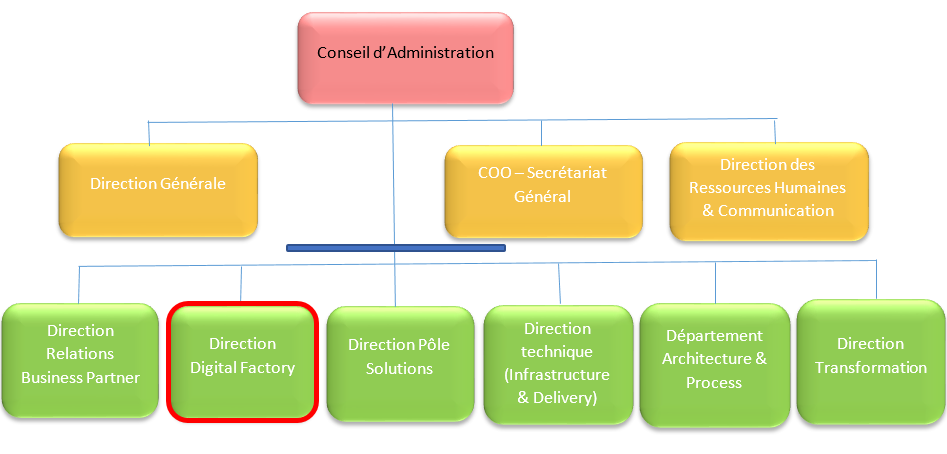
\includegraphics[width=15cm]{images/contexte/ogranigramme2.png}
        \caption{Organigramme de la SG ABS}
\end{figure}
\medskip

\newpage

\subsection{Présentation de la Digital Factory}
\textbf{\large{La raison d'être et les objectifs de la Digital Factory SGABS}}

\medskip
Face aux opportunités stratégiques offertes par le numérique pour le groupe Société Générale, l'entité "Digital Factory" a été créée. Cette entité est chargée de conduire la transformation digitale du groupe et de renforcer la culture numérique.\\

La Digital Factory est un lieu collaboratif et innovant, qui a récemment émergé dans plusieurs entreprises en Europe et aux États-Unis. Il s'agit d'un laboratoire dédié à l'innovation, rassemblant des équipes aux profils pluridisciplinaires engagées dans la transformation globale de l'entreprise.\\

Dans le cadre de cette transformation digitale, la Digital Factory vise à développer des solutions digitales pour les filiales de la région AFS, en travaillant en étroite collaboration avec le Hub Marketing des directions régionales AFS. L'objectif est de répondre rapidement à la concurrence croissante en Afrique. La Digital Factory SGABS devient ainsi un accélérateur de la transformation digitale pour les filiales AFS et a mis en place :

\begin{itemize}
    \item[•] Un Product Management Agile, pour construire de manière itérative et progressive des produits basés sur la valeur.
    \item[•] Une approche centrée sur le client (UX Design), visant à accroître la satisfaction client en termes de qualité et de délai.
    \item[•] L'industrialisation des processus de livraison des mises à jour (CI/CD), afin de réduire le Time To Market.
    \item[•] La mise en place de provisionnement automatique des environnements, permettant une meilleure maîtrise du retour sur investissement (ROI) des infrastructures de nos solutions digitales.
    \item[•] La garantie d'une interopérabilité fonctionnelle et technologique grâce à une plateforme digitale évolutive et innovante.
    \item[•] La création d'usines logicielles pour fiabiliser la conception et la réalisation des solutions digitales.
    \item[•] Toutes ces initiatives contribuent à servir le continent africain depuis l'Afrique, en partageant des sensibilités et des cultures communes.\\
\end{itemize}

\textbf{\large{Types de projets}}
\medskip
\begin{itemize}
    \item[•] Solutions innovantes multicanales (web, mobile, digital corner) au bénéfice des clients ou des collaborateurs.
    \item[•] Projets qui ne nécessitent pas une évolution du CBS (Core Banking System) (hors interfaces - SMG/API).
    \item[•] Développements internes.\\
\end{itemize}

\textbf{\large{Organisation}}

\medskip
La Digital Factory est organisée en quatre équipes pluridisciplinaires, fonctionnant en mode Agile et en interaction avec les fonctions supports centrales (Architecture, GTS, Compliance, Marketing, Architecture, etc.) et les filiales.\\

L'organisation des équipes de la Digital Factory est présentée dans la figure suivante :

\begin{figure}[!h]
    \centering
        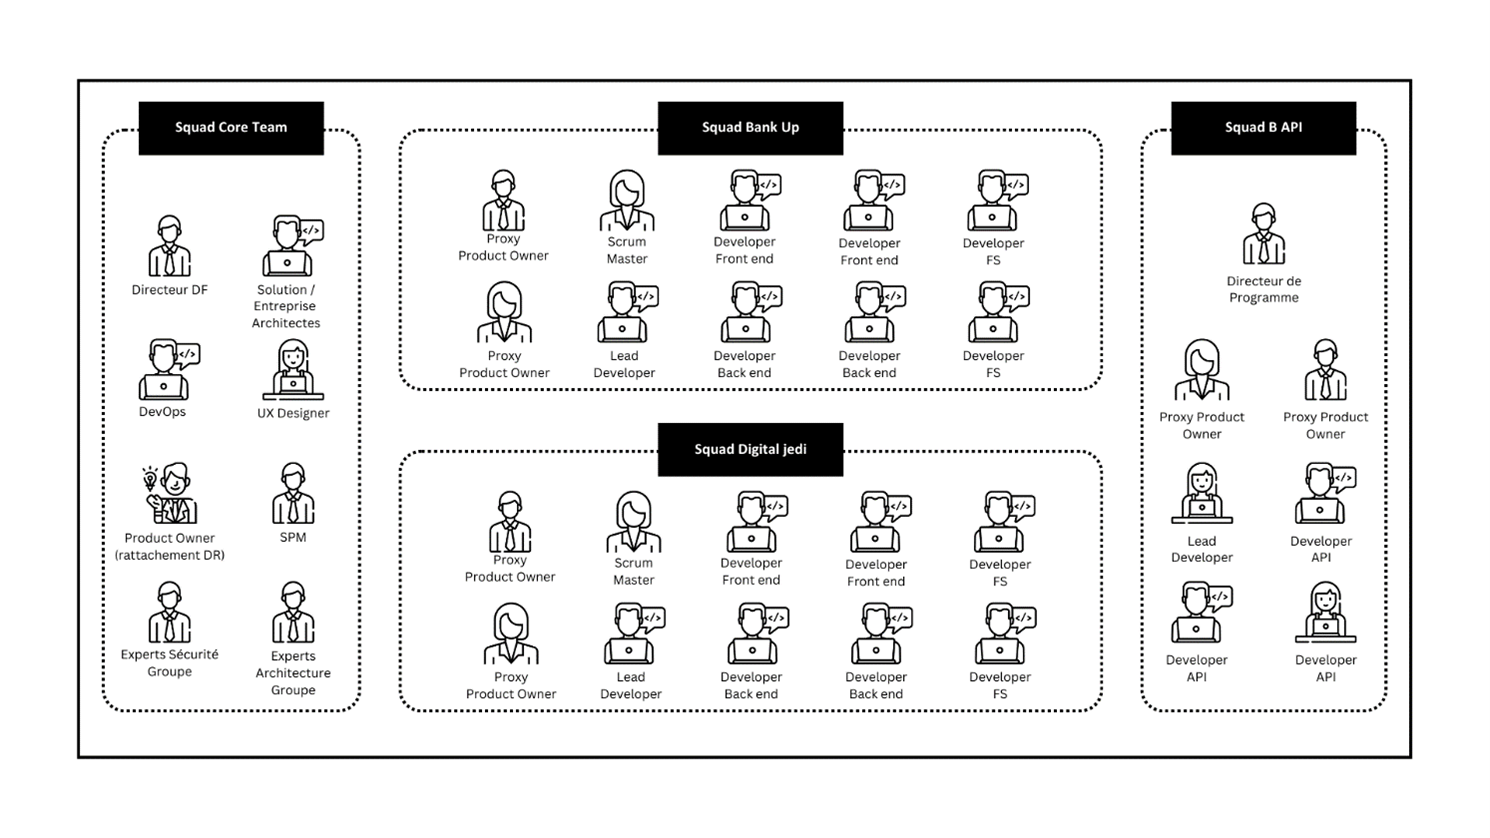
\includegraphics[width=15cm]{images/contexte/Difa.png}
        \caption{Organigramme de la Digital Factory}
\end{figure}

\begin{itemize}
    \item[•] \textbf{Core Team} : Cette équipe est composée d'un Directeur de la Digital Factory, de Solution Architectes, DevOps, UX Designer, Product Owner, SPM, Experts Sécurité Groupe et Experts Architecture Groupe. Cette équipe interagit avec tous les projets des autres équipes de la Digital Factory.
    \item[•] \textbf{Digital JEDI / OPEN R} : Cette équipe s'inscrit dans la stratégie de digitalisation de la banque, visant à rattraper la concurrence et à orienter le flux actuel de clients Retail de l'agence vers la zone digitale. Elle se focalise sur l'industrialisation des deux processus développés au Ghana : "Open App" (application) destinée à l'ouverture de comptes Retail en agences et hors agences (entreprises, universités, etc.) et "Digit" (application bancaire Digital Corner accessible 24/7 sur des zones digitales, dotée des fonctionnalités nécessaires pour couvrir les besoins quotidiens des clients).
    \item[•] \textbf{B-API / UNIBANK} : Cette équipe permet de connecter rapidement les applications (hébergées en interne ou externe) aux CBS des différentes filiales de la zone AFS. Elle assure un accès unifié et sécurisé (authentification de l'utilisateur basée sur des standards, gestion des habilitations et piste d'audit) en faisant abstraction des SMGs sous forme d'APIs (Application Programming Interface). B-API est une composante technique structurante de la plateforme Digital Banking construite avec le projet Bank-UP.
    \item[•] \textbf{Bank-UP} : Cette équipe a pour objectif la mise en place d'une plateforme digitale mutualisée au service des filiales de la Zone AFS. Il s'agit d'une application bancaire en ligne (web et mobile) conforme aux attentes du Groupe en termes de time to market, sécurité, risques opérationnels et solution In-house avec propriété du code source et garantie d'évolutivité de la plateforme.\\
\end{itemize}

\section{Présentation du contexte du projet }
\subsection{Contexte du projet}
La transformation numérique est devenue un enjeu économique et sociétal majeur, remettant en question les modèles économiques, les processus de travail et les relations professionnelles. Dans ce contexte de disruption technologique et de complexité croissante des écosystèmes économiques, la SGABS a pris l'initiative de se transformer pour rester compétitive. Pour cela, elle a établi une vision stratégique claire, basée sur des plans d'action transparents et partagés en interne.\\

La mise en place de la plateforme digitale SG CONNECT fait partie intégrante de cette vision stratégique. Cette plateforme est composée de bibliothèques front-end (web, mobile) contenant les parcours clients, ainsi que d'une couche d'API permettant de masquer la complexité technique vis-à-vis des applications communiquant avec le système d'information de la SGABS. Cette approche d'Open Banking favorise l'ouverture du système d'information de la SGABS et facilite le partage sécurisé des données avec des tiers, dans le respect du consentement des clients.\\

Ce projet s'inscrit dans une démarche plus large de digitalisation de gestion optimale des produits bancaires et de l'expérience client, en leur offrant une expérience bancaire numérique moderne, personnalisée et sécurisée. Il s'appuie sur le moteur Back-End du projet UNIBANK, qui fait partie de la roadmap des projets planifiés par la Digital Factory de la SGABS.

\subsection{Problématique}
Dans un monde de plus en plus numérique et connecté, l'accès facile et pratique aux informations financières est devenu une attente primordiale des clients bancaires. Le projet d'ajout de nouvelles fonctionnalités dans l'application SG CONNECT, développé par l'équipe Bank UP, vise à répondre à cette demande en offrant aux clients de la Société Générale des fonctionnalités avancées liées à leurs cartes monétiques, transactions et produits souscrits.\\

Actuellement, les clients rencontrent plusieurs problématiques lorsqu'ils souhaitent consulter les informations relatives à leurs cartes monétiques. Ils manquent d'une vue d'ensemble claire de leurs cartes et des transactions qui y sont associées. De plus, la connaissance des plafonds nationaux et internationaux associés à chaque carte peut être limitée, ce qui peut entraîner des difficultés lors de voyages ou de transactions spécifiques.\\

De même, l'accès aux détails de leurs produits souscrits représente un défi pour les clients. Ils peuvent se retrouver dans une situation où ils ne sont pas en mesure de visualiser facilement les produits qu'ils ont souscrits, tels que des comptes spécifiques, des prêts ou des services financiers complémentaires. Cela entraîne une confusion et un manque de transparence dans la gestion de leurs finances.\\

Le projet vise donc à résoudre ces problématiques en ajoutant de nouvelles fonctionnalités dans l'application SG CONNECT. Les clients pourront désormais accéder à une vue claire de leurs cartes monétiques, avec la possibilité de consulter les transactions associées à chacune d'entre elles. De plus, ils auront la possibilité de visualiser et de gérer les plafonds nationaux et internationaux de leurs cartes, offrant ainsi un meilleur contrôle de leurs transactions.\\

En ce qui concerne les produits souscrits, les clients pourront consulter facilement les détails et les caractéristiques de leurs comptes, prêts et autres services financiers. Cette fonctionnalité offrira une visibilité accrue sur les engagements financiers des clients, ainsi qu'une meilleure compréhension des conditions et des avantages associés à chaque produit.\\

En résolvant ces problématiques, le projet vise à améliorer l'expérience client en offrant un accès pratique, transparent et autonome aux informations financières. Les clients pourront ainsi gérer leurs finances de manière plus efficace et prendre des décisions éclairées en fonction de leurs besoins et de leurs objectifs.

\subsection{Besoins et objectifs}
Le projet d'ajout de nouvelles fonctionnalités dans l'application SG CONNECT, mené par l'équipe Bank UP, a été initié pour répondre aux besoins et objectifs suivants :

\begin{itemize}
    \item[•] \textbf{Améliorer l'accessibilité aux informations financières} : Les clients de la Société Générale recherchent une plateforme conviviale et pratique pour accéder à leurs données financières. Ils souhaitent consulter facilement les détails de leurs cartes monétiques, les transactions effectuées et les plafonds associés. De plus, ils ont besoin d'un moyen simple et rapide pour visualiser les produits qu'ils ont souscrits, tels que les comptes, les prêts et autres services financiers.
    \item[•] \textbf{Renforcer la transparence et la gestion des finances personnelles} : Les clients souhaitent avoir une vue claire et complète de leurs finances. Ils ont besoin de comprendre les mouvements sur leurs cartes, les transactions effectuées, ainsi que les plafonds de dépenses autorisés. De plus, ils cherchent à avoir une vision globale de leurs produits souscrits, avec une compréhension claire des conditions, des avantages et des échéances associés.
    \item[•] \textbf{Offrir une meilleure autonomie et flexibilité} : Les clients souhaitent être en mesure de gérer leurs finances de manière autonome, sans dépendre systématiquement de l'assistance d'un conseiller en agence. Ils veulent pouvoir ajuster les plafonds de leurs cartes selon leurs besoins, consulter rapidement leurs transactions passées et actuelles, et obtenir des informations précises sur leurs produits financiers, sans contraintes de temps ni de lieu.
    \item[•] \textbf{Renforcer la confiance et la fidélité des clients} : En offrant des fonctionnalités avancées et une expérience utilisateur améliorée, le projet vise à renforcer la confiance des clients envers la Société Générale. Les clients bénéficieront d'un accès sécurisé à leurs données financières, d'une transparence accrue dans la gestion de leurs comptes et de la possibilité de prendre des décisions éclairées en matière de finances personnelles. Cela contribuera à renforcer la satisfaction et la fidélité des clients envers la banque.
\end{itemize}
En répondant à ces besoins et objectifs, le projet d'ajout de nouvelles fonctionnalités dans l'application SG CONNECT vise à offrir une expérience client optimisée, en mettant à disposition des outils et des informations essentiels pour la gestion de leurs finances personnelles. En mettant l'accent sur l'accessibilité, la transparence et l'autonomie, l'équipe Bank UP aspire à fournir une solution complète qui répond aux attentes des clients et les accompagne dans leur parcours financier.

\section{Conduite du projet}
\subsection{Méthodologie de travail : SCRUM}
La conduite de ce projet s'appuie sur la méthodologie SCRUM, adoptée par l'équipe de la Digital Factory pour garantir des résultats rapides et un time to market réduit. SCRUM est une approche agile qui permet une meilleure organisation des différentes phases du projet, en accordant une importance primordiale à l'implication et à la participation active du client tout au long du processus de développement. En suivant SCRUM, nous visons à améliorer la productivité de notre équipe, à respecter les délais fixés et à assurer le bon déroulement général du projet.

\begin{figure}[!h]
    \centering %
        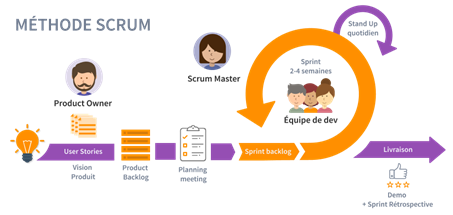
\includegraphics[width=14cm]{images/conduite/SCRUM.png}
    \caption{Méthode SCRUM}
\end{figure}

\textbf{\large{Les avantages de la méthode SCRUM}}
\medskip
\begin{itemize}
    \item[•] \textbf{Personnel engagé :} SCRUM favorise l'engagement du personnel en les impliquant activement dans la définition des activités et des horaires, ce qui conduit à une plus grande motivation et implication.
    \item[•] \textbf{Meilleure vue d’ensemble du projet :} SCRUM permet à tous les membres de l'équipe d'avoir une compréhension homogène des objectifs et des tâches à accomplir, offrant ainsi une meilleure vue d'ensemble du projet.
    \item[•] \textbf{Mise à jour des priorités :} Avec SCRUM, le client bénéficie d'une flexibilité au niveau de la définition et de l'évolution des priorités et des séquences d'activités, permettant une adaptation aux besoins changeants.
    \item[•] \textbf{Qualité du produit mise en avant :} SCRUM se concentre davantage sur la fourniture d'un service de valeur au client plutôt que sur une date limite stricte, mettant ainsi en avant la qualité du produit.
    \item[•] \textbf{Communication renforcée :} SCRUM favorise une communication régulière et transparente au sein de l'équipe, permettant une collaboration efficace et une résolution rapide des problèmes.
    \item[•] \textbf{Réduction des risques :} En utilisant des itérations courtes et des revues régulières, SCRUM permet de détecter et de résoudre les problèmes plus rapidement, réduisant ainsi les risques liés au projet.\\
\end{itemize}


\textbf{\large{Répartition des rôles dans SCRUM}}
\medskip
\begin{itemize}
    \item[•] \textbf{Le Scrum Master :} Il est responsable de la compréhension, de l'adhésion et de la mise en œuvre de la méthode SCRUM. Le Scrum Master facilite la communication au sein de l'équipe et cherche à maximiser sa productivité. Il veille également au respect des principes et des valeurs de SCRUM.
    \item[•] \textbf{Le Product Owner :} Il porte la vision du produit à réaliser et travaille en interaction avec l'équipe de développement. Le Product Owner établit les priorités des fonctionnalités à développer ou à corriger et valide les fonctionnalités terminées. Il est responsable de la gestion du product backlog et s'assure que les besoins du client sont correctement pris en compte.
    \item[•] \textbf{L'équipe de développement :} Elle est chargée de transformer les besoins définis par le Product Owner en fonctionnalités utilisables. Les décisions au sein de l'équipe de développement sont prises collectivement, sans notion de hiérarchie.\\
\end{itemize}


\textbf{\large{Les différents événements de la SCRUM}}
\medskip
\begin{itemize}
    \item[•] \textbf{Le sprint :} Il s'agit d'une itération de quelques semaines pendant laquelle une version terminée et utilisable du produit est réalisée. Un nouveau sprint commence immédiatement après la fin du précédent. Chaque sprint a un objectif clair et une liste de fonctionnalités à réaliser.
    \item[•] \textbf{La planification d'un sprint :} C'est une réunion qui précède le début d'un sprint et qui vise à définir les tâches à accomplir pendant cette période. L'équipe de développement et le Product Owner collaborent pour déterminer les objectifs et les priorités du sprint.
    \item[•] \textbf{La revue de sprint :} À la fin de chaque sprint, une réunion de revue est organisée pour présenter les fonctionnalités réalisées à l'équipe de développement et aux parties prenantes. C'est l'occasion de valider ce qui a été accompli et de recueillir des feedbacks.
    \item[•] \textbf{La rétrospective de sprint :} Elle se tient après la revue de sprint et permet à l'équipe de passer en revue le sprint écoulé afin d'identifier les aspects positifs, les problèmes rencontrés et les opportunités d'amélioration. Cela permet d'ajuster les pratiques et d'optimiser la performance pour les sprints suivants.
    \item[•] \textbf{Le daily scrum :} C'est une réunion quotidienne de courte durée au cours de laquelle l'équipe de développement fait le point sur sa progression. Les membres de l'équipe répondent à trois questions clés : qu'ont-ils réalisé la veille, qu'accompliront-ils aujourd'hui et quels sont les obstacles éventuels.\\
\end{itemize}

\textbf{\large{Les artefacts de SCRUM}}
\medskip
\begin{itemize}
    \item[•] \textbf{Le product backlog :} Il s'agit d'une liste hiérarchisée des exigences initiales du client concernant le produit à réaliser. Ce document évolue tout au long du projet en fonction des besoins du client, et le Product Owner en est responsable.
    \item[•] \textbf{Le sprint backlog :} Il représente le plan détaillé de la réalisation des objectifs d'un sprint, regroupant l'ensemble des user stories que l'équipe s'est engagée à accomplir. Il est défini lors de la réunion de planification du sprint et est régulièrement mis à jour pour suivre la progression.
    \item[•] \textbf{L'incrément :} Il correspond à la somme des éléments terminés du product backlog au cours d'un sprint, ainsi que des incréments des sprints précédents. À la fin d'un sprint, l'incrément doit être "Done", c'est-à-dire utilisable et conforme à la définition de "Done" définie par l'équipe SCRUM. Le Product Owner décide de sa libération ou non.
\end{itemize}

\subsection{Cycle de vie du projet}

\par Afin d’assurer le bon déroulement du projet, nous avons opté pour le cycle de vie suivant :
\begin{itemize}
    \item[$\bullet$] \textbf{Etude de cadrage:} cette étape consiste à bien définir le périmètre fonctionnel du projet. Elle permet de comprendre et analyser la structure de l’existant pour bien cadrer les besoins du client afin d’aboutir à un résultat qui s’aligne parfaitement avec ses attentes.
    \item[$\bullet$] \textbf{Spécifications et analyse des besoins:} cette phase permet de spécifier les besoins
définis dans la précédente phase du projet. Elle est d’une grande signification, 
    \item[$\bullet$] \textbf{Développement:} C'est la partie où l'on développe les fonctionnalités et les besoins exprimés lors de la phase précédente. L'objectif est de produire des services conformes aux spécifications exprimées par le métier tout en respectant un ensemble de règles de gestion technique et de bonnes pratiques.
    \item[$\bullet$] \textbf{Tests et validation:} Ils sont réalisés à la fin de chaque Sprint pour valider le travail réalisé avec le client.
    \item[$\bullet$] \textbf{Déploiement:} C'est la partie où les services développés et testés sont déployés dans un environnement accessible au client pour qu'il puisse les utiliser.
    \item[$\bullet$] \textbf{Monitoring:} À ce niveau, nous gardons un œil sur l'application en cours d'exécution et sommes prêts pour résoudre tout problème lorsqu'il se produit. 
\end{itemize}


\subsection{Planification du projet}
Pour gérer le projet et aboutir aux objectifs fixés ci-dessus, nous avons suivi les étapes représentées dans le diagramme de GANTT suivant :

\begin{figure}[!h]
    \centering %
        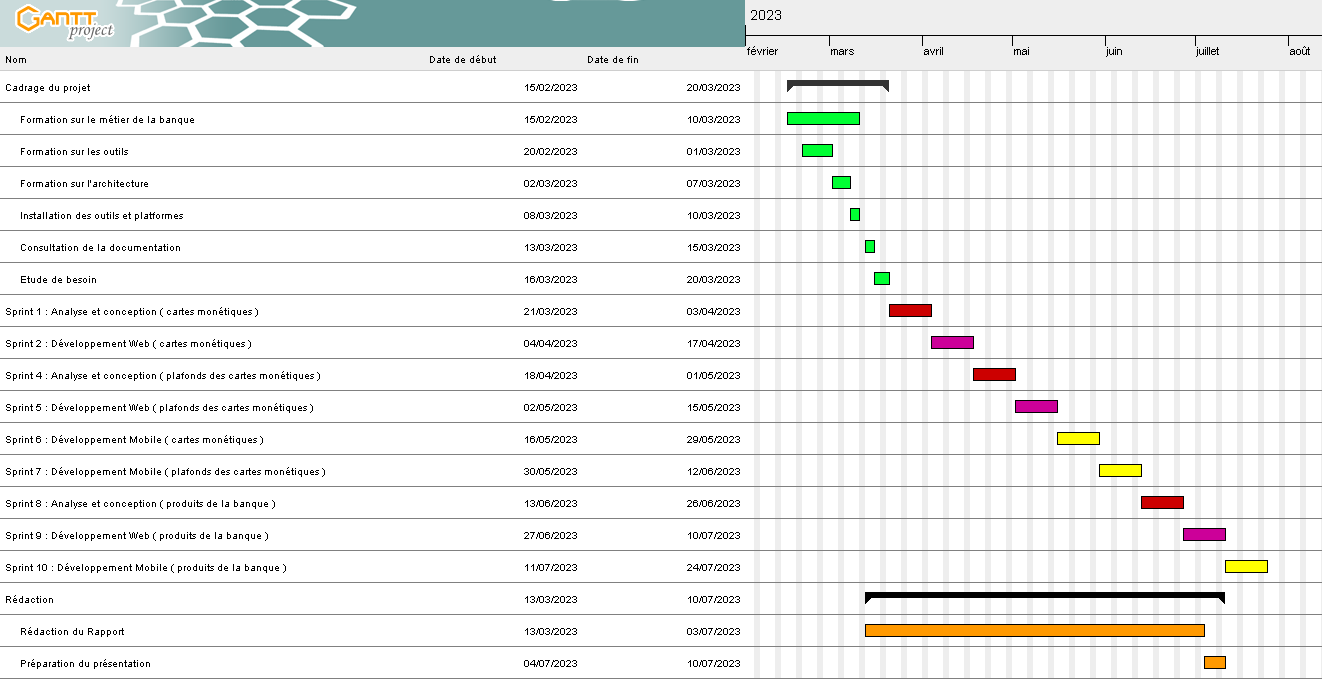
\includegraphics[width=16cm]{images/conduite/gantt.png}
    \caption{Diagramme de Gantt}
\end{figure}

\newpage

La phase de planification du projet a débuté par une étape de cadrage, au cours de laquelle nous avons bénéficié de formations approfondies afin de comprendre le domaine bancaire et de nous familiariser avec les exigences spécifiques du projet. Cette phase nous a permis de mener une étude approfondie des besoins et de spécifier les fonctionnalités à mettre en œuvre.\\

Pour mettre en pratique la méthodologie SCRUM, nous avons créé un backlog qui regroupe toutes les fonctionnalités requises sous forme de user stories. Lors de la réunion de planification du sprint, appelée "sprint planning", nous avons sélectionné les user stories sur lesquelles nous allons travailler pour chaque sprint. Ensuite, nous avons procédé à l'analyse et à la conception de chaque fonctionnalité, avant de passer à sa mise en œuvre.\\

Le développement de chaque fonctionnalité s'est déroulé au sein de sprints définis, où elle a été développée, testée, corrigée et déployée. À la fin de chaque sprint, nous avons obtenu une version fonctionnelle du produit, prête à être évaluée et validée par l'équipe de développement et les parties prenantes.\\

Cette approche itérative nous a permis de travailler de manière efficace et d'assurer une progression continue du projet, tout en offrant une flexibilité pour s'adapter aux éventuels changements de priorités ou de besoins.


\subsection{Outils de gestion de projet}

Pour mener à bien le projet, l'utilisation d'outils de gestion est essentielle afin de faciliter le travail d'équipe et de garantir le respect de la méthodologie Scrum. Trois outils ont été employés dans ce contexte : Jira, Microsoft Teams et Confluence.

\begin{itemize}
\item[$\bullet$] \textbf{Jira}
\end{itemize}
Jira a été utilisé comme outil de gestion de projet en ligne par la Société Générale African Business Services. Il s'agit d'une plateforme polyvalente qui facilite la gestion de projet en permettant le suivi des tâches, l'identification des obstacles et le partage d'informations au sein de l'équipe. Jira est basé sur l'organisation des projets en tickets, chacun représentant une tâche spécifique. Il offre également la possibilité de suivre l'état des tickets et de définir un flux de travail adapté aux méthodes de travail.\\
Jira génère des graphiques et des visualisations qui permettent de visualiser rapidement l'état des différentes missions et d'identifier les problèmes à résoudre en priorité.\\
Dans notre projet, Jira a été utilisé pour publier les User Stories, organiser les sprints et le backlog, suivre les tâches et sous-tâches, ainsi que pour estimer l'effort de l'équipe.
\begin{figure}[!h]
    \centering %
        
\includegraphics[height=3cm]{images/logos/jira.png}
    \caption{Logo de Jira}
\end{figure}

\begin{itemize}
    \item[$\bullet$] \textbf{Microsoft Teams}
    \end{itemize}
    Microsoft Teams a été utilisé pour organiser les réunions entre les membres de l'équipe. Cet outil a permis aux membres de l'équipe de communiquer, de planifier les tâches, de partager des astuces utiles, de discuter des progrès réalisés, des tâches à accomplir et des difficultés rencontrées. Des sessions de formation ont également été programmées pour renforcer la compréhension des fondements du métier bancaire dans notre domaine. Microsoft Teams a également été utilisé pour planifier les différentes cérémonies Scrum.
    \begin{figure}[!h]
        \centering %
            
\includegraphics[height=3cm]{images/logos/microsoftTeams.png}
        \caption{Logo de Microsoft Teams}
    \end{figure}

    \begin{itemize}
        \item[$\bullet$] \textbf{Confluence}
        \end{itemize}
        Confluence est une solution de travail collaboratif qui permet de créer et de stocker des fichiers sur une plateforme unique. Il offre la possibilité de créer des pages à partir de zéro ou d'utiliser des modèles personnalisables parmi une large sélection. Les pages créées peuvent être enrichies en commentaires, images, vidéos ou GIF, et peuvent être liées dans un espace dédié, permettant aux membres de l'équipe de partager leurs impressions, de demander de l'aide et de faciliter la prise de décision.
        \begin{figure}[!h]
            \centering %
                
\includegraphics[height=3cm]{images/logos/Confluence.png}
            \caption{Logo de Confluence}
        \end{figure}

Ces trois outils ont joué un rôle essentiel dans la gestion du projet en favorisant la collaboration, l'organisation et le partage d'informations au sein de l'équipe de développement.

\newpage

\section{Conclusion}
En conclusion, nous avons présenté le cadre générale du projet, l'organisme d'accueil, son historique, ses objectifs et ses activités, puis nous avons passé à la méthodologie adoptée, le cycle de vie du projet et la planification à l'aide du diagramme de Gantt. Nous avons également examiné les outils de gestion du projet utilisés pour faciliter la coordination et le suivi de l'équipe. Ces éléments sont essentiels pour assurer une gestion efficace du projet, respecter les délais et atteindre les objectifs fixés.\\
Dans le chapitre suivant, nous aborderons l'analyse des besoins, la modélisation et la conception du projet.
% % \addcontentsline{toc}{chapter}{Chapitre 2} 
\chapter{Conduite du projet}

Ce chapitre est consacré à la conduite du projet. Il présente la méthodologie adoptée pour la conduite du projet ainsi que son plan et les outils utilisés pour faire la gestion de ce projet.

\clearpage
\label{sec:organisme}

\section{Introduction}
Dans le cadre de la conduite du projet d'ajout de nouvelles fonctionnalités dans l'application SG CONNECT, notre équipe, Bank UP, suit la méthodologie SCRUM. Notre priorité absolue est de satisfaire le client en fournissant rapidement des fonctionnalités à valeur ajoutée, en tirant parti du changement comme une opportunité. Dans ce chapitre, nous détaillerons les composants et les démarches de SCRUM que nous utilisons pour mener à bien ce projet, de la planification à la livraison finale. Notre approche SCRUM nous permet d'offrir des résultats de haute qualité dans des délais raisonnables, en favorisant la flexibilité et l'adaptation continue aux besoins changeants du projet.

\section{Méthodologie de travail : SCRUM}
La conduite de ce projet s'appuie sur la méthodologie SCRUM, adoptée par l'équipe de la Digital Factory pour garantir des résultats rapides et un time to market réduit. SCRUM est une approche agile qui permet une meilleure organisation des différentes phases du projet, en accordant une importance primordiale à l'implication et à la participation active du client tout au long du processus de développement. En suivant SCRUM, nous visons à améliorer la productivité de notre équipe, à respecter les délais fixés et à assurer le bon déroulement général du projet.

\begin{figure}[!h]
    \centering %
        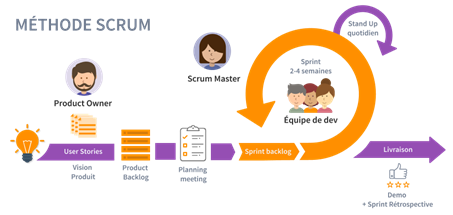
\includegraphics[width=14cm]{images/conduite/SCRUM.png}
    \caption{Méthode SCRUM}
\end{figure}

\textbf{\large{Les avantages de la méthode SCRUM}}
\medskip
\begin{itemize}
    \item[•] \textbf{Personnel engagé :} SCRUM favorise l'engagement du personnel en les impliquant activement dans la définition des activités et des horaires, ce qui conduit à une plus grande motivation et implication.
    \item[•] \textbf{Meilleure vue d’ensemble du projet :} SCRUM permet à tous les membres de l'équipe d'avoir une compréhension homogène des objectifs et des tâches à accomplir, offrant ainsi une meilleure vue d'ensemble du projet.
    \item[•] \textbf{Mise à jour des priorités :} Avec SCRUM, le client bénéficie d'une flexibilité au niveau de la définition et de l'évolution des priorités et des séquences d'activités, permettant une adaptation aux besoins changeants.
    \item[•] \textbf{Qualité du produit mise en avant :} SCRUM se concentre davantage sur la fourniture d'un service de valeur au client plutôt que sur une date limite stricte, mettant ainsi en avant la qualité du produit.
    \item[•] \textbf{Communication renforcée :} SCRUM favorise une communication régulière et transparente au sein de l'équipe, permettant une collaboration efficace et une résolution rapide des problèmes.
    \item[•] \textbf{Réduction des risques :} En utilisant des itérations courtes et des revues régulières, SCRUM permet de détecter et de résoudre les problèmes plus rapidement, réduisant ainsi les risques liés au projet.\\
\end{itemize}


\textbf{\large{Répartition des rôles dans SCRUM}}
\medskip
\begin{itemize}
    \item[•] \textbf{Le Scrum Master :} Il est responsable de la compréhension, de l'adhésion et de la mise en œuvre de la méthode SCRUM. Le Scrum Master facilite la communication au sein de l'équipe et cherche à maximiser sa productivité. Il veille également au respect des principes et des valeurs de SCRUM.
    \item[•] \textbf{Le Product Owner :} Il porte la vision du produit à réaliser et travaille en interaction avec l'équipe de développement. Le Product Owner établit les priorités des fonctionnalités à développer ou à corriger et valide les fonctionnalités terminées. Il est responsable de la gestion du product backlog et s'assure que les besoins du client sont correctement pris en compte.
    \item[•] \textbf{L'équipe de développement :} Elle est chargée de transformer les besoins définis par le Product Owner en fonctionnalités utilisables. Les décisions au sein de l'équipe de développement sont prises collectivement, sans notion de hiérarchie.\\
\end{itemize}


\textbf{\large{Les différents événements de la SCRUM}}
\medskip
\begin{itemize}
    \item[•] \textbf{Le sprint :} Il s'agit d'une itération de quelques semaines pendant laquelle une version terminée et utilisable du produit est réalisée. Un nouveau sprint commence immédiatement après la fin du précédent. Chaque sprint a un objectif clair et une liste de fonctionnalités à réaliser.
    \item[•] \textbf{La planification d'un sprint :} C'est une réunion qui précède le début d'un sprint et qui vise à définir les tâches à accomplir pendant cette période. L'équipe de développement et le Product Owner collaborent pour déterminer les objectifs et les priorités du sprint.
    \item[•] \textbf{La revue de sprint :} À la fin de chaque sprint, une réunion de revue est organisée pour présenter les fonctionnalités réalisées à l'équipe de développement et aux parties prenantes. C'est l'occasion de valider ce qui a été accompli et de recueillir des feedbacks.
    \item[•] \textbf{La rétrospective de sprint :} Elle se tient après la revue de sprint et permet à l'équipe de passer en revue le sprint écoulé afin d'identifier les aspects positifs, les problèmes rencontrés et les opportunités d'amélioration. Cela permet d'ajuster les pratiques et d'optimiser la performance pour les sprints suivants.
    \item[•] \textbf{Le daily scrum :} C'est une réunion quotidienne de courte durée au cours de laquelle l'équipe de développement fait le point sur sa progression. Les membres de l'équipe répondent à trois questions clés : qu'ont-ils réalisé la veille, qu'accompliront-ils aujourd'hui et quels sont les obstacles éventuels.\\
\end{itemize}

\textbf{\large{Les artefacts de SCRUM}}
\medskip
\begin{itemize}
    \item[•] \textbf{Le product backlog :} Il s'agit d'une liste hiérarchisée des exigences initiales du client concernant le produit à réaliser. Ce document évolue tout au long du projet en fonction des besoins du client, et le Product Owner en est responsable.
    \item[•] \textbf{Le sprint backlog :} Il représente le plan détaillé de la réalisation des objectifs d'un sprint, regroupant l'ensemble des user stories que l'équipe s'est engagée à accomplir. Il est défini lors de la réunion de planification du sprint et est régulièrement mis à jour pour suivre la progression.
    \item[•] \textbf{L'incrément :} Il correspond à la somme des éléments terminés du product backlog au cours d'un sprint, ainsi que des incréments des sprints précédents. À la fin d'un sprint, l'incrément doit être "Done", c'est-à-dire utilisable et conforme à la définition de "Done" définie par l'équipe SCRUM. Le Product Owner décide de sa libération ou non.
\end{itemize}


\section{Cycle de vie du projet}

\par Afin d’assurer le bon déroulement du projet, nous avons opté pour le cycle de vie suivant :
\begin{itemize}
    \item[$\bullet$] \textbf{Etude de cadrage:} cette étape consiste à bien définir le périmètre fonctionnel du projet. Elle permet de comprendre et analyser la structure de l’existant pour bien cadrer les besoins du client afin d’aboutir à un résultat qui s’aligne parfaitement avec ses attentes.
    \item[$\bullet$] \textbf{Spécifications et analyse des besoins:} cette phase permet de spécifier les besoins
définis dans la précédente phase du projet. Elle est d’une grande signification, 
    \item[$\bullet$] \textbf{Développement:} C'est la partie où l'on développe les fonctionnalités et les besoins exprimés lors de la phase précédente. L'objectif est de produire des services conformes aux spécifications exprimées par le métier tout en respectant un ensemble de règles de gestion technique et de bonnes pratiques.
    \item[$\bullet$] \textbf{Tests et validation:} Ils sont réalisés à la fin de chaque Sprint pour valider le travail réalisé avec le client.
    \item[$\bullet$] \textbf{Déploiement:} C'est la partie où les services développés et testés sont déployés dans un environnement accessible au client pour qu'il puisse les utiliser.
    \item[$\bullet$] \textbf{Monitoring:} À ce niveau, nous gardons un œil sur l'application en cours d'exécution et sommes prêts pour résoudre tout problème lorsqu'il se produit. 
\end{itemize}


\section{Planification du projet}
Pour gérer le projet et aboutir aux objectifs fixés ci-dessus, nous avons suivi les étapes représentées dans le diagramme de GANTT suivant :

\begin{figure}[!h]
    \centering %
        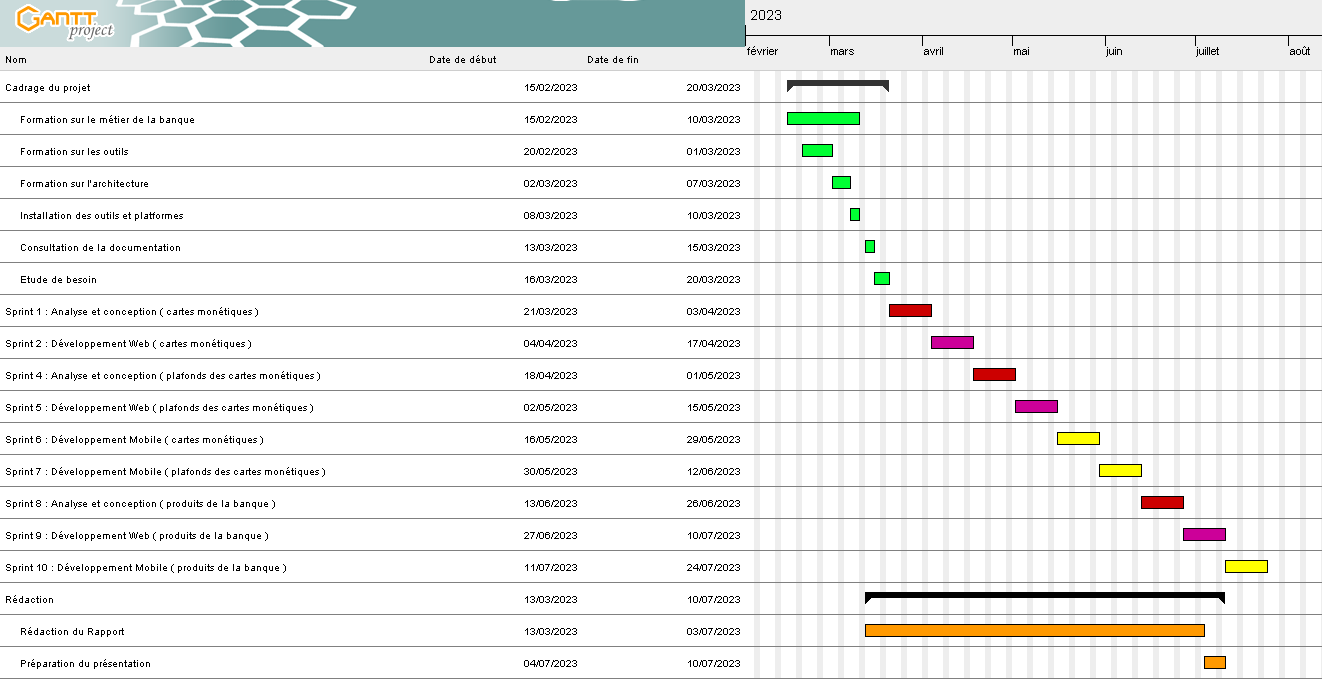
\includegraphics[width=16cm]{images/conduite/gantt.png}
    \caption{Diagramme de Gantt}
\end{figure}

\newpage

La phase de planification du projet a débuté par une étape de cadrage, au cours de laquelle nous avons bénéficié de formations approfondies afin de comprendre le domaine bancaire et de nous familiariser avec les exigences spécifiques du projet. Cette phase nous a permis de mener une étude approfondie des besoins et de spécifier les fonctionnalités à mettre en œuvre.\\

Pour mettre en pratique la méthodologie SCRUM, nous avons créé un backlog qui regroupe toutes les fonctionnalités requises sous forme de user stories. Lors de la réunion de planification du sprint, appelée "sprint planning", nous avons sélectionné les user stories sur lesquelles nous allons travailler pour chaque sprint. Ensuite, nous avons procédé à l'analyse et à la conception de chaque fonctionnalité, avant de passer à sa mise en œuvre.\\

Le développement de chaque fonctionnalité s'est déroulé au sein de sprints définis, où elle a été développée, testée, corrigée et déployée. À la fin de chaque sprint, nous avons obtenu une version fonctionnelle du produit, prête à être évaluée et validée par l'équipe de développement et les parties prenantes.\\

Cette approche itérative nous a permis de travailler de manière efficace et d'assurer une progression continue du projet, tout en offrant une flexibilité pour s'adapter aux éventuels changements de priorités ou de besoins.


\section{Outils de gestion de projet}

Pour mener à bien le projet, l'utilisation d'outils de gestion est essentielle afin de faciliter le travail d'équipe et de garantir le respect de la méthodologie Scrum. Trois outils ont été employés dans ce contexte : Jira, Microsoft Teams et Confluence.

\begin{itemize}
\item[$\bullet$] \textbf{Jira}
\end{itemize}
Jira a été utilisé comme outil de gestion de projet en ligne par la Société Générale African Business Services. Il s'agit d'une plateforme polyvalente qui facilite la gestion de projet en permettant le suivi des tâches, l'identification des obstacles et le partage d'informations au sein de l'équipe. Jira est basé sur l'organisation des projets en tickets, chacun représentant une tâche spécifique. Il offre également la possibilité de suivre l'état des tickets et de définir un flux de travail adapté aux méthodes de travail.\\
Jira génère des graphiques et des visualisations qui permettent de visualiser rapidement l'état des différentes missions et d'identifier les problèmes à résoudre en priorité.\\
Dans notre projet, Jira a été utilisé pour publier les User Stories, organiser les sprints et le backlog, suivre les tâches et sous-tâches, ainsi que pour estimer l'effort de l'équipe.
\begin{figure}[!h]
    \centering %
        
\includegraphics[height=3cm]{images/logos/jira.png}
    \caption{Logo de Jira}
\end{figure}

\begin{itemize}
    \item[$\bullet$] \textbf{Microsoft Teams}
    \end{itemize}
    Microsoft Teams a été utilisé pour organiser les réunions entre les membres de l'équipe. Cet outil a permis aux membres de l'équipe de communiquer, de planifier les tâches, de partager des astuces utiles, de discuter des progrès réalisés, des tâches à accomplir et des difficultés rencontrées. Des sessions de formation ont également été programmées pour renforcer la compréhension des fondements du métier bancaire dans notre domaine. Microsoft Teams a également été utilisé pour planifier les différentes cérémonies Scrum.
    \begin{figure}[!h]
        \centering %
            
\includegraphics[height=3cm]{images/logos/microsoftTeams.png}
        \caption{Logo de Microsoft Teams}
    \end{figure}

    \begin{itemize}
        \item[$\bullet$] \textbf{Confluence}
        \end{itemize}
        Confluence est une solution de travail collaboratif qui permet de créer et de stocker des fichiers sur une plateforme unique. Il offre la possibilité de créer des pages à partir de zéro ou d'utiliser des modèles personnalisables parmi une large sélection. Les pages créées peuvent être enrichies en commentaires, images, vidéos ou GIF, et peuvent être liées dans un espace dédié, permettant aux membres de l'équipe de partager leurs impressions, de demander de l'aide et de faciliter la prise de décision.
        \begin{figure}[!h]
            \centering %
                
\includegraphics[height=3cm]{images/logos/Confluence.png}
            \caption{Logo de Confluence}
        \end{figure}

Ces trois outils ont joué un rôle essentiel dans la gestion du projet en favorisant la collaboration, l'organisation et le partage d'informations au sein de l'équipe de développement.

\newpage

\section{Conclusion}
En conclusion de ce chapitre sur la conduite de projet, nous avons présenté la méthodologie adoptée, le cycle de vie du projet et la planification à l'aide du diagramme de Gantt. Nous avons également examiné les outils de gestion du projet utilisés pour faciliter la coordination et le suivi de l'équipe. Ces éléments sont essentiels pour assurer une gestion efficace du projet, respecter les délais et atteindre les objectifs fixés.\\
Dans le chapitre suivant, nous aborderons l'analyse des besoins, la modélisation et la conception du projet.
\chapter{Étude détaillée du projet}
\par Ce chapitre est consacré à la description de l'aspect fonctionnel du cycle de développement à travers l'analyse de l'existant, le diagramme des cas d'utilisation et le détail des objectifs techniques fixés pour le projet.


\clearpage
\section{Introduction}
Après avoir défini les objectifs du projet dans le chapitre précédent, nous allons maintenant nous concentrer sur la spécification précise des besoins fonctionnels et non fonctionnels. Cette étape est essentielle pour s'assurer que le système répondra aux attentes des utilisateurs et aux exigences de la Digital Factory. Nous procéderons à une analyse approfondie des fonctionnalités requises, en identifiant les interactions entre les acteurs et le système. \\
Nous examinerons également les contraintes et les exigences non fonctionnelles auxquelles le système doit se conformer. Cette étude détaillée servira de base solide pour la conception de l'architecture du système, qui sera présentée dans les chapitres ultérieurs. Grâce à cette analyse approfondie, nous serons en mesure de proposer une solution optimale qui répondra aux besoins identifiés et garantira la satisfaction des utilisateurs.

\section{Analyse de l'existant}
\subsection{Étude de l'existant}
Dans le cadre de sa stratégie de digitalisation, l'équipe de développement de la Digital Factory au sein de la Société Générale ABS a mis en place une solution web et mobile appelée SG CONNECT. Cette application a été développée dans le but de simplifier, accélérer et sécuriser la gestion des comptes clients en offrant une gamme variée de services bancaires à distance, accessibles 24 heures sur 24 et 7 jours sur 7. Cette solution unique a été déployée pour desservir les 14 filiales de la zone AFMO (Afrique Méditerranée et Outre-mer).\\

SG CONNECT a été conçue pour remplacer les applications existantes telles que Cadinet et Mobilize, ou pour répondre directement aux besoins croissants en matière de services bancaires à distance. Actuellement, l'application est disponible pour les filiales suivantes : Burkina Faso, Madagascar, Mauritanie, Congo, Tchad, Bénin, Côte d'Ivoire, Guinée, Cameroun, Sénégal et Ghana.\\

Dans sa version R2+ actuelle, l'application SG CONNECT propose plusieurs fonctionnalités, dont :

\begin{itemize}
    \item[•] Téléchargement du RIB et des relevés de compte
    \item[•] Localisation des agences et des distributeurs automatiques de billets à proximité
   \item[•] Mode démo
   \item[•] Autres options : CGU \& FAQ et À propos
   \item[•] Consultation des comptes
   \item[•] Gestion des mots de passe : récupération d'un mot de passe oublié et changement de mot de passe
   \item[•] Consultation du taux de change
   \item[•] Graphiques représentant les données financières
   \item[•] Consultation des crédits et placements
   \item[•] Virements compte à compte et virements vers bénéficiaires SG et Confrères
   \item[•] Gestion des bénéficiaires
   \item[•] Recherche dans l'historique des opérations
   \item[•] Historique des virements
   \item[•] Commande de chéquier
  \item[•]  Simulateur de crédit
   \item[•] Souscription à distance
   \item[•] Paramétrage de la langue
   \item[•] Virement Wallet
   \item[•] Gestion des Alias et jauge de solde
   \item[•] Gestion des bénéficiaires Wallet
   \item[•] Gestion des impayés de crédits
   \item[•] Édition du reçu de virement
   \item[•] Affichage des libellés structurés
   \item[•] Contactez-nous
   \item[•] Gestion des alertes
   \item[•] Virement intrarégional
   \item[•] Virement interopérable
   \item[•] Authentification par biométrie et empreinte digitale
   \item[•] Notifications PUSH\\
\end{itemize}

Cependant, il est important de souligner que l'application SG CONNECT repose sur une infrastructure backend solide et sécurisée. Dans ce contexte, la Digital Factory a créé la plateforme digitale UNIBANK pour répondre aux exigences de l'Open Banking et garantir la sécurité et le consentement des clients dans le partage de leurs données financières. UNIBANK est une plateforme d'Open Banking qui ouvre le système d'information de la Société Générale et facilite l'échange sécurisé de données avec des tiers.\\

UNIBANK joue un rôle essentiel en assurant la connectivité et l'interopérabilité entre les applications consommatrices, telles que SG CONNECT, et les APIs développées, en masquant la complexité technique et en garantissant le respect des réglementations sécuritaires. La plateforme UNIBANK est construite sur une technologie open-source appelée WSo2 et comprend plusieurs projets (squads) travaillant sur les différentes couches et briques de son architecture pour assurer la disponibilité et la sécurité des APIs consommées.\\

Ainsi, SG CONNECT constitue l'interface conviviale et intuitive pour les clients, leur offrant un accès facile à une large gamme de services bancaires. En arrière-plan, UNIBANK fournit les fonctionnalités backend et la connectivité nécessaire pour garantir une expérience utilisateur optimale et sécurisée.

\subsection{Limitations de l'existant}
L'application SG CONNECT, bien qu'elle propose déjà un ensemble de fonctionnalités bancaires à distance, présente certaines limitations qui restreignent l'expérience utilisateur et les services offerts. Parmi les principales limitations identifiées, on peut citer l'absence d'affichage des cartes monétiques associées aux comptes des clients, ce qui limite la visibilité et le suivi des transactions liées à ces cartes. De plus, les informations sur les plafonds nationaux et internationaux de chaque carte ne sont pas disponibles, rendant difficile pour les clients de gérer et contrôler leurs dépenses selon leurs besoins spécifiques. De plus, l'application ne fournit pas de visibilité claire sur les produits souscrits par le client pour chaque compte bancaire, ce qui limite la compréhension globale de la situation financière.\\

Ces limitations ont un impact sur l'expérience utilisateur et empêchent les clients d'accéder à des informations cruciales pour gérer efficacement leurs comptes et effectuer des transactions en toute confiance. 

\section{Analyse et identification des besoins}
\subsection{Besoins fonctionnels}
Afin d'atteindre les objectifs souhaités, il est crucial d'identifier avec précision les besoins fonctionnels et non fonctionnels du projet. Les différentes réunions de Backlog Grooming ont permis de spécifier en détail les exigences fonctionnelles que la solution doit satisfaire. L'ensemble de la solution doit répondre aux spécifications fonctionnelles suivantes :

\begin{itemize}
    \item[•] \textbf{Affichage des cartes monétiques :} L'application doit permettre aux utilisateurs de visualiser toutes leurs cartes monétiques associées à leurs comptes bancaires, avec des informations détaillées telles que le type de carte, le numéro de carte et la date d'expiration.
    \item[•] \textbf{Suivi des transactions liées aux cartes :} Les utilisateurs doivent pouvoir consulter l'historique complet des transactions effectuées avec chaque carte monétique, afin de pouvoir vérifier les dépenses, détecter les transactions suspectes et suivre l'utilisation de leurs cartes.
    \item[•] \textbf{Consultation des plafonds nationaux et internationaux :} Les utilisateurs doivent avoir accès aux plafonds de dépenses nationaux et internationaux de chaque carte monétique, leur permettant ainsi de gérer et d'ajuster leurs limites de dépenses en fonction de leurs besoins spécifiques.
    \item[•] \textbf{Consulter un store de produits bancaires :} Les utilisateurs doivent pouvoir accéder à un store intégré dans l'application qui présente une gamme de produits bancaires disponibles, tels que des prêts, des cartes de crédit ou des comptes d'épargne.
    \item[•] \textbf{Consulter le descriptif d'un produit :} L'application doit permettre aux utilisateurs de consulter les détails et les caractéristiques spécifiques de chaque produit bancaire présenté dans le store, afin de prendre des décisions éclairées lors de leur choix.
    \item[•] \textbf{Appliquer les différents contrôles d'éligibilité :} Lorsqu'un utilisateur sélectionne un produit bancaire dans le store, l'application doit effectuer automatiquement les vérifications d'éligibilité requises, en fonction des critères prédéfinis, pour déterminer si l'utilisateur remplit les conditions nécessaires pour souscrire à ce produit.
    \item[•] \textbf{Envoyer un SMS avec code de confirmation :} Pour les transactions sensibles ou les opérations nécessitant une vérification supplémentaire, l'application doit être en mesure d'envoyer un SMS contenant un code de confirmation au numéro de téléphone mobile enregistré par l'utilisateur.
    \item[•] \textbf{Envoyer un mail de confirmation :} Après la réalisation d'une transaction ou l'accomplissement d'une opération importante, l'application doit envoyer un courrier électronique de confirmation à l'adresse e-mail associée au compte de l'utilisateur pour lui fournir une trace écrite de la transaction effectuée.
    \item[•] \textbf{Visibilité des produits souscrits par le client :} L'application doit fournir aux utilisateurs des informations détaillées sur les produits bancaires souscrits pour chaque compte, comme les crédits, les prêts ou les services d'investissement, leur permettant de mieux gérer leurs engagements financiers.
    \item[•] \textbf{Disponibilité en deux versions de langues :} Toutes les fonctionnalités mentionnées ci-dessus doivent être disponibles en français et en anglais afin de répondre aux besoins des utilisateurs francophones et anglophones et de garantir une expérience utilisateur fluide et personnalisée, quel que soit la langue choisie par l'utilisateur.
\end{itemize}

\subsection{Besoins non fonctionnels}
Avant de présenter le diagramme de cas d'utilisation, il est essentiel de mettre en évidence les besoins non fonctionnels. Ces besoins représentent les contraintes auxquelles le système est soumis pour sa réalisation et son bon fonctionnement. Ils doivent être pris en compte tout au long du développement du projet afin de garantir la performance du produit final et de satisfaire les exigences de la Digital Factory ainsi que les attentes des clients. Les contraintes suivantes ont été identifiées :

\begin{itemize}
    \item[•] \textbf{Performance :}  Le système doit être réactif et offrir des temps de réponse rapides, afin de permettre aux utilisateurs d'accéder aux fonctionnalités et d'effectuer leurs opérations bancaires de manière fluide et sans délai notable.
    \item[•] \textbf{ Sécurité :} La sécurité des données et des transactions est primordiale. Le système doit mettre en place des mesures de sécurité robustes pour protéger les informations sensibles des utilisateurs, telles que les données personnelles, les identifiants de connexion et les détails financiers.
    \item[•] \textbf{Disponibilité :} Le système doit être disponible en permanence, avec un temps d'indisponibilité minimal prévu pour les opérations de maintenance planifiées. Cela garantit que les utilisateurs peuvent accéder à leurs comptes et effectuer des transactions à tout moment, sans interruption majeure du service.
    \item[•] \textbf{Évolutivité :} Le système doit être conçu de manière à pouvoir s'adapter et évoluer avec les besoins futurs. Il doit être extensible pour prendre en charge de nouvelles fonctionnalités, des volumes de données croissants et une augmentation du nombre d'utilisateurs.
    \item[•] \textbf{Convivialité :} L'interface utilisateur doit être conviviale et intuitive, permettant aux utilisateurs de naviguer facilement dans l'application, de comprendre les fonctionnalités offertes et d'effectuer leurs actions sans difficulté. Une attention particulière doit être accordée à l'ergonomie, à la lisibilité des textes et aux indications visuelles pour guider les utilisateurs.
    \item[•] \textbf{Interopérabilité :} Le système doit être compatible avec d'autres systèmes et services existants au sein de la Société Générale ou avec des partenaires externes. Cela facilite l'intégration avec d'autres applications et assure une communication fluide et sécurisée des données entre les différents systèmes.
\end{itemize}


\section{Diagramme de cas d'utilisation}
Chaque interaction du client avec le système est représentée par un cas d'utilisation. Chaque cas d'utilisation décrit une fonctionnalité ou une action spécifique que le client peut effectuer dans le système pour atteindre un résultat attendu. Le diagramme de cas d'utilisation illustre les différentes fonctionnalités offertes au client et montre comment celles-ci répondent à ses besoins.\\

Voici le diagramme de cas d'utilisation pour notre projet :

\begin{figure}[!h]
    \centering %
        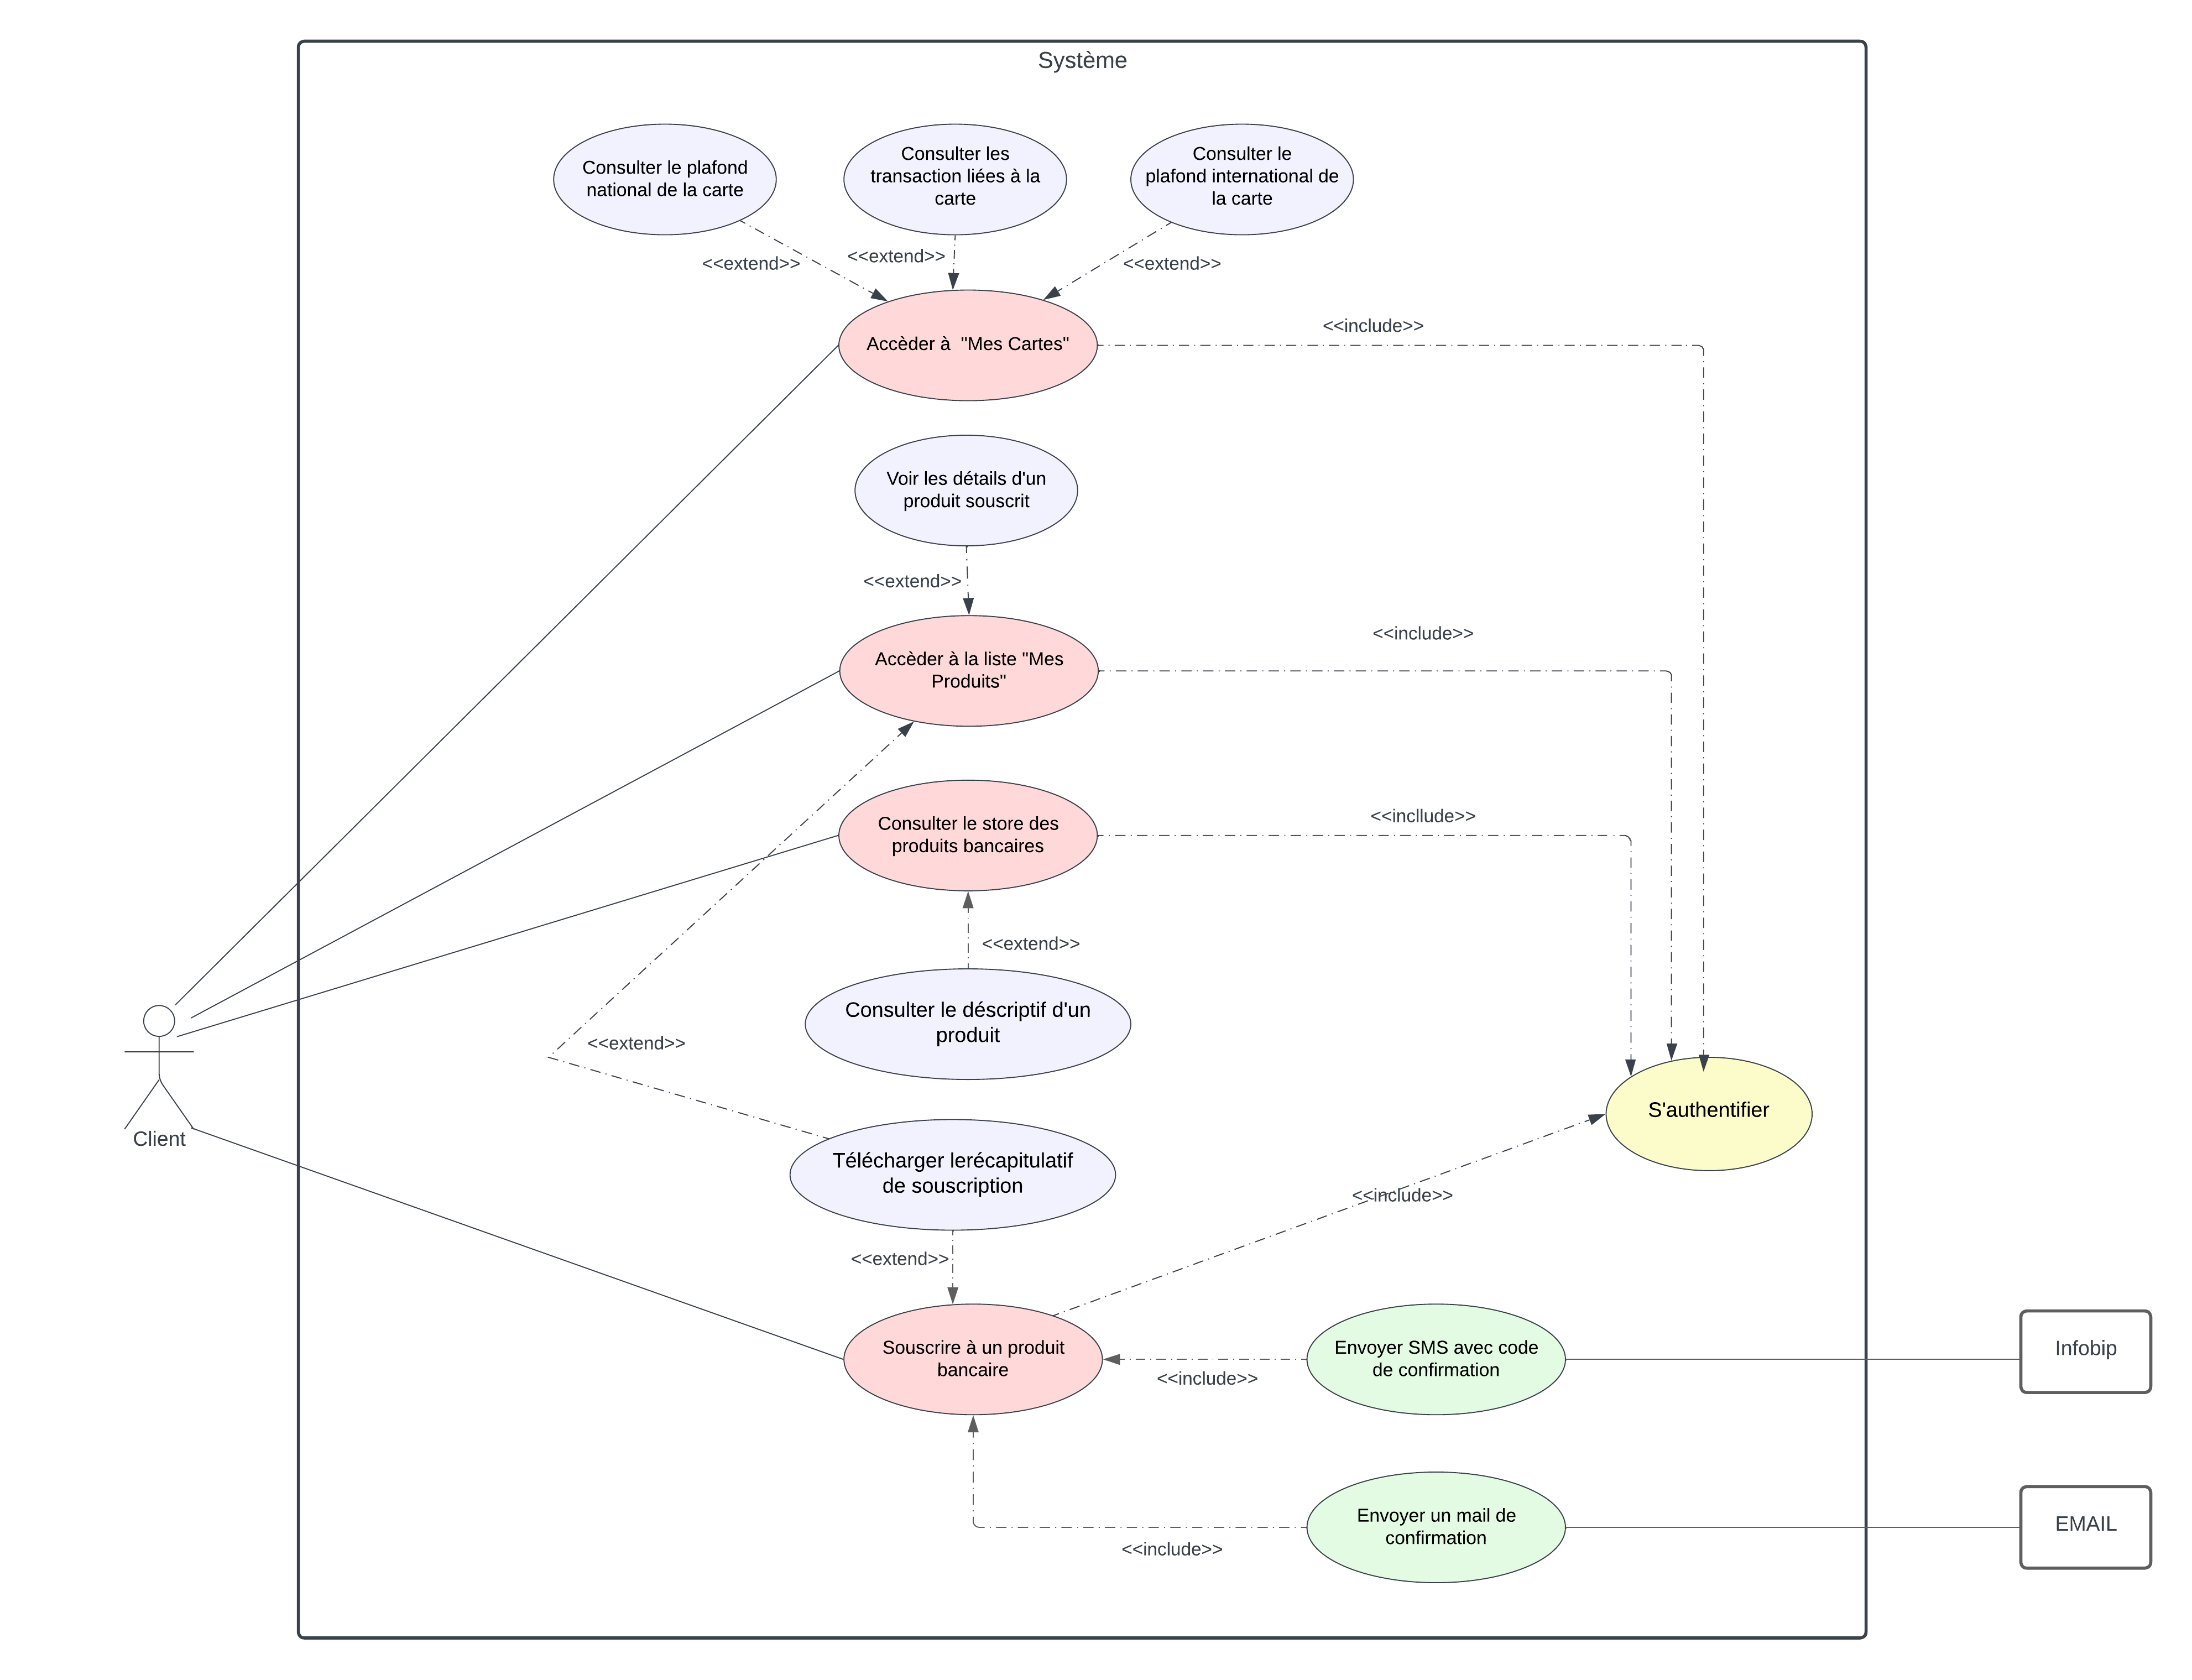
\includegraphics[width=16cm]{images/diagramms/useCase.png}
    \caption{Diagramme de cas d'utilisation}
\end{figure}
\newpage

Dans le diagramme de cas d'utilisation de notre système, nous avons les acteurs suivants :

\begin{itemize}
    \item[•] \textbf{Client :}  Représente l'utilisateur final, c'est-à-dire le client de la banque qui utilise l'application SG CONNECT pour accéder aux fonctionnalités bancaires disponibles.
    \item[•] \textbf{Infobip :} Système tiers qui joue le rôle de fournisseur de services d'envoi de SMS. Il est responsable du traitement des demandes d'envoi de SMS provenant de l'application SG CONNECT et de l'envoi des notifications SMS aux utilisateurs.
    \item[•] \textbf{EMAIL :} Système tiers qui gère l'envoi de notifications par courrier électronique aux utilisateurs. Il est utilisé pour informer les utilisateurs des opérations exécutées sur leur compte bancaire et pour partager l'historique des transactions, par exemple.
\end{itemize}

Ces acteurs interagissent avec le système SG CONNECT pour accéder aux fonctionnalités offertes et bénéficier des services bancaires à distance de manière sécurisée et pratique. Le client utilise l'application pour consulter ses comptes, effectuer des transactions, gérer ses cartes monétiques, etc. Infobip et EMAIL interviennent pour faciliter la communication avec les utilisateurs via des notifications SMS et des courriers électroniques.\\

Il est important de noter que dans ce diagramme de cas d'utilisation, le client est le principal acteur qui interagit directement avec le système, tandis que Infobip et EMAIL sont des acteurs externes qui fournissent des services de communication complémentaires.\\

\textbf{\large{Description des cas d’utilisations :}\\}

\textbf{Accéder à "Mes Cartes"} : Ce cas d'utilisation permet au client d'accéder à la liste de ses cartes monétiques associées à ses comptes bancaires. Le client peut consulter le plafond national ou international de chaque carte et afficher les transactions liées à chaque carte.\\

\textbf{Accéder à la liste "Mes Produits"} : Ce cas d'utilisation permet au client d'accéder à la liste des produits bancaires qu'il a souscrits. Le client peut voir les détails d'un produit souscrit spécifique et télécharger un récapitulatif de souscription pour référence.\\

\textbf{Consulter le store des produits bancaires} : Ce cas d'utilisation permet au client de consulter le catalogue des produits bancaires disponibles. Le client peut consulter le descriptif de chaque produit pour obtenir des informations détaillées.\\

\textbf{Souscrire à un produit bancaire} : Ce cas d'utilisation permet au client de souscrire à un produit bancaire spécifique. Le client peut télécharger un récapitulatif de la souscription pour référence. Lors de la souscription, le système envoie un SMS avec un code de confirmation en utilisant le service d'Infobip, et envoie également un mail de confirmation en utilisant le service d'EMAIL.\\

Tous les cas d'utilisation nécessitent une authentification préalable du client pour garantir la sécurité et la confidentialité des données.

\section{Conclusion}
Ce chapitre a été consacré à une étude détaillée du projet, mettant l'accent sur la spécification des besoins et leur analyse approfondie. Nous avons identifié les besoins fonctionnels et non fonctionnels du système, en nous assurant de couvrir les différentes fonctionnalités nécessaires pour répondre aux attentes des utilisateurs. Le diagramme de cas d'utilisation a permis de représenter de manière visuelle les interactions entre les acteurs et le système, en mettant en évidence les différentes fonctionnalités offertes. Cette analyse approfondie des besoins servira de base solide pour la conception de l'architecture du système, qui sera abordée dans le prochain chapitre. En concevant clairement l'architecture, nous pourrons garantir que le système répondra de manière efficace et satisfaisante aux besoins identifiés dans cette étude détaillée.
\chapter{Conception détaillée du système}
\par  Dans ce chapitre, nous entamerons la phase de conception dans le but de présenter une
solution applicative répondant aux besoins retenus. Dans cette optique, l'architecture et les diagrammes de séquence sont définis. 


\clearpage
\section{Introduction}
Le chapitre de la conception détaillée du système joue un rôle crucial dans le développement d'un projet de banque en ligne. Il s'agit d'une phase clé où nous passons de la phase de conception générale à une représentation plus spécifique et détaillée de l'architecture, des fonctionnalités et du comportement de notre application.\\

Dans ce chapitre, nous allons explorer en profondeur la conception de notre système de banque en ligne, en utilisant diverses techniques et outils de modélisation pour représenter les différents aspects du système. Nous allons examiner les principaux éléments de conception tels que l'architecture globale, les composants clés, les interactions entre les modules, ainsi que les fonctionnalités spécifiques.\\

L'objectif de cette phase de conception détaillée est de créer une base solide pour le développement de notre application. Nous allons utiliser des techniques éprouvées, telles que le diagramme de classe, les diagrammes de séquences, l'architecture en couches, les modèles de conception, et d'autres méthodes de modélisation pour représenter les différentes parties du système.

\section{Architecture logique d'UNIBANK}
Ce projet est réalisé en collaboration avec l'équipe Unibank, qui joue un rôle clé en tant que moteur BACKEND pour les différents projets au sein de la SG ABS. Unibank est une plateforme d'Open Banking innovante qui répond aux besoins digitaux des filiales de la région AFS. L'Open Banking est une initiative réglementaire qui exige des banques d'ouvrir leurs API à des services tiers, permettant ainsi le partage de données financières des clients de manière conforme et standardisée. Il fournit des orientations pour moderniser les approches bancaires et améliorer le service client.\\

Cependant, chaque banque peut adopter une approche personnalisée pour mettre en œuvre des projets adaptés à son activité. C'est dans ce contexte que la Digital Factory a développé la plateforme digitale UNIBANK. Cette plateforme permet de construire rapidement des solutions qui consomment des services CBS (ou autres) en simplifiant la complexité de ces différents services.\\

La structure de la plateforme UNIBANK est illustrée dans la figure suivante :

\begin{figure}[!h]
    \centering %
        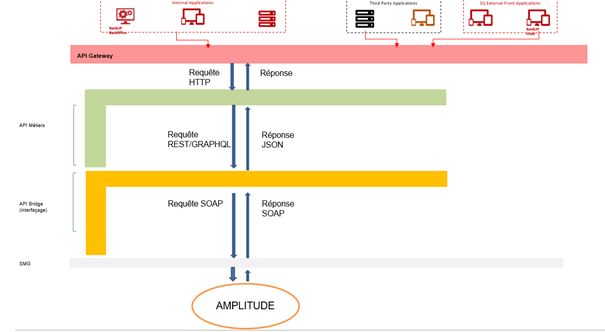
\includegraphics[width=16cm]{images/conception/architectureUNIBANK.png}
    \caption{Rôle des APIs UNIBANK dans le cadre du programme Bank-UP}
\end{figure}
\newpage

La plateforme UNIBANK est composée de trois couches distinctes :

\begin{itemize}
    \item[•] \textbf{L'API Bridge} assure une communication sécurisée avec les systèmes d'informations externes tels qu'Amplitude et Infobip, en utilisant des connecteurs. Son rôle est d'intégrer, de mapper et de traduire les données entre les APIs UNIBANK et ces systèmes externes.
    \item[•] \textbf{Les APIs métier} transforment et exploitent les données provenant du bridge ou des systèmes externes en appliquant des règles de gestion métier. Elles répondent ainsi à des besoins spécifiques des applications clientes, tels que l'affichage des comptes ou l'exécution de virements.
    \item[•] \textbf{ Les Gateways} sont des composants supplémentaires qui garantissent un accès sécurisé aux APIs UNIBANK en utilisant un mode d'authentification. Ils exposent les données provenant des APIs UNIBANK aux applications clientes.
\end{itemize}

\section{Architecture technique d'UNIBANK}
\textbf{\large{Architecture Hexagonal}\\}

Dans l'architecture technique d'UNIBANK, l'approche hexagonale a été adoptée pour préserver la logique métier, qui représente la plus grande valeur ajoutée de l'application. Cette architecture se compose de trois principales parties : le domaine métier (User Side), l'application (Business Logic) et l'infrastructure (Server Side).

\begin{figure}[!h]
    \centering %
        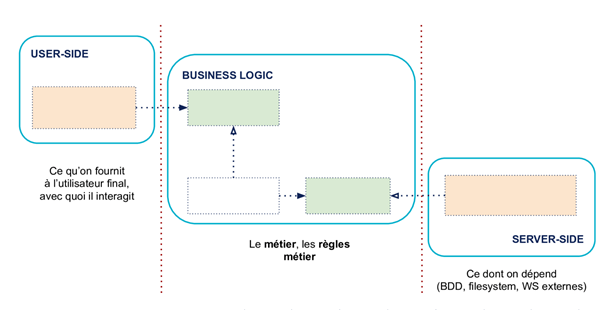
\includegraphics[width=16cm]{images/conception/hexagonal.png}
    \caption{Couches de l’architecture Hexagonale}
\end{figure}

\begin{itemize}
    \item[•] \textbf{Le domaine métier (User Side)} est le côté par lequel les utilisateurs ou les programmes extérieurs interagissent avec l'application. On y trouve le code qui gère ces interactions, tels que le code d'interface utilisateur, les routes HTTP pour une API et les sérialisations en JSON destinées à d'autres programmes qui consomment l'application.
    \item[•] \textbf{L'application (Business Logic)} est la partie centrale de l'architecture où se trouve toute la logique métier. On y retrouve le vocabulaire métier et la logique purement métier, qui résolvent le problème concret auquel l'application est dédiée. Cette partie contient la richesse et la spécificité de l'application. L'objectif est que même un expert du métier, sans compétences en développement, puisse lire le code de cette partie et identifier les incohérences éventuelles.
    \item[•] \textbf{L'infrastructure (Server Side)} regroupe les composants nécessaires au bon fonctionnement de l'application. On y trouve le code qui interagit avec la base de données, effectue des appels système de fichiers ou gère des appels HTTP vers d'autres applications. Cette partie est responsable de la mise en place de l'infrastructure technique nécessaire à l'exécution de l'application.
\end{itemize}

Au sein de la DiFa, UNIBANK a adapté cette architecture pour répondre à ses besoins techniques et fonctionnels. Toutefois, en raison de la dépendance du Bridge (connecteur externe) à un CBS externe, quelques modifications ont été apportées à l'architecture. L'accent a été mis sur deux couches principales :

\begin{itemize}
    \item[1-] \textbf{unibank-domain (Domain layer) :} Cette couche contient deux sous-projets Java :
    \begin{itemize}
        \item[-] \textbf{Platform model :} Il s'agit du socle technique du domaine, qui comprend les annotations, la gestion des permissions, la documentation, etc.
        \item[-] \textbf{Core domain :}  Ce sous-projet contient des classes Java qui représentent des besoins anticipés de l'application. Il regroupe la logique métier de la banque, divisée en trois packages :
        \begin{itemize}
            \item[•] \textbf{Base :} Ce package contient les classes POJO nécessaires pour créer une requête/réponse afin de satisfaire un besoin anticipé.
            \item[•] \textbf{Business :} Ce package gère la gestion des administrateurs et des utilisateurs.
            \item[•] \textbf{Providers :} Ce package représente la majeure partie du travail réalisé. Il contient des classes POJO utilisées par presque tous les connecteurs.
        \end{itemize}
    \end{itemize}
    \item[2-] \textbf{unibank-bridge (Application Layer)} Cette couche contient un ensemble de connecteurs, un module de configuration et un module d'exposition jouant le rôle d'adaptateur :
    \begin{itemize}
        \item[-] \textbf{Les connecteurs :} Ces modules exposent des APIs répondant à des besoins souvent techniques.
        \item[-] \textbf{Module de configuration :} Ce module gère la configuration des filiales et des connecteurs. Chaque environnement de développement dispose de sa propre configuration, soit par le biais d'un fichier de configuration, soit par l'utilisation de Vault.
        \item[-] \textbf{Module d'exposition (Adaptateur) :} Pour assurer un couplage faible, unibank a proposé ce module pour gérer la partie de la création des Beans java. Dans ce module et en se basant sur le module de configuration on peut exposer nos APIs pour n’importe
        quel connecteur.
    \end{itemize}
\end{itemize}

\begin{figure}[!h]
    \centering %
        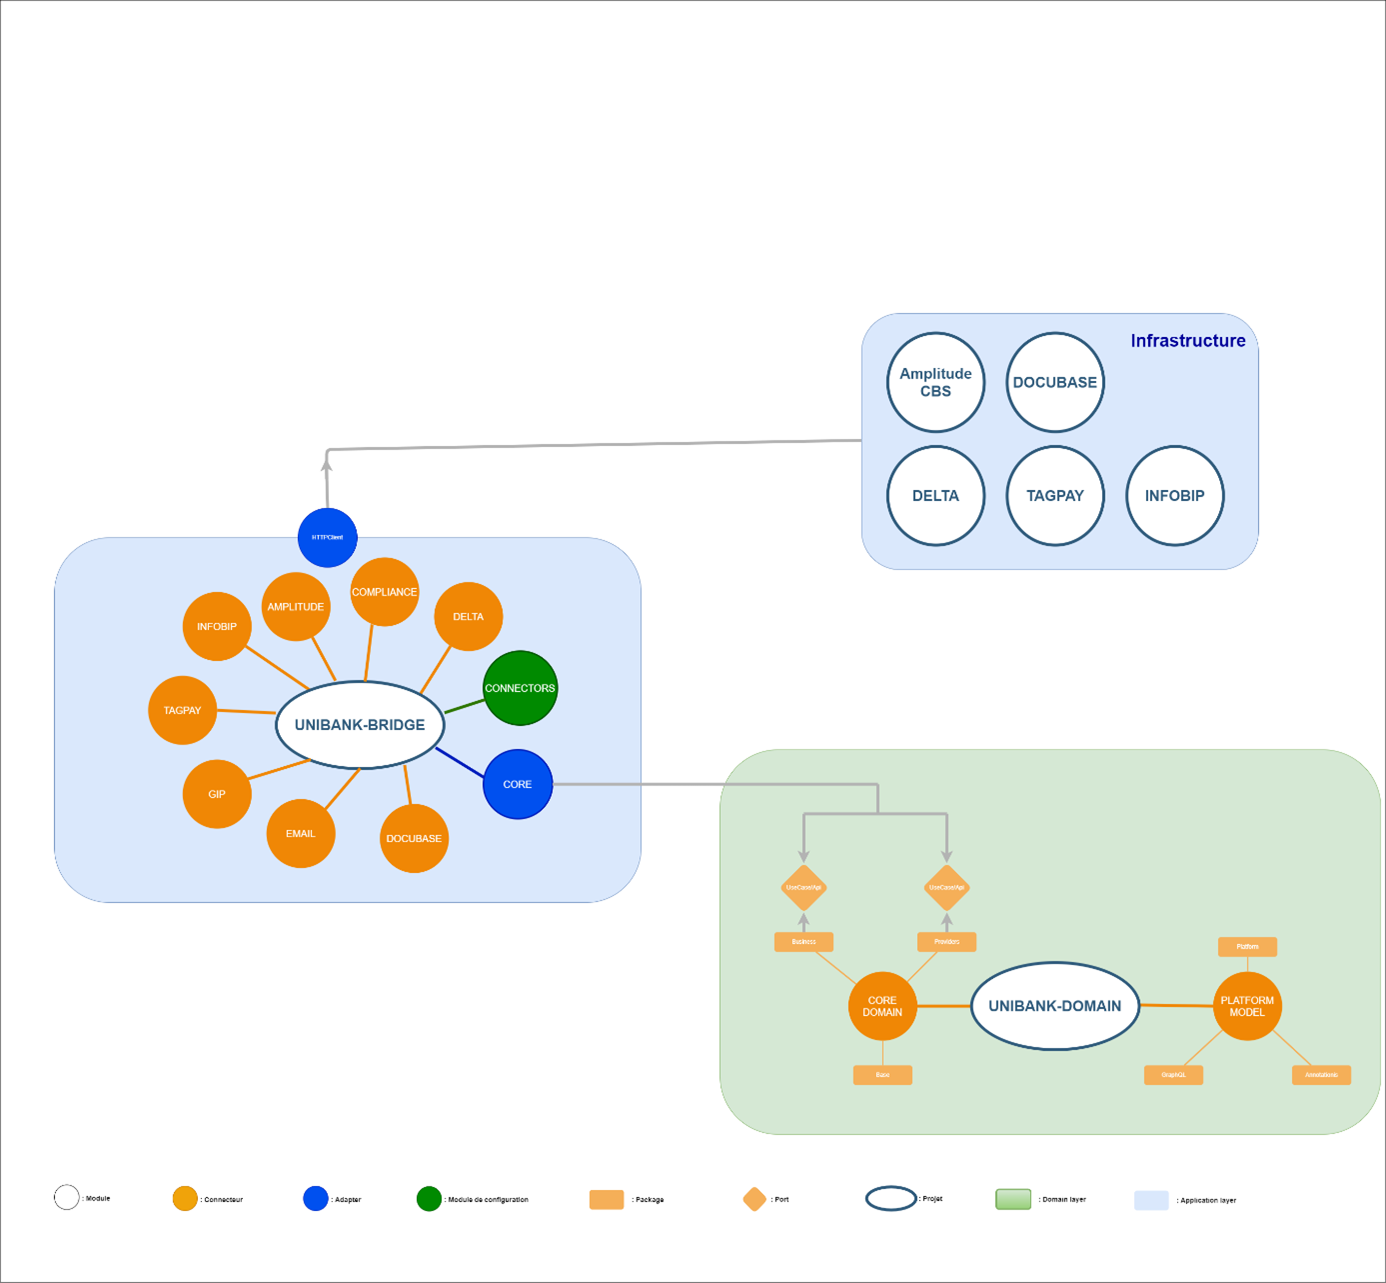
\includegraphics[width=16cm]{images/conception/architectureTechnique.png}
    \caption{Architecture technique d’UNIBANK}
\end{figure}
\newpage

\section{Technique d'Authentification/Authorisation}
Une fois que le token est généré par WSO2, il doit passer par une couche de vérification pour s'assurer de sa validité, de sa non-expiration et du type d'utilisateur qui l'utilise. Pour cela, nous utilisons un package appelé Jwt dans unibank-platform. Voici un résumé du processus de vérification des tokens :
\begin{enumerate}
    \item L'utilisateur envoie le token dans l'en-tête de la requête HTTP.
    \item En utilisant un filtre HTTP implémenté dans unibank-platform et en appliquant la méthode parseToken, nous pouvons extraire les informations de l'utilisateur :
    
    \begin{figure}[!h]
        \centering %
            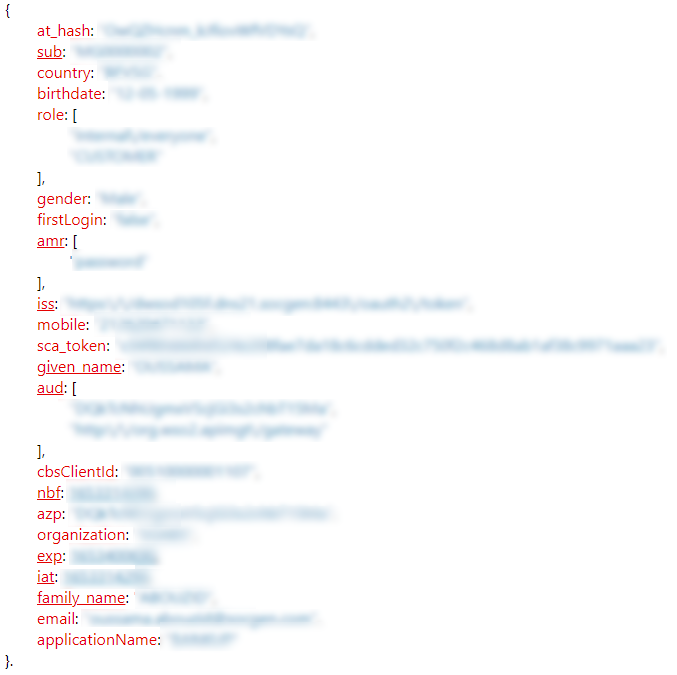
\includegraphics[width=16cm]{images/conception/exempleDeDonnees.png}
        \caption{Exemple de données d’un utilisateur en se basant sur son Token}
    \end{figure}
    \newpage

    \item La méthode parseToken permet de déchiffrer le token en utilisant l'algorithme RS256, que nous détaillerons par la suite.
    \item Après le déchiffrement du token, nous pouvons identifier l'utilisateur qui souhaite consommer l'API ainsi que ses droits.\\
\end{enumerate}

\textbf{\large{L'algorithme RS256}\\}

L'algorithme RS256 est un algorithme de cryptographie asymétrique. Cela signifie que l'émetteur du token possède une clé privée qu'il utilise pour générer la signature, tandis que le consommateur du JWT utilise une clé publique pour valider la signature. Cet algorithme est couramment utilisé pour échanger des données confidentielles sur un réseau.

\begin{figure}[!h]
    \centering %
        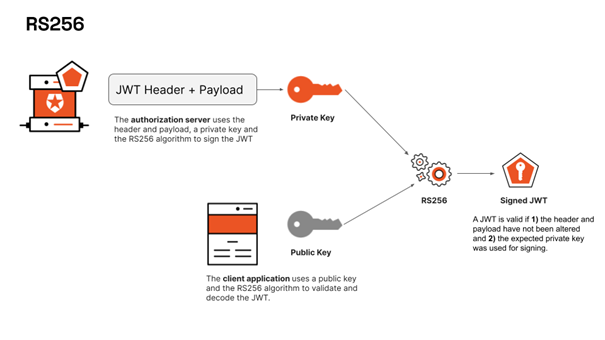
\includegraphics[width=16cm]{images/conception/algorithme.png}
    \caption{Principe d’algorithme RS256}
\end{figure}

Cet algorithme est basé sur une problématique mathématique assez célèbre, en effet supposant qu'on a p * q = n avec $n \in Z $ et p et q sont des nombres premiers, si nous savons p et q en peut déduire n, mais le contraire est très difficile.


\section{Connecteurs externes}
\textbf{\large{AMPLITUDE}\\}

\par Amplitude est un système bancaire de base (CBS) utilisé pour prendre en charge les transactions courantes d'un établissement bancaire. Les fonctionnalités bancaires de base varient en fonction du type spécifique d'établissement. Par exemple, les banques de détail ciblent les clients particuliers, tandis que les banques d'investissement traitent principalement des transactions entre institutions financières. Les systèmes bancaires de base sont souvent spécialisés dans un type spécifique d'opérations bancaires, tandis que les systèmes bancaires universels sont conçus pour prendre en charge plusieurs types de fonctions bancaires.\\

Pour répondre à ses besoins métiers, la Digital Factory utilise le CBS de Sopra, qui propose une solution robuste appelée Amplitude.\\

\textbf{\large{INFOBIP}\\}

Infobip est une entreprise leader dans le domaine des solutions de communication cloud et de messagerie omnicanal. Leur plateforme permet aux entreprises d'envoyer des messages SMS, des messages vocaux, des e-mails et d'autres types de notifications à leurs clients dans le monde entier. Infobip offre également une gamme de services de messagerie instantanée, tels que WhatsApp, Facebook Messenger et Viber, qui facilitent la communication directe avec les clients via les applications de messagerie les plus populaires.\\

\textbf{\large{EMAIL}\\}

Le courrier électronique repose sur le concept client/serveur, ce qui implique l'utilisation de deux composants : le client de messagerie (Mail User Agent : MUA), tel que Outlook, Messenger, Eudora, et le serveur de messagerie (Mail Transport Agent : MTA), tel que SendMail. Les clients de messagerie s'appuient sur un serveur de messagerie pour recevoir et envoyer des messages.\\

Dans le contexte bancaire, l'envoi d'e-mails via les API backend revêt une grande importance, car cela permet de sécuriser le traitement des données clients et de notifier en temps réel les opérations effectuées sur leur compte. Le connecteur EMAIL facilite ainsi l'envoi de courriers électroniques aux clients après une ou plusieurs opérations bancaires.

\section{Architecture Monorepo de la partie Front-end}
Dans le projet de banque en ligne, l'architecture monorepo a été choisie pour regrouper les différentes applications, à savoir le développement web, mobile et une autre application spécifique. Cette approche consiste à centraliser l'ensemble du code source dans un seul référentiel, offrant ainsi une vision unifiée de toutes les applications.\\

L'adoption de l'architecture monorepo présente plusieurs avantages. Tout d'abord, elle favorise la collaboration entre les équipes de développement en simplifiant le partage de code entre les différentes plates-formes. Les développeurs peuvent travailler plus efficacement en réutilisant les composants et les fonctionnalités communes, ce qui accélère le processus de développement et garantit une cohérence globale.\\

De plus, l'architecture monorepo facilite la maintenance et les mises à jour du système. Les modifications apportées à une partie de l'application peuvent être rapidement propagées à l'ensemble du système, ce qui réduit les risques d'incohérence et améliore la stabilité globale de l'application.\\

En comparaison, l'approche multi-repo, qui consiste à maintenir des référentiels distincts pour chaque application ou composant, présente une séparation plus stricte entre les différents éléments. Bien qu'elle puisse offrir une isolation plus granulaire et faciliter la gestion indépendante des applications, elle peut également entraîner une duplication de code et rendre le partage de fonctionnalités plus complexe.

\begin{figure}[!h]
    \centering %
        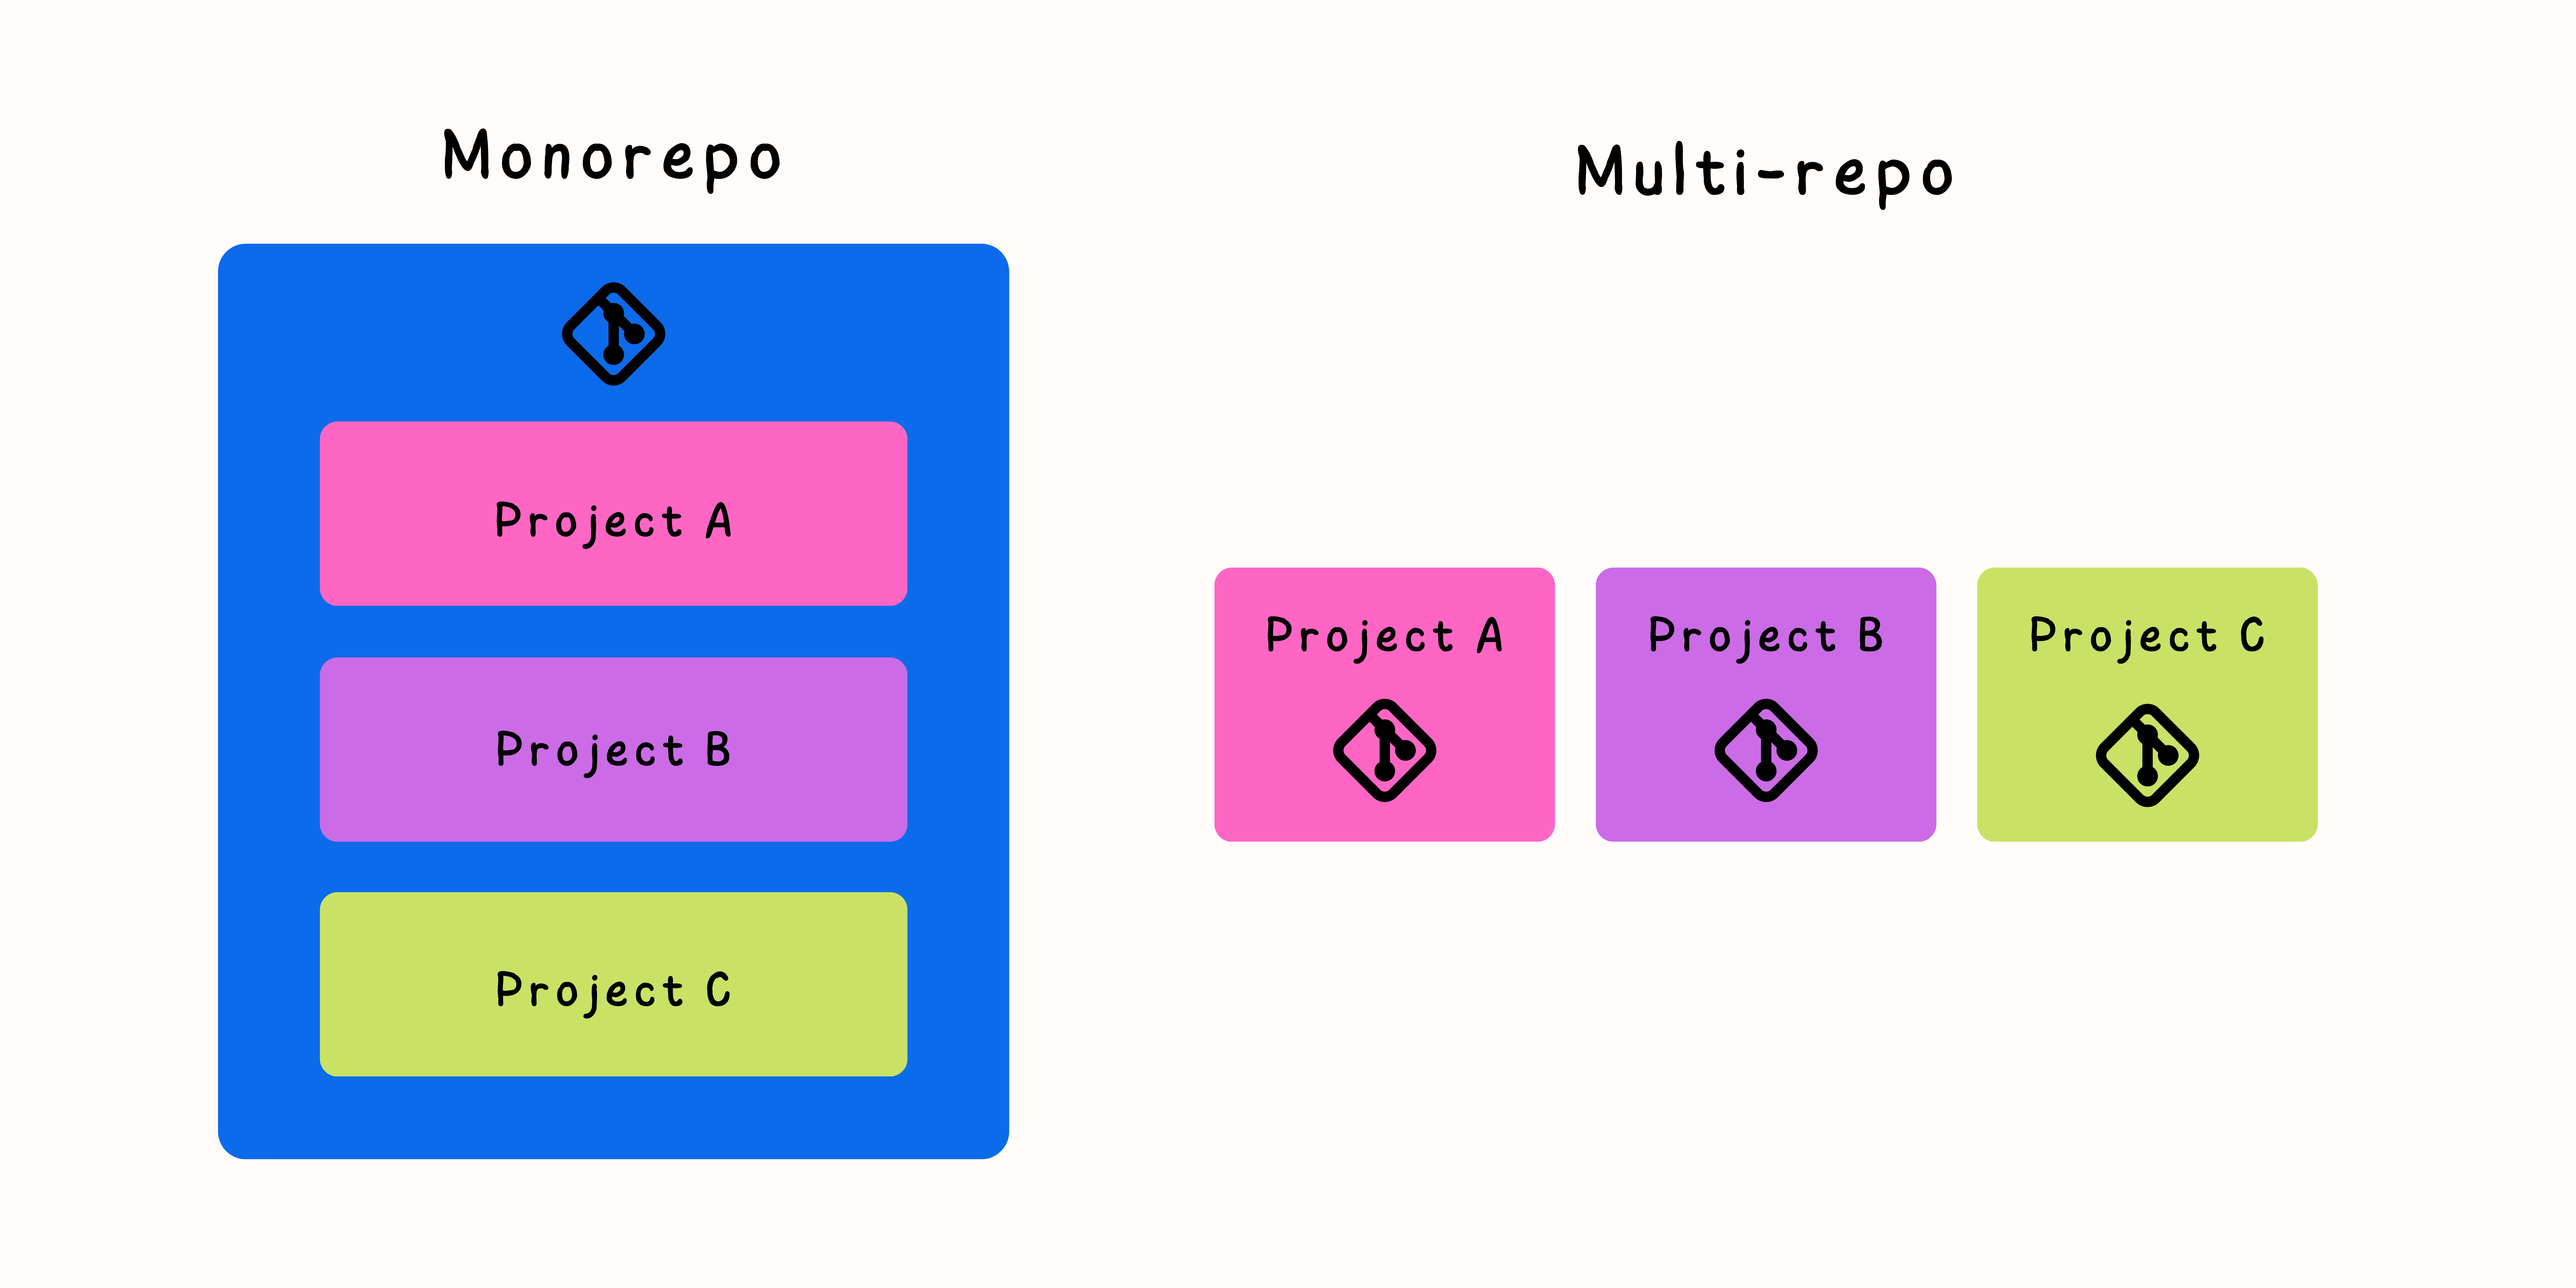
\includegraphics[width=16cm]{images/conception/monoRepo.png}
    \caption{Comparaison entre l’architecture monorepo et multi-repo}
\end{figure}

Dans l'architecture détaillée du Front-End de l'application SG CONNECT, représentée dans la figure suivante :
\begin{figure}[!h]
    \centering %
        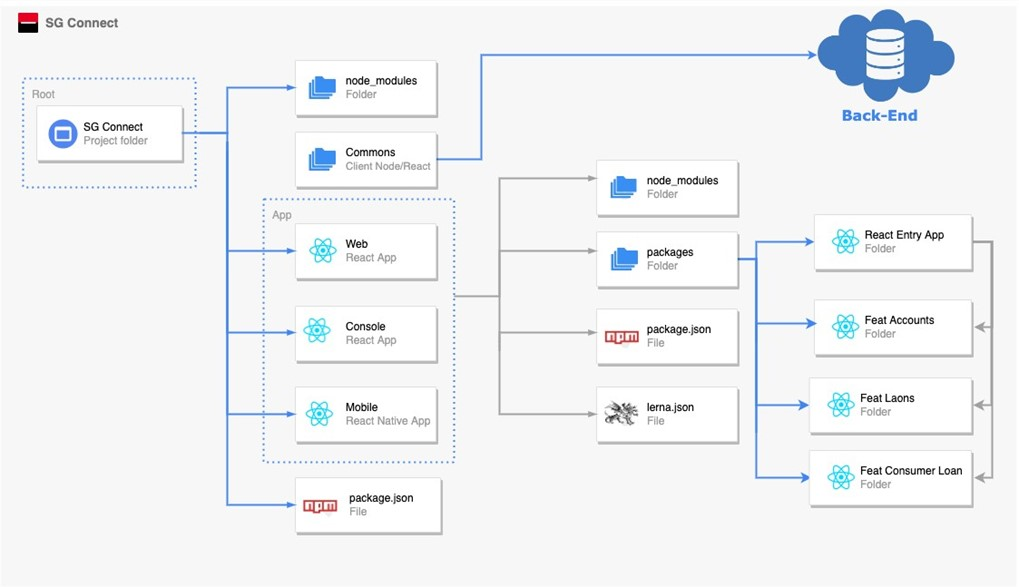
\includegraphics[width=14cm]{images/conception/architectureFRONT.jpg}
    \caption{Architecture Front-End du SG CONNECT}
\end{figure}

nous avons trois applications FRONT regroupées dans un monorepo. Ces applications servent les clients de la banque de détail des filiales AFS. Les trois applications sont les suivantes :

\begin{itemize}
    \item[•] Une application mobile compatible avec les plateformes Android et iOS.
    \item[•] Une application web pour une expérience utilisateur conviviale via les navigateurs.
    \item[•] Une application web console backoffice destinée aux gestionnaires afin de consulter les demandes des clients et gérer les opérations internes.
\end{itemize}

Cette architecture monorepo permet de maximiser l'efficacité de développement tout en assurant la cohérence et la stabilité de l'ensemble du système. Les équipes de développement peuvent travailler de manière collaborative, partager efficacement le code et garantir une expérience utilisateur homogène sur les différentes plates-formes.

\section{Approche Multitenant}
L'approche multitenant a été choisie afin d'éviter la duplication de code spécifique à chaque entité et de gérer efficacement les multiples clients ou filiales au sein d'une seule instance de l'application. Cette approche permet de maintenir l'isolation des données, des configurations et des personnalisations propres à chaque locataire (tenant). Une alternative à cette approche est le modèle \textbf{single tenant}, où chaque filiale dispose d'une instance dédiée de l'application avec ses propres configurations.\\

Pour simplifier la gestion des filiales, un fichier de configuration spécifique à chaque tenant, appelé \textbf{tenantconfig}, est utilisé dans le cadre de l'approche multitenant. Ce fichier contient les paramètres, les valeurs et les personnalisations propres à chaque filiale. Il permet de définir des fonctionnalités spécifiques activées ou désactivées, des règles d'accès, des paramètres de personnalisation de l'interface utilisateur et d'autres configurations uniques pour chaque entité.\\

Comparativement, le modèle \textbf{single tenant} nécessiterait la création et la maintenance de différentes instances de l'application pour chaque filiale, ce qui entraînerait une complexité accrue et une duplication des efforts de développement et de maintenance. En utilisant l'approche multitenant avec un fichier \textbf{tenantconfig}, il est possible de centraliser la gestion des différentes filiales tout en permettant une personnalisation spécifique à chaque entité. Cela favorise une approche plus efficace et évolutive pour le développement et la maintenance de l'application dans un environnement multitenant.
\begin{figure}[!h]
    \centering %
        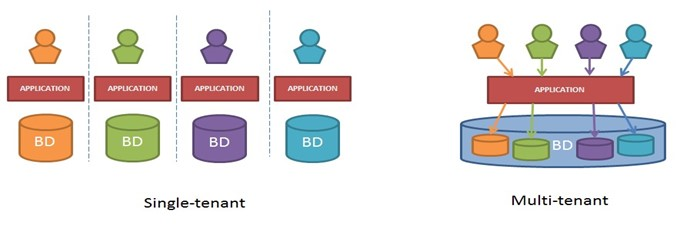
\includegraphics[width=14cm]{images/conception/teant.jpg}
    \caption{Comparaison entre l’approche single tenant et multitenant}
\end{figure}

\section{Feature Flagging}
Le \textbf{Feature Flagging} est une approche qui permet de gérer les fonctionnalités de manière flexible. Les fonctionnalités peuvent être activées ou désactivées dynamiquement en fonction des besoins et des paramètres définis. Cette approche nous offre la possibilité de tester et de déployer progressivement de nouvelles fonctionnalités, ce qui réduit les risques potentiels et garantit une meilleure qualité et stabilité du système.\\

En utilisant le "Feature Flagging", nous pouvons limiter l'impact des changements en activant les fonctionnalités uniquement pour un groupe restreint d'utilisateurs ou pour des tests internes, avant de les rendre accessibles à tous. Cela nous permet de contrôler l'exposition des nouvelles fonctionnalités et de recueillir des commentaires et des données de manière contrôlée.\\

De plus, le \textbf{Feature Flagging} offre une gestion facile des fonctionnalités en fonction des besoins spécifiques des filiales. En activant ou désactivant les drapeaux appropriés, nous pouvons personnaliser l'expérience utilisateur pour chaque filiale en leur offrant des fonctionnalités spécifiques ou en adaptant des fonctionnalités existantes selon leurs exigences. Cela nous permet de répondre aux besoins uniques de chaque filiale sans nécessiter des développements séparés pour chaque cas.
\begin{figure}[!h]
    \centering %
        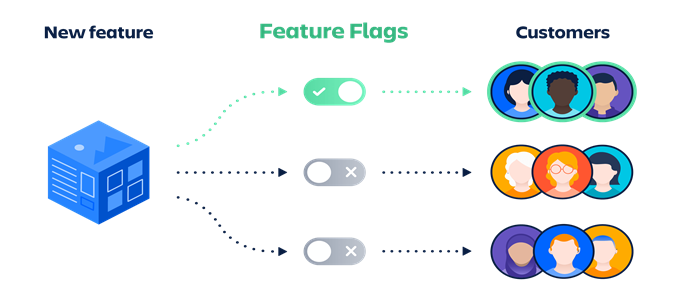
\includegraphics[width=14cm]{images/conception/flagging.png}
    \caption{Feature flagging}
\end{figure}

\section{Diagramme de classes}
Le diagramme de classes montre la structure interne du système. Il permet de fournir une
représentation abstraite des objets du système, qui vont interagir ensemble pour réaliser les cas
d’utilisation, il faut noter que ce diagramme ne présente pas toutes les classess du système, mais il présente les classes utilisées dans le projet.\\
\begin{figure}[!h]
    \centering %
        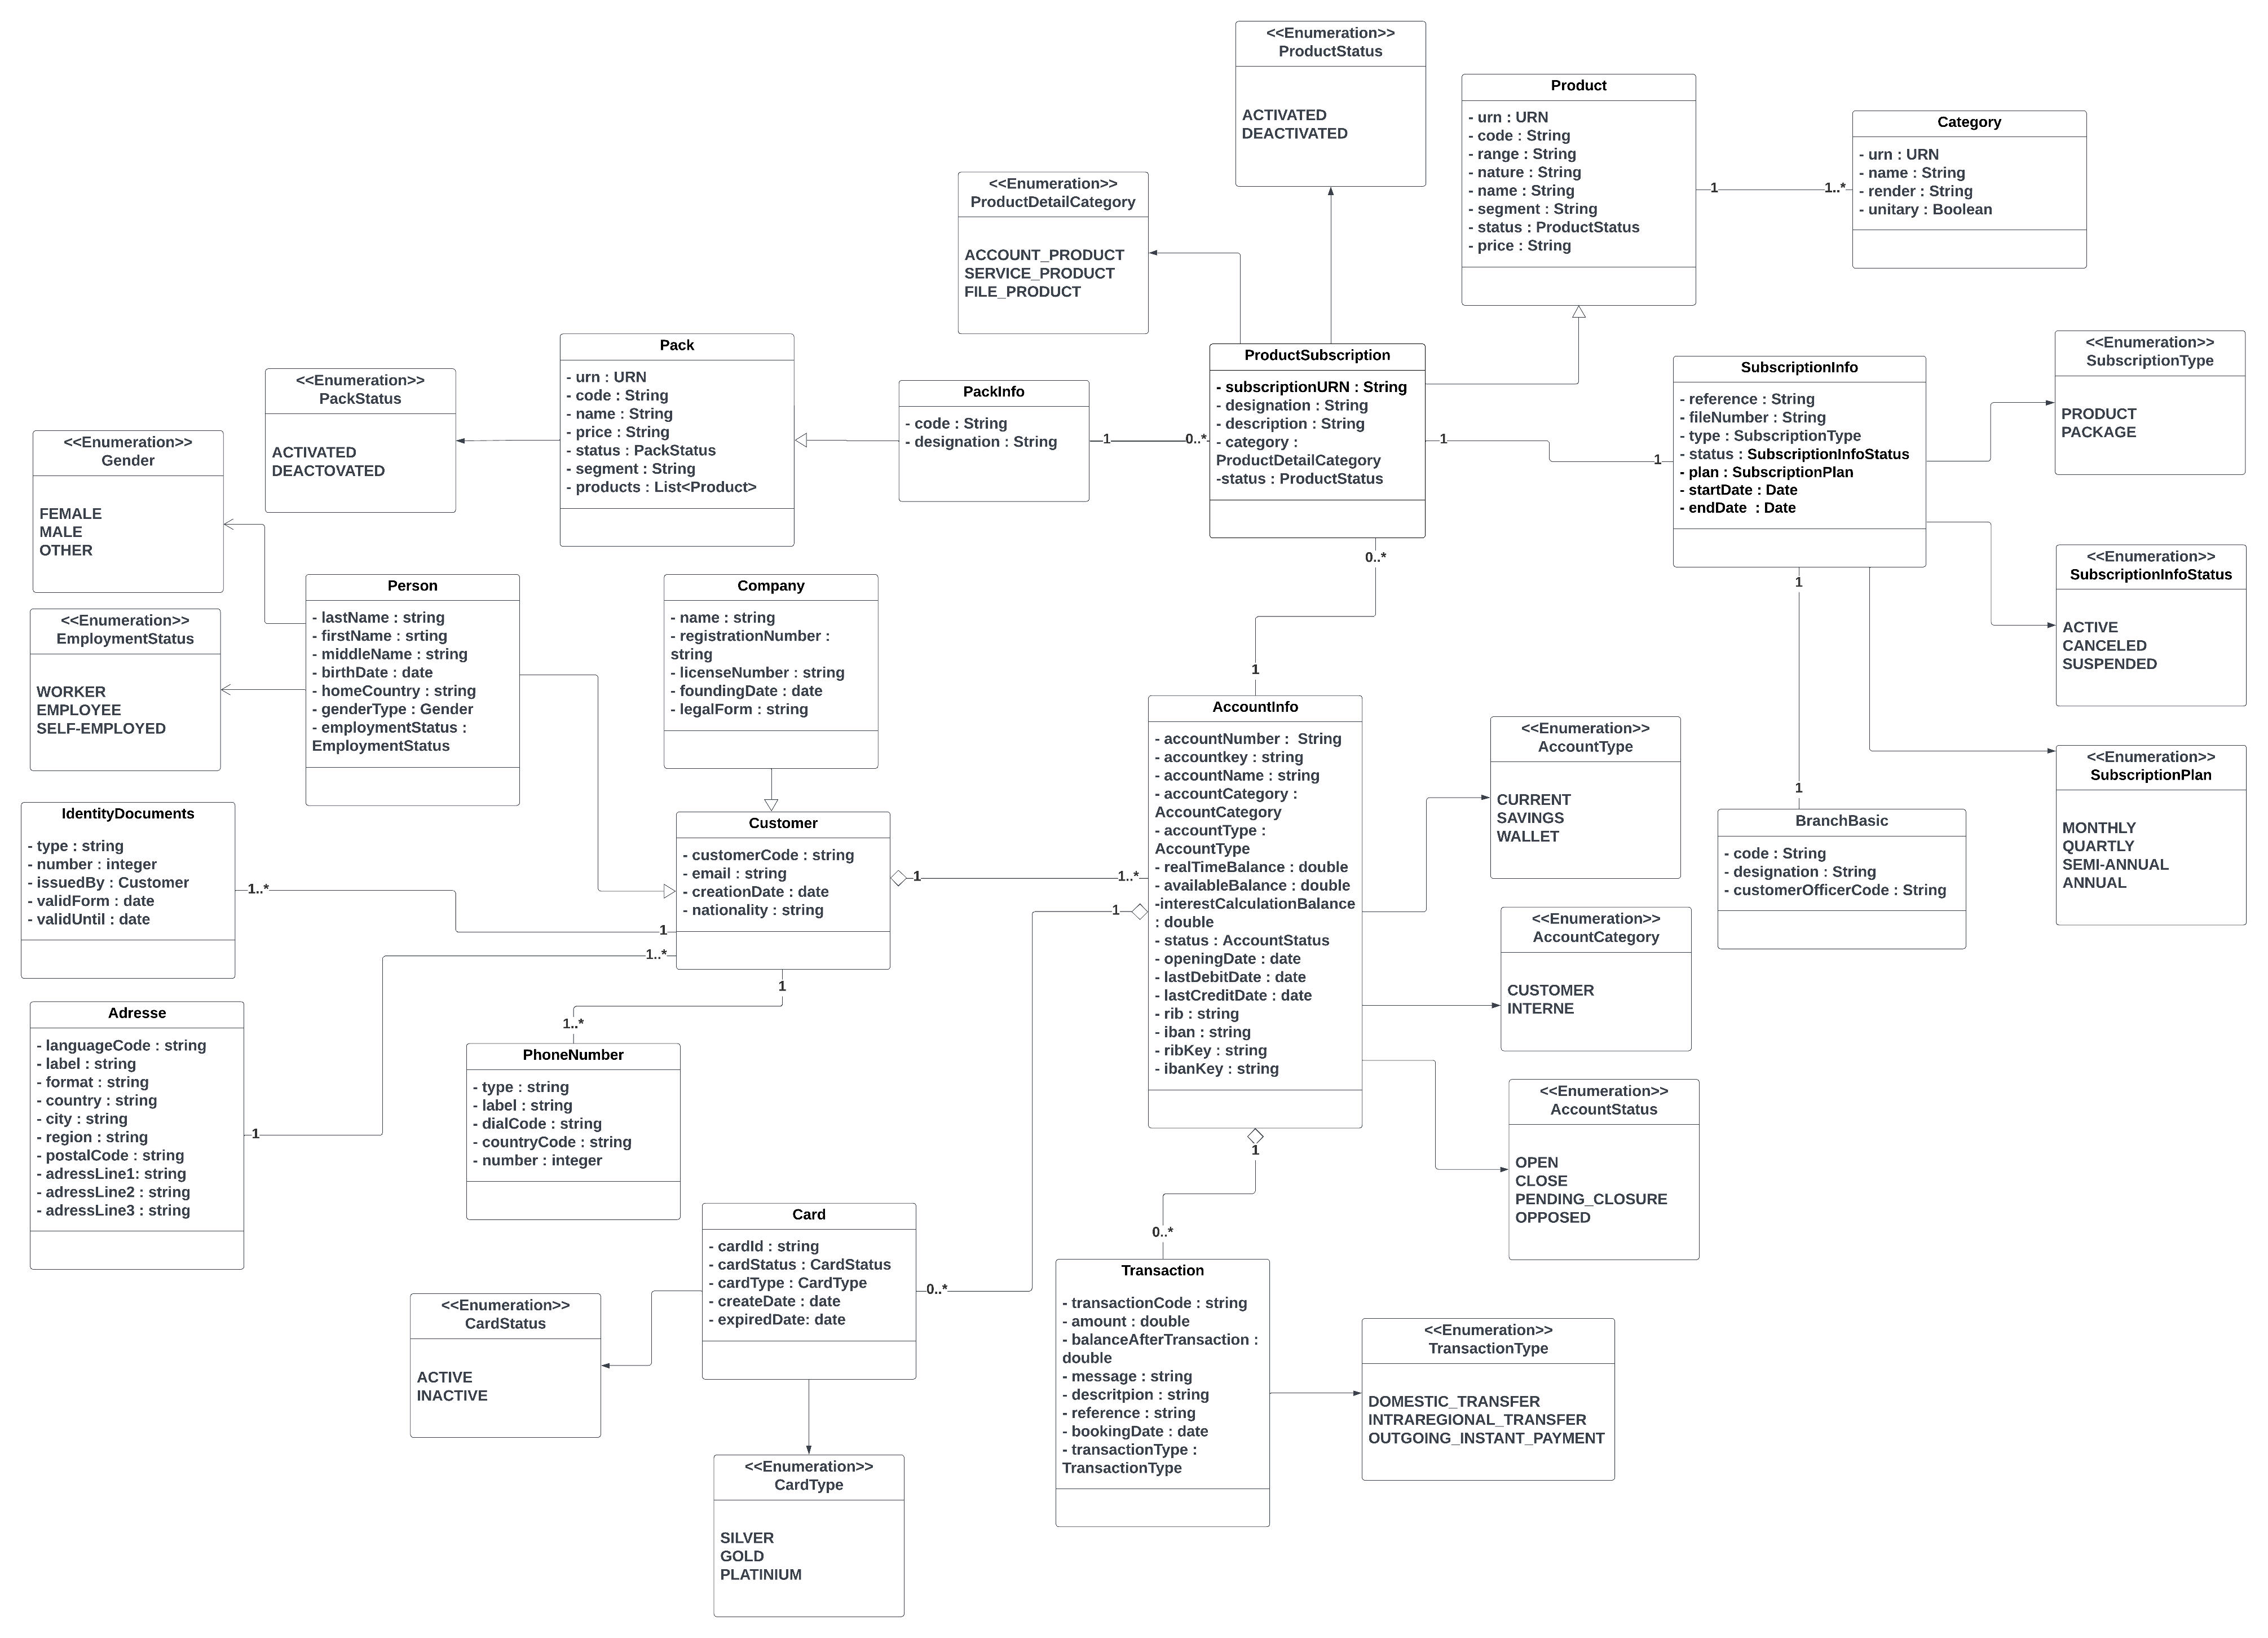
\includegraphics[width=16cm]{images/conception/diagramme_classe.png}
    \caption{Diagramme de classe}
\end{figure}

\section{Diagrammes de séquences}
\subsection{Scénario de consultation des cartes}
\begin{figure}[!h]
    \centering %
        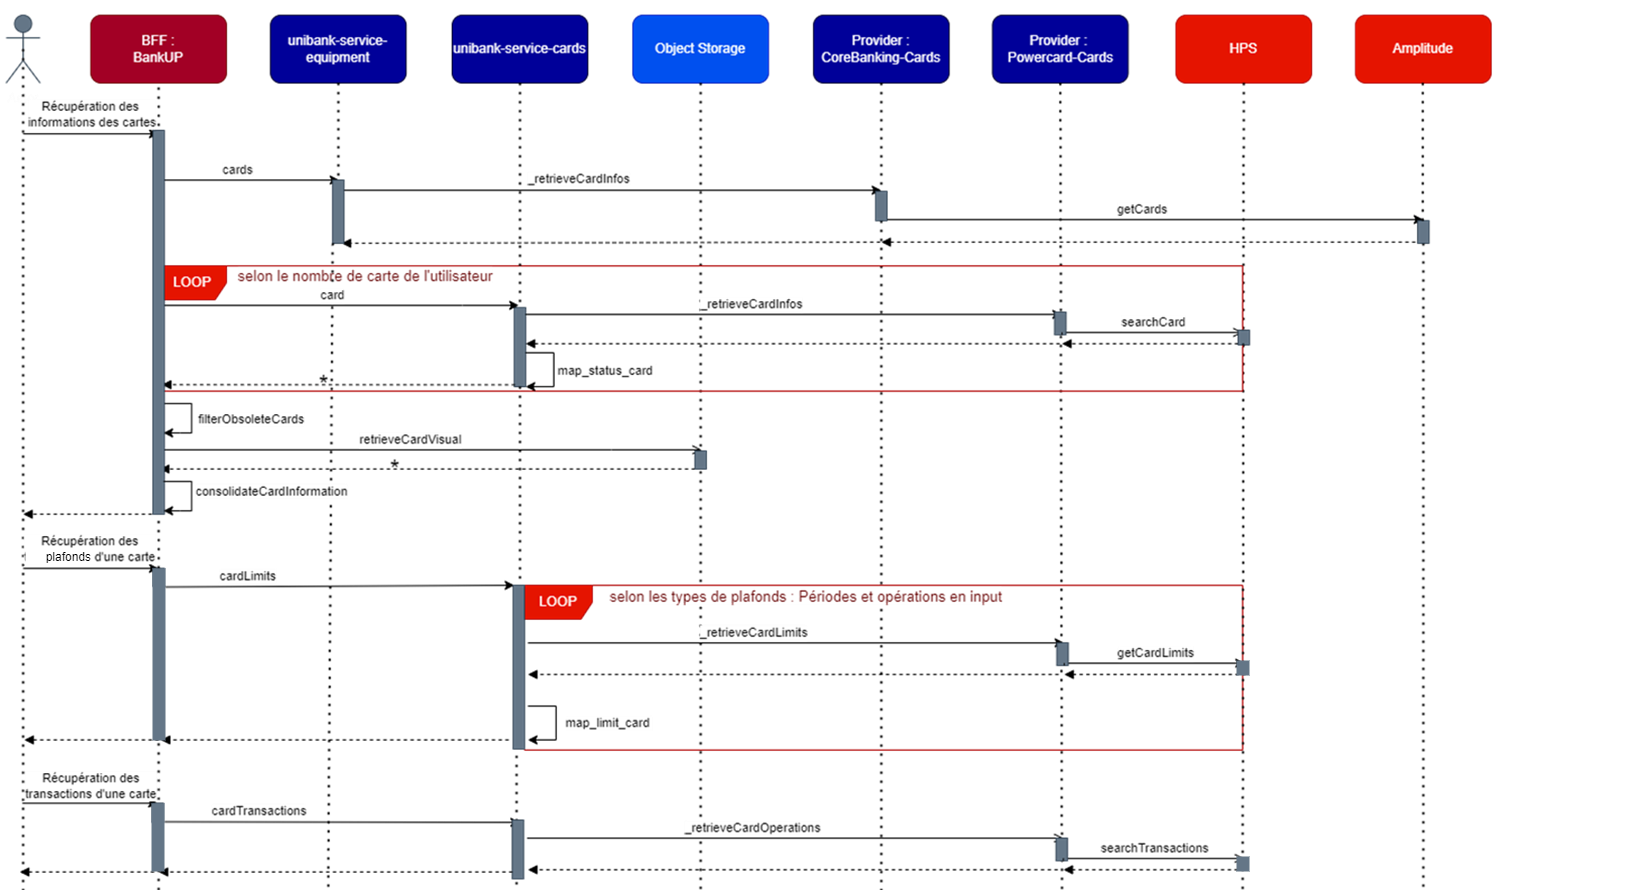
\includegraphics[width=14cm]{images/conception/sequence_cards2.png}
    \caption{Diagramme de séquence d'affichage des cartes, des plafonds et des transactions}
\end{figure}
 
Le diagramme de séquence illustre le scénario de consultation des cartes dans l'interface SG CONNECT. L'utilisateur initie la demande de récupération des informations des cartes via l'interface utilisateur. Pour obtenir les cartes, l'application utilise le service "Unibank Service Equipment" qui agit comme un pont entre l'interface utilisateur et le système bancaire central. Ensuite, le provider "Corebanking-cards" est sollicité pour obtenir les informations spécifiques liées à chaque carte. Cela se fait en utilisant l'API "getCards" fournie par le système bancaire central et en passant par le connecteur "Amplitude" qui assure la communication entre l'application et le système bancaire.\\
Une fois que les informations des cartes sont récupérées, l'application effectue un loop sur le nombre de cartes obtenues. Pendant ce processus, les statuts des cartes sont analysés et adaptés si nécessaire pour répondre aux exigences de l'équipe front-end. Plus précisément, les cartes obsolètes sont filtrées et exclues du résultat final.\\
Une fois les cartes filtrées, l'application peut visualiser et afficher les cartes du client dans l'interface SG CONNECT. Cette étape permet à l'utilisateur de consulter les détails et les informations relatives à chaque carte monétique.\\

Dans le scénario de récupération des plafonds des cartes, l'utilisateur initie la demande via l'interface front du SG CONNECT. Étant donné que nous avons déjà passé par l'étape précédente de récupération des cartes, nous pouvons passer directement à la récupération des plafonds.\\
L'application effectue un loop dans le service "Unibank Service Cards" en fonction du type de plafond, des périodes et des opérations spécifiées par l'utilisateur. En utilisant le provider "Powercard-cards" et l'API "getCardLimits" sur HPS, les plafonds des cartes sont récupérés.\\
Cependant, les données des plafonds peuvent être présentées de manière inhabituelle ou nécessiter une adaptation pour répondre aux besoins de l'application. Par conséquent, un mapping des données est effectué afin de les rendre compatibles avec le format et les exigences de l'interface utilisateur. Cette étape d'adaptation permet d'obtenir les plafonds des cartes dans un format approprié qui sont visualiser et afficher dans l'interface SG CONNECT.\\

Dans le scénario de récupération des transactions liées aux cartes, l'utilisateur initie la demande après avoir déjà obtenu les données des cartes. La demande est ensuite transmise au service "Unibank Service Cards", qui interagit avec le provider "Powercard-cards". En utilisant l'API "searchTransactions" sur HPS, les transactions liées aux cartes sont récupérées.\\
Le processus de récupération des transactions est relativement simple. Après l'initialisation de la demande par l'utilisateur, les étapes suivantes consistent en une séquence de requêtes et de récupération de données. L'interaction entre les différents composants de l'application permet d'obtenir les transactions spécifiques aux cartes sélectionnées.\\
Une fois les transactions récupérées, elles sont affichées à l'utilisateur, lui permettant ainsi de visualiser et de consulter les détails des transactions associées à ses cartes.

\newpage
\subsection{Scénario de consultation des produits}
\begin{figure}[!h]
    \centering %
        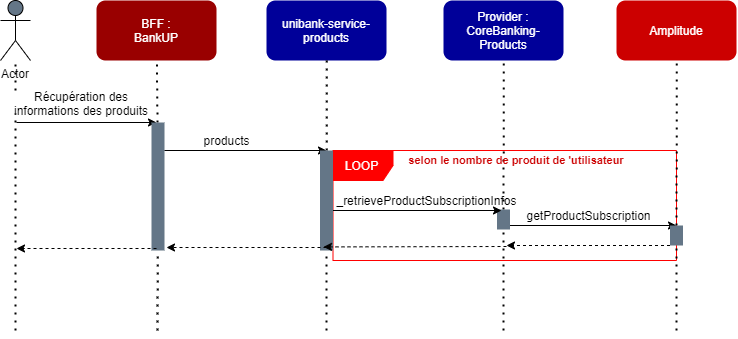
\includegraphics[width=14cm]{images/conception/sequence_products.png}
    \caption{Diagramme de séquence de consultation des produits}
\end{figure}
Dans le scénario de consultation des produits souscrits, l'utilisateur initie la demande de récupération des informations relatives aux produits auxquels il est souscrit. La demande est envoyée vers le service "Unibank Service Products", qui effectue un parcours (loop) pour récupérer tous les produits associés à l'utilisateur via le provider "Corebanking-Products".\\
En utilisant l'API "getProductsSubscription" sur Amplitude, les informations détaillées des produits sont obtenues. Une fois récupérées, ces informations sont affichées à l'utilisateur, lui permettant ainsi de visualiser et de consulter les produits auxquels il est souscrit.
\newpage

\subsection{Scénario de souscription à un produit}
\begin{figure}[!h]
    \centering %
        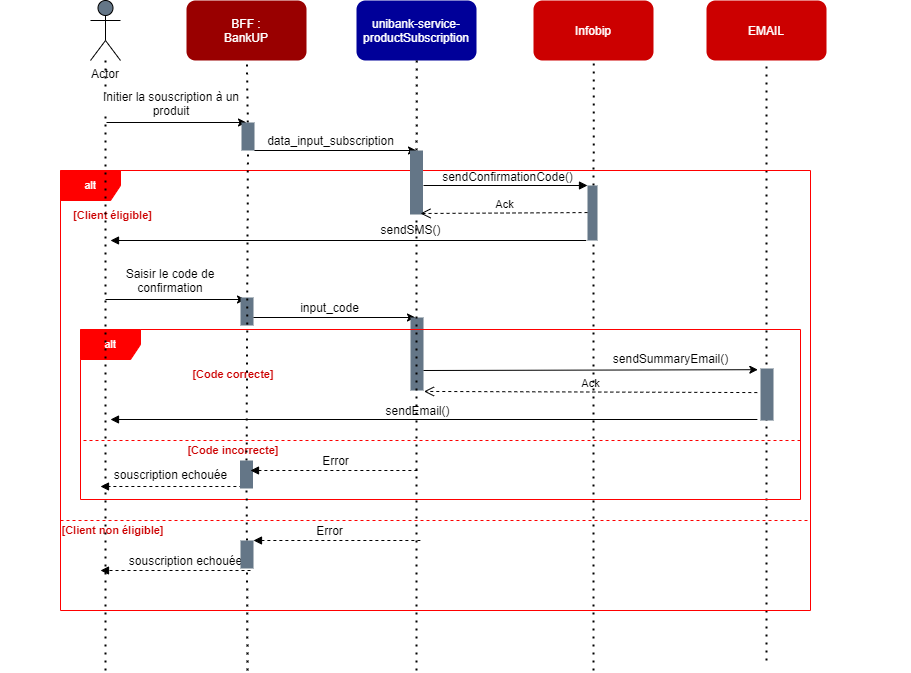
\includegraphics[width=14cm]{images/conception/sequence_souscription.png}
    \caption{Diagramme de séquence de souscription à un produit}
\end{figure}
Dans le scénario de souscription à un produit, l'utilisateur initie la souscription en fournissant certaines informations via l'interface utilisateur de SG CONNECT. Ces informations sont transmises au service "Unibank Service Product Subscription".\\
Si le client est éligible à la souscription, une demande est envoyée à "Infobip" pour l'envoi d'un code de confirmation par SMS. Le code est ensuite envoyé à l'utilisateur qui le saisit dans l'interface utilisateur de SG CONNECT.\\
Le code de confirmation est ensuite vérifié par le service "Unibank Service Product Subscription". Si le code est correct, une demande est envoyée au service "EMAIL" pour l'envoi d'un e-mail récapitulatif de la souscription à l'utilisateur. L'e-mail est alors envoyé à l'utilisateur avec les détails de sa souscription.\\
En revanche, si le code de confirmation est incorrect, le service "Unibank Service Product Subscription" renvoie une erreur qui est affichée à l'utilisateur via l'interface utilisateur de SG CONNECT. De même, si le client n'est pas éligible à la souscription, une erreur est renvoyée par le service vers l'interface utilisateur de SG CONNECT pour être affichée à l'utilisateur.

\section{Conclusion}
Au cours de ce chapitre, nous avons examiné en détail l'architecture monorepo du front-end, l'architecture hexagonale pour la logique métier, l'approche technique d'UNIBANK avec les couches du domaine et de l'application, la technique d'authentification/autorisation avec l'utilisation de JWT et l'algorithme RS256, l'approche multitenant pour gérer les différentes filiales, ainsi que le feature flagging pour activer ou désactiver dynamiquement les fonctionnalités et enfin le diagramme de classe et les diagrammes de séquences.\\
Dans le prochain chapitre, nous aborderons la réalisation et la mise en œuvre de notre application.
\chapter{Réalisation et mise en oeuvre}
\par  Dans ce chapitre, nous aborderons la phase de réalisation et de mise en œuvre de notre projet. Nous nous concentrerons sur l'implémentation concrète de l'application, en mettant en place les différentes fonctionnalités et en développant les interfaces essentielles. Nous détaillerons les choix technologiques effectués, les outils et les frameworks utilisés, ainsi que les bonnes pratiques de développement. Ce chapitre marque une étape cruciale dans la concrétisation de notre vision, où nous passerons de la conception à la création d'un produit fonctionnel et utilisable.

\clearpage

\section{Introduction}
Après avoir effectué une étude détaillée du projet et défini les besoins et les spécifications, nous entrons maintenant dans la phase de concrétisation. Ce chapitre se concentre sur la réalisation effective du système en utilisant les technologies et les outils appropriés.\\

Nous présenterons ici les différentes interfaces et fonctionnalités que nous avons développées, en mettant l'accent sur leur conception ergonomique, leur convivialité et leur adaptabilité aux différents environnements (desktop, tablette, mobile) ainsi qu'aux différentes versions linguistiques (français, anglais). Nous décrirons également les outils de développement, de test et de documentation que nous avons utilisés pour assurer la qualité du système.\\

Ensuite, nous aborderons les aspects de déploiement et d'environnements d'exécution du système. Nous décrirons les différents environnements adoptés, tels que l'environnement local pour le développement et les tests, l'environnement de développement, l'environnement d'homologation fonctionnelle, l'environnement d'homologation technique et enfin l'environnement de production. Chaque environnement joue un rôle spécifique dans la validation, la vérification et la préparation du système pour une utilisation réelle par les utilisateurs.\\

Puis, nous explorerons la phase de qualification, au cours de laquelle nous avons réalisé différents tests pour garantir la qualité et la fiabilité du système. Les tests end-to-end, les tests fonctionnels et les tests de non-régression ont été exécutés pour valider le fonctionnement global du système, la conformité des fonctionnalités aux exigences spécifiées et l'absence de régressions lors des modifications.\\

Enfin, nous mettons l'accent sur les perspectives futures pour une évolution continue du système de banque en ligne.
\section{Outils et technologies}
\subsection{Outils de Conception}
\subsection*{Figma}
Figma est un outil de conception d'interface utilisateur (UI) et d'expérience utilisateur (UX) largement utilisé dans notre projet. Il offre une plateforme collaborative et basée sur le cloud qui permet à notre équipe de travailler de manière transparente sur la création, la visualisation et la modification des maquettes et des prototypes. Grâce à ses fonctionnalités avancées, Figma facilite la création de designs interactifs, la gestion des composants réutilisables et la collaboration en temps réel entre les membres de notre équipe. De plus, l'utilisation de Figma comme outil central de conception nous permet de créer des interfaces utilisateur esthétiques et intuitives tout en favorisant une collaboration efficace entre les designers et les développeurs.
% \begin{figure}[!ht]
%     \centering %
%         
\includegraphics[height=2cm]{images/logos/figma.png}
%     \caption{Logo de Figma}
% \end{figure}

\subsection{Outils de Développement }
\subsection*{React.js}
Pour la réalisation de l'application de banque en ligne, nous avons opté pour la technologie React.js en tant que principal framework de développement. React.js est une bibliothèque JavaScript largement adoptée pour la création d'interfaces utilisateur interactives et réactives. Son approche basée sur les composants permet de diviser l'interface en éléments réutilisables, ce qui facilite la gestion du code et favorise un développement efficace. Grâce à sa virtual DOM (Document Object Model), React.js optimise les mises à jour de l'interface en minimisant les modifications réelles apportées à la page, ce qui améliore les performances globales de l'application. De plus, React.js s'intègre facilement avec d'autres bibliothèques ou frameworks, ce qui nous offre une flexibilité accrue dans le choix des outils complémentaires. L'utilisation de React.js dans notre projet nous permet de développer une application réactive, modulaire et performante, offrant ainsi une expérience utilisateur fluide et agréable.
% \begin{figure}[!ht]
%     \centering %
%         
\includegraphics[height=2cm]{images/logos/react.png}
%     \caption{Logo de React.js}
% \end{figure}

\subsection*{React Native}
React Native est un framework open source basé sur React, la bibliothèque JavaScript de Facebook, qui permet de créer des interfaces utilisateur pour les plateformes mobiles. Il offre aux développeurs la possibilité d'utiliser les fonctionnalités natives d'Android et iOS dans le développement d'applications. Grâce à React Native, il est possible d'accéder aux composants et API natifs de chaque plateforme, offrant ainsi une expérience utilisateur authentique et optimisée.
% \begin{figure}[!ht]
%     \centering %
%         
\includegraphics[height=2cm]{images/logos/reactNative.png}
%     \caption{Logo de React Native}
% \end{figure}

\subsection*{Styled Components}
Styled Components est une bibliothèque de CSS in JS qui offre une approche basée sur les composants pour la création de styles dans nos applications. Cette bibliothèque permet de définir des styles de manière plus modulaire et réutilisable, en encapsulant le style dans des composants.\\

Avec Styled Components, nous pouvons créer des styles dynamiques en utilisant des template strings qui nous permettent d'incorporer des variables et de passer des props aux styles. Cela permet une personnalisation et une adaptation plus faciles des styles en fonction des besoins spécifiques de chaque composant.
% \begin{figure}[!ht]
%     \centering %
%         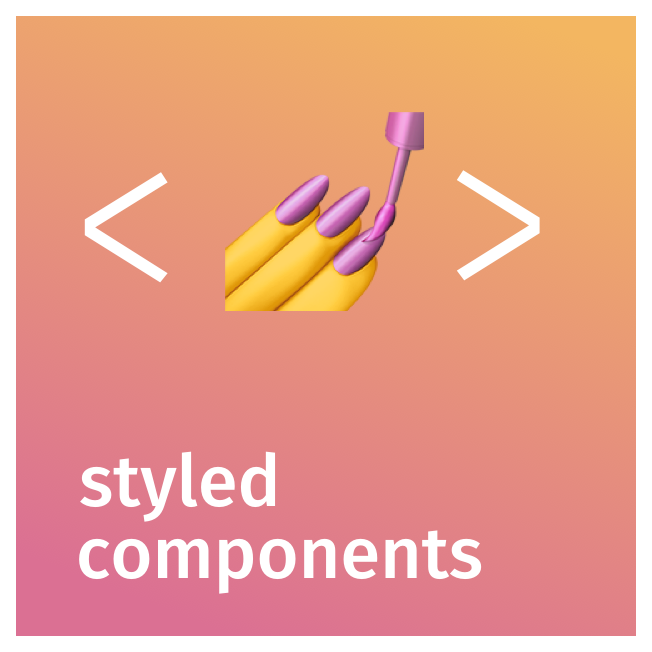
\includegraphics[height=2cm]{images/logos/styledComponent.png}
%     \caption{Logo de Styled Components}
% \end{figure}

\subsection*{TypeScript}
TypeScript est un langage de programmation open source qui étend la syntaxe de JavaScript en y ajoutant des fonctionnalités de typage statique. Il offre ainsi la possibilité de définir des types pour les variables, les paramètres de fonction, les objets et les valeurs de retour. Cette approche permet de détecter et de prévenir les erreurs de typage lors de la phase de développement, améliorant ainsi la robustesse et la qualité du code.
% \begin{figure}[!ht]
%     \centering %
%         
\includegraphics[height=2cm]{images/logos/typescript.png}
%     \caption{Logo de TypeScript}
% \end{figure}

\subsection*{Lerna}
Lerna est un outil open source qui facilite la gestion de projets monorepo, c'est-à-dire des projets qui contiennent plusieurs packages ou modules dans un même référentiel de code. Lerna permet de gérer ces packages de manière efficace en automatisant les tâches répétitives telles que l'installation des dépendances, la publication des packages, la gestion des versions, etc.\\

Avec Lerna, il est possible de partager du code entre différents packages, ce qui favorise la réutilisation et la modularité. Il permet également d'effectuer des tests et des déploiements cohérents sur l'ensemble des packages du monorepo.
% \begin{figure}[!ht]
%     \centering %
%         
\includegraphics[height=2cm]{images/logos/lerna.png}
%     \caption{Logo de Lerna}
% \end{figure}

\subsection*{Visual Studio Code}
Visual Studio Code est un éditeur de code extensible développé par Microsoft pour
Windows, Linux et macOS. Les fonctionnalités incluent la prise en charge du débogage,
la mise en évidence de la syntaxe, la complétion intelligente du code, les snippets, la
refactorisation du code et Git intégrer.
% \begin{figure}[!ht]
%     \centering %
%         
\includegraphics[height=2cm]{images/logos/vscode.jpeg}
%     \caption{Logo de Visual Studio Code}
% \end{figure}

\subsection*{IntelliJ IDEA}
IntelliJ IDEA, un environnement de développement intégré (IDE) puissant et polyvalent. IntelliJ IDEA est largement utilisé par les développeurs pour la programmation Java, mais il prend également en charge d'autres langages de programmation tels que JavaScript, TypeScript, Kotlin et bien d'autres.\\

IntelliJ IDEA offre une multitude de fonctionnalités pour améliorer la productivité des développeurs, telles que l'achèvement intelligent du code, la refactoring automatisé, la détection des erreurs en temps réel, la navigation avancée dans le code et bien d'autres. Il fournit également une intégration transparente avec les outils de gestion de version tels que Git, facilitant ainsi le suivi des modifications et la collaboration entre les membres de l'équipe.
% \begin{figure}[!ht]
%     \centering %
%         
\includegraphics[height=2cm]{images/logos/intellij logo.jpg}
%     \caption{Logo de IntelliJ}
% \end{figure}

\subsection*{Gradle}
\par Gradle est un moteur de production fonctionnant sur la plateforme Java. Il permet de construire des projets en Java, Scala, Groovy voire C++.

% \begin{figure}[!ht]
%     \centering %
%         
\includegraphics[height=2cm]{images/logos/gradle logo.png}
%     \caption{Logo de Gradle}
% \end{figure}

\par \textbf{Concepts de Gradle}
\begin{itemize}
\item  \textbf{Projets :}
Un projet représente une chose à faire, comme le déploiement d'applications dans des environnements de test. Un projet Gradle nécessite l'exécution d'un ensemble de tâches.

\item \textbf{Tâches :}
Une tâche fait référence à un travail effectué par un build. Cela peut être quelque chose d'aussi simple que compiler des classes, créer des fichiers JAR, créer Javadoc ou publier des archives.

\item  \textbf{Créer des scripts :}
Un script de construction est appelé build.gradle et se trouve dans le répertoire racine du projet. Chaque construction Gradle comprend un ou plusieurs projets.
\end{itemize}

\par \textbf{Fonctionnalités de Gradle}
\begin{itemize}
\item  \textbf{haute performance :}
Gradle termine rapidement la tâche en considérant les résultats des exécutions précédentes. Les travaux dont les entrées sont modifiées sont les seuls qui sont exécutés. Cela permet d'éviter les tâches inutiles et d'obtenir de meilleures performances.

\item  \textbf{Soutien :}
Connu pour fournir une assistance, nous utilisons Gradle pour les projets de construction ANT. Les tâches peuvent être importées depuis des projets de build ANT et peuvent être réutilisées dans Gradle. Il prend également en charge les dépôts Maven qui sont conçus pour publier et récupérer les dépendances du projet.

\item  \textbf{Construction de logiciel multi-projets :}
Gradle assure une prise en charge magnifique des builds multi-projets. Ces projets peuvent contenir un projet racine et un nombre illimité de sous-projets. Il prend en charge les constructions partielles, ce qui indique que l'outil déterminera si un projet dont notre projet dépend, a besoin d'un type de reconstruction. Au cas où le projet aurait besoin d'être reconstruit, Gradle le fera avant de construire d'autres projets.
\end{itemize}


\subsection*{Java}
Java est un langage populaire et largement utilisé dans le développement logiciel, notamment pour la création d'applications d'entreprise, de systèmes embarqués, de solutions web et bien plus encore.\\

Java offre de nombreux avantages, notamment sa portabilité, sa performance, sa sécurité et sa richesse en bibliothèques et frameworks. Il permet de développer des applications robustes et évolutives, en offrant une syntaxe claire et une structure orientée objet.

% \begin{figure}[!ht]
%     \centering %
%         
\includegraphics[height=2cm]{images/logos/java logo.png}
%     \caption{Logo de Java}
% \end{figure}

\subsection*{Java EE}
Java EE est une plateforme de développement d'applications d'entreprise qui fournit un ensemble de spécifications et de bibliothèques pour faciliter la création d'applications d'entreprise évolutives, robustes et sécurisées.\\

Java EE offre de nombreuses fonctionnalités et services essentiels pour le développement d'applications d'entreprise, tels que la gestion des transactions, la sécurité, la persistance des données, la gestion des ressources, la communication entre les composants et bien plus encore. Ces fonctionnalités intégrées permettent aux développeurs de se concentrer sur la logique métier de leur application, tout en bénéficiant d'une infrastructure solide et bien testée.
% \begin{figure}[!ht]
%     \centering %
%         
\includegraphics[height=2cm]{images/logos/java ee logo.png}
%     \caption{Logo de Java EE}
% \end{figure}

\subsection*{Spring}
Spring est un framework de développement d'applications Java qui offre une approche complète et modulaire pour la création d'applications d'entreprise.\\

Spring offre de nombreux modules et fonctionnalités qui facilitent le développement, tels que l'inversion de contrôle (IoC), la gestion des dépendances, la sécurité, la gestion des transactions, l'accès aux données, le développement web, et bien plus encore. Il favorise une architecture de développement propre et modulaire, permettant aux développeurs de se concentrer sur la logique métier de leur application sans se soucier des aspects techniques sous-jacents.
% \begin{figure}[!ht]
%     \centering %
%         
\includegraphics[height=2cm]{images/logos/spring logo.png}
%     \caption{Logo de Spring}
% \end{figure}

\subsection*{Sprign Boot}
Spring Boot est un framework basé sur Spring qui simplifie considérablement le processus de création d'applications Java autonomes et prêtes à l'emploi.\\

Spring Boot facilite la configuration et le déploiement de l'application en fournissant des conventions par défaut et en minimisant la configuration manuelle. Il offre également une intégration transparente avec d'autres technologies et frameworks, ce qui permet de développer rapidement des applications robustes.
% \begin{figure}[!ht]
%     \centering %
%         
\includegraphics[height=2cm]{images/logos/spring boot logo.png}
%     \caption{Logo de Spring Boot}
% \end{figure}

\subsection*{Sprign Security}
Spring Security est un framework puissant qui fournit des fonctionnalités de sécurité avancées pour les applications Java.\\

Avec Spring Security, nous avons pu mettre en place une authentification et une autorisation robustes pour nos utilisateurs. Nous avons utilisé différents mécanismes d'authentification, tels que l'authentification basée sur des formulaires, l'authentification basée sur des jetons, ainsi que l'intégration avec des fournisseurs d'authentification externes tels que OAuth.
% \begin{figure}[!ht]
%     \centering %
%         
\includegraphics[height=2cm]{images/logos/spring boot logo.png}
%     \caption{Logo de Spring Boot}
% \end{figure}


\subsection*{Pebble}
Pebble est un moteur de templates Java léger et puissant qui facilite la création de vues dynamiques et réutilisables.\\

Grâce à Pebble, nous avons pu séparer la logique métier de la présentation en utilisant des templates. Les templates Pebble sont écrits en utilisant une syntaxe simple et intuitive, ce qui nous a permis de créer rapidement des vues attrayantes et réactives pour notre application.

% \begin{figure}[!ht]
%     \centering %
%         
\includegraphics[height=2cm]{images/logos/pebble logo.png}
%     \caption{Logo de Pebble}
% \end{figure}

\subsection*{Jolt}
Jolt est un outil puissant qui nous a permis de structurer et de manipuler facilement des données JSON complexes.\\

Avec Jolt, nous avons pu définir des spécifications de transformation JSON en utilisant un langage de configuration simple et concis. Ces spécifications décrivent les modifications souhaitées dans la structure et les valeurs des données JSON, permettant ainsi de les transformer selon nos besoins.

% \begin{figure}[!ht]
%     \centering %
%         
\includegraphics[height=2cm]{images/logos/jolt_logo.png}
%     \caption{Logo de Jolt}
% \end{figure}

\subsection*{GraphQL}
GraphQL est un langage de requête et une technologie de communication de données qui offre une approche flexible et efficace pour récupérer et manipuler des données. Dans notre projet, nous avons utilisé GraphQL pour mettre en place une API de données robuste et personnalisable.\\

Avec GraphQL, nous avons pu définir un schéma de données qui décrit les types et les relations entre les données. Ce schéma agit comme un contrat entre le client et le serveur, permettant au client de spécifier exactement les données dont il a besoin et de les récupérer en une seule requête. Cela évite les problèmes de surcharge de données et d'appels multiples à l'API, améliorant ainsi les performances et l'efficacité.
% \begin{figure}[!ht]
%     \centering %
%         
\includegraphics[height=2cm]{images/logos/graphql logo.png}
%     \caption{Logo de GraphQL}
% \end{figure}

\subsection*{JUnit}
JUnit est un framework de test unitaire pour le langage de programmation Java. Dans notre projet, nous avons utilisé JUnit pour effectuer des tests unitaires afin de vérifier le bon fonctionnement de nos classes et méthodes individuelles.\\

JUnit offre une structure de test simple et efficace, permettant aux développeurs de définir des cas de test et d'exécuter automatiquement ces tests. Il fournit des assertions pour vérifier les résultats attendus des différentes opérations, ce qui facilite la détection des erreurs et des bugs.
% \begin{figure}[!ht]
%     \centering %
%         
\includegraphics[height=2cm]{images/logos/junit logo.png}
%     \caption{Logo de JUnit}
% \end{figure}


\subsection{Outils de documentation}
\subsection*{Storybook}
Storybook est un outil de développement interactif et de documentation qui facilite la création,
le test et la documentation des composants d’interface utilisateur. Il permet aux développeurs
de concevoir et de visualiser les composants de manière isolée, ce qui facilite l’exploration et la
validation des différentes configurations. Grâce à son interface intuitive, Storybook simplifie le
processus de développement et de débogage des composants. Il favorise également la collaboration
en permettant le partage des composants et la génération automatique de documentation. En
résumé, Storybook améliore l’efficacité du développement en offrant un environnement interactif
pour le développement et la documentation des composants d’interface utilisateur.
% \begin{figure}[!ht]
%     \centering %
%         
\includegraphics[height=2cm]{images/logos/storyboojk.png}
%     \caption{Logo de Storybook}
% \end{figure}

\subsection*{Swagger}
Swagger est un ensemble d'outils open-source permettant de concevoir, de construire, de documenter et de consommer des API RESTful. Il offre une approche basée sur la spécification, ce qui permet de décrire l'ensemble des fonctionnalités d'une API de manière standardisée et compréhensible par les développeurs et les utilisateurs.\\

Le cœur de Swagger est la spécification OpenAPI, anciennement connue sous le nom de Swagger Specification. Cette spécification utilise le format JSON ou YAML pour décrire les endpoints, les paramètres, les réponses et d'autres éléments clés d'une API. Grâce à cette spécification, il devient possible de générer automatiquement de la documentation interactive, des SDKs clients, des tests automatisés et d'autres artefacts liés à l'API.
% \begin{figure}[!ht]
%     \centering %
%         
\includegraphics[height=2cm]{images/logos/swagger.png}
%     \caption{Logo de Swagger}
% \end{figure}


\subsection{Outils de Test}
\subsection*{Cypress}
Cypress est un outil de test d'interface utilisateur open source, utilisé pour effectuer des tests end-to-end sur des applications web. Il offre une approche moderne et efficace pour écrire et exécuter des tests fonctionnels, intégration et de bout en bout.\\

Cypress se distingue par sa simplicité d'utilisation et sa capacité à exécuter les tests directement dans le navigateur. Il permet aux développeurs d'écrire des tests en utilisant une syntaxe JavaScript familière, et offre une interface de test interactive qui facilite le débogage et l'inspection des éléments de l'application.
% \begin{figure}[!ht]
%     \centering %
%         \includegraphics[height=2cm]{images/logos/cypress.jpeg}
%     \caption{Logo de Cypress}
% \end{figure}

\subsection*{Postman}
Postman est un outil populaire utilisé pour tester et développer des API. Il offre une interface conviviale qui permet aux développeurs de créer, envoyer et analyser des requêtes HTTP à destination de différentes API.\\

Dans notre projet, nous avons utilisé Postman pour tester et valider nos API. Nous avons pu envoyer des requêtes GET, POST, PUT, DELETE, etc. vers nos points de terminaison d'API pour vérifier leur fonctionnement et leur conformité aux spécifications.
% \begin{figure}[!ht]
%     \centering %
%         \includegraphics[height=2cm]{images/logos/postmanLogo.png}
%     \caption{Logo de Postman}
% \end{figure}

\subsection*{SoapUI}
SOAPUI est un outil open-source utilisé pour tester les services Web basés sur le protocole SOAP (Simple Object Access Protocol). Il offre une interface conviviale permettant de créer, exécuter et analyser des tests automatisés pour les services Web.\\

Avec SOAPUI, les développeurs et les testeurs peuvent facilement créer des requêtes SOAP en spécifiant les paramètres et les en-têtes appropriés. Ils peuvent également configurer des assertions pour valider les réponses des services en vérifiant les valeurs, les codes de statut et d'autres critères prédéfinis.
% \begin{figure}[!ht]
%     \centering %
%         \includegraphics[height=2cm]{images/logos/soapui.png}
%     \caption{Logo de SoapUI}
% \end{figure}

\subsection*{Karate}
Karate est un framework open-source de test d'API qui prend en charge les tests automatisés de services Web REST et SOAP. Il offre une approche simple et expressive pour écrire des scénarios de test, en utilisant un langage de script spécifique à Karate basé sur le langage Gherkin.\\

Avec Karate, les développeurs et les testeurs peuvent définir des étapes de test déclaratives dans des fichiers de scénarios, en utilisant des mots-clés compréhensibles par les acteurs métier. Cela permet de créer des tests automatisés faciles à comprendre et à maintenir, sans nécessiter de connaissances approfondies en programmation.
% \begin{figure}[!ht]
%     \centering %
%         \includegraphics[height=2cm]{images/logos/karate logo.png}
%     \caption{Logo de Karate}
% \end{figure}

\subsection*{Gherkin}
Le langage Gherkin est un langage utilisé pour écrire des scénarios de tests automatisés, basés sur le comportement attendu du système. Il se distingue par sa lisibilité et sa simplicité, ce qui le rend accessible aux acteurs métier non techniques.\\

Gherkin est basé sur une syntaxe claire et structurée, utilisant des mots-clés spécifiques tels que "Given" (Étant donné), "When" (Quand), "Then" (Alors) et d'autres. Ces mots-clés permettent de décrire les différentes étapes d'un scénario et d'exprimer les attentes vis-à-vis du système.
% \begin{figure}[!ht]
%     \centering %
%         \includegraphics[height=2cm]{images/logos/gherkin.png}
%     \caption{Logo de Gherkin}
% \end{figure}


\subsection{Outils de Gestion de Version}
\subsection*{Github}
GitHub, en tant qu’outil essentiel dans le développement front-end, joue un rôle central dans la
gestion de version et la collaboration. Il permet un contrôle précis des modifications du code source,
des revues de code efficaces et une intégration fluide des fonctionnalités développées. GitHub assure
la qualité, la traçabilité et la cohérence du travail tout au long du projet.
% \begin{figure}[!ht]
%     \centering %
%         \includegraphics[height=2cm]{images/logos/github.png}
%     \caption{Logo de Github}
% \end{figure}

\subsection{Outils de DevOps}
\subsection*{Intégration continue}
\subsubsection*{Sonarqube}
Sonarqube enregistre les mesures de qualité dans une base de données et les présente dans un tableau de
bord. Il fournit des tendances et des indicateurs avancés. L’idée principale est de fournir à
chaque développeur les mesures de la qualité du code de leurs projets.
% \begin{figure}[!ht]
%     \centering %
%         \includegraphics[height=2cm]{images/logos/sonarqube_logo.jpg}
%     \caption{Logo de Sonarqube}
% \end{figure}

\subsubsection*{Bolt-CI}
Une solution interne qui se charge des builds et des tests et qui informe les développeurs de
l’état de leur travail par mail ou dans leur profil github à chaque commit, dans les 2 premières
minutes après avoir déposé le code dans le repository. Elle informe également les autres outils
des changements dans les repositories github.\\

Une solution interne qui se charge de l’automatisation des builds et des tests (principalement
les tests unitaires), et qui renvoie le feedback aux développeurs par mail et github, après chaque
pull request fusionée.
% \begin{figure}[!ht]
%     \centering %
%         \includegraphics[height=2cm]{images/logos/boltCI-logo.png}
%     \caption{Logo de Bolt-CI}
% \end{figure}


\subsection*{Livraison continue}
\subsubsection*{Jenkins}
Jenkins est un outil d’automatisation open-source écrit en Java avec des plugins construits pour
les besoins du livraison continue. Jenkins est utilisé pour builder et tester vos projets logiciels
en temps réel, ce qui permet aux développeurs d’intégrer plus facilement les modifications
apportées au projet et aux utilisateurs d’obtenir plus facilement une nouvelle version.
% \begin{figure}[!ht]
%     \centering %
%         \includegraphics[height=2cm]{images/logos/jenkins-logo.png}
%     \caption{Logo de Jenkins}
% \end{figure}


\subsubsection*{Nexus}
Ce gestionnaire de dépôt permet de stocker et de récupérer des artefacts de
build. Il s’agit d’une version privée similaire aux gestionnaires de dépôts publics
populaires comme Maven Central Repository et jcenter de Bintray, que tout le
monde peut utiliser pour récupérer les dépendances publiques pour un projet
Maven.
% \begin{figure}[!ht]
%     \centering %
%         \includegraphics[height=2cm]{images/logos/nexus-logo.png}
%     \caption{Logo de Nexus}
% \end{figure}

\subsection*{Déploiement}
\subsubsection*{Bolt}
Il s’agit d’un outil développé en interne et fonctionnant dans tous les nœuds des machines
virtuelles de notre infrastructure. Il fournit une interface de ligne de commande simple pour
déclencher l’exécution de divers types d’applications avec une syntaxe à la fois simple et puissante.
% \begin{figure}[!ht]
%     \centering %
%         \includegraphics[height=2cm]{images/logos/boltCI-logo.png}
%     \caption{Logo de Bolt}
% \end{figure}

\subsubsection*{Nomad}
HashiCorp Nomad est un gestionnaire de charge moderne et léger. Nomad est également
connu comme un moteur d’orchestration comme Kubernetes. HashiCorp Nomad permet à toute organisation de déployer et de gérer facilement ses applications. Il peut non seulement orchestrer des applications conteneurisées mais aussi des applications patrimoniales à l’aide d’un flux de travail unique et unifié. Nomad peut également exécuter des applications Docker, non conteneurisées, microservices et batch.
% \begin{figure}[!ht]
%     \centering %
%         \includegraphics[height=2cm]{images/logos/nomad-logo.png}
%     \caption{Logo de Nomad}
% \end{figure}

\subsubsection*{Consul}
Consul est solution utilisée pour configurer dynamiquement des applications, coordonner des services,
ou servir de back-end de données pour Vault, ainsi qu’une multitude d’autres utilisations.
% \begin{figure}[!ht]
%     \centering %
%         \includegraphics[height=2cm]{images/logos/consul-logo.png}
%     \caption{Logo de Consul}
% \end{figure}

\subsubsection*{Vault}
Vault est un système de gestion des secrets et du chiffrement. Un secret est toute chose
dont on souhaite contrôler strictement l’accès, comme les clés de chiffrement des API, les mots de passe ou les certificats. Vault fournit des services de cryptage qui sont contrôlés par des méthodes d’authentification et d’autorisation. À l’aide de l’interface utilisateur, de l’interface
CLI ou de l’API HTTP de Vault, l’accès aux secrets et à d’autres données sensibles peut être
stocké et géré en toute sécurité, rigoureusement contrôlé (restreint) et vérifiable.
% \begin{figure}[!ht]
%     \centering %
%         \includegraphics[height=2cm]{images/logos/vault-logo.png}
%     \caption{Logo de Vault}
% \end{figure}

\subsection{Outils de Routage}
\subsection*{VIP}
Une VIP \textbf{adresse IP virtuelle} (ou VIPA) est une adresse IP publique qui
peut être partagée par plusieurs appareils connectés. En interne, chaque appareil
possède une adresse IP locale unique, mais en externe, ils partagent tous la même
adresse IP.

\subsection*{Traefik}
Traefik est un reverse proxy/load balancer. en tant que reverse proxy Traefik facilite le déploiement de micro-services. Il nous fournit un point d’entrée commun
vers notre infrastructure et permet de suivre et de surveiller toutes les requêtes entrantes et sortantes, et en tant que load balancer traefik peut distribuer la charge
sur tous les instances de notre système.
% \begin{figure}[!ht]
%     \centering %
%         \includegraphics[height=2cm]{images/logos/traefik-logo.png}
%     \caption{Logo de Traefik}
% \end{figure}

\subsection{Outils de Monitoring}
\subsection*{Grafana}
Au sein de la DiFa, garantir la disponibilité des services informatique est primordiale, pour cela l’équipe a pris une décision pour utiliser grafana comme étant un
outil de reporting, en effet grafana est une plateforme open source taillée pour
la surveillance, l’analyse et la visualisation des métriques. Elle est livrée avec un
serveur web (écrit en Go) permettant d’y accéder via une API HTTP.
% \begin{figure}[!ht]
%     \centering %
%         \includegraphics[height=2cm]{images/logos/grafana.jpg}
%     \caption{Logo de Grafana}
% \end{figure}

\subsection*{Kibana}
Pour mettre les logs visible est simple a comprendre, la DiFa a decidé d’utiliser
Kibana qui est est une application frontend gratuite et ouverte qui s’appuie sur la
Suite Elastic. Elle permet de rechercher et de visualiser les données indexées dans
Elasticsearch.Elle sert aussi d’interface utilisateur pour le monitoring, la gestion
et la sécurité des clusters de la Suite Elastic.
% \begin{figure}[!ht]
%     \centering %
%         \includegraphics[height=2cm]{images/logos/kibana.png}
%     \caption{Logo de Kibana}
% \end{figure}

\section{Interfaces}
Dans cette section consacrée à l'interface de notre application de banque en ligne, nous présentons les différentes pages et fonctionnalités qui permettent aux utilisateurs de gérer leurs comptes bancaires de manière pratique et personnalisée. Nous avons développé des interfaces adaptées à différents types d'appareils, notamment le bureau, la tablette et le mobile, afin d'offrir une expérience utilisateur optimale sur chaque plateforme.\\

Nous avons pris en compte les préférences linguistiques des utilisateurs en proposant des versions de langue en français et en anglais pour toutes les interfaces. Cela permet aux utilisateurs de choisir la langue qui leur convient le mieux, facilitant ainsi leur compréhension et leur interaction avec l'application, quel que soit leur pays ou leur langue préférée.
\subsection{Accueil}
Cette page constitue le point d'entrée principal pour les utilisateurs et offre une expérience conviviale et intuitive. Elle propose plusieurs options et fonctionnalités pour répondre aux besoins des utilisateurs.\\

Sur la page d'accueil, les utilisateurs ont la possibilité de choisir parmi différentes actions, telles que se connecter à leur compte, s'inscrire en tant que nouveau client, accéder au mode démonstration pour découvrir les fonctionnalités de l'application, utiliser le simulateur de crédit pour estimer les possibilités de financement, consulter les questions fréquentes pour obtenir des réponses aux interrogations courantes, trouver une agence bancaire à proximité, consulter les taux de change actuels et contacter notre équipe d'assistance via le formulaire de contact.
\begin{figure}[!ht]
    \centering
    \begin{subfigure}[b]{0.49\textwidth}
        \centering
        \includegraphics[width=\textwidth]{images/screens/accueil/desktop.png}
        \caption{version française}
    \end{subfigure}
    \hfill
    \begin{subfigure}[b]{0.49\textwidth}
        \centering
        \includegraphics[width=\textwidth]{images/screens/home/desktop.png}
        \caption{version anglaise}
    \end{subfigure}
       \caption{Interface Accueil sur le bureau}
\end{figure}

\newpage

\begin{figure}[!h]
    \centering
    \begin{subfigure}[b]{0.49\textwidth}
        \centering
        \includegraphics[width=\textwidth]{images/screens/accueil/tablette.png}
        \caption{version française}
    \end{subfigure}
    \hfill
    \begin{subfigure}[b]{0.49\textwidth}
        \centering
        \includegraphics[width=\textwidth]{images/screens/home/tablette.png}
        \caption{version anglaise}
    \end{subfigure}
       \caption{Interface Accueil sur la tablette}
\end{figure}

\newpage

\begin{figure}[!ht]
    \centering
    \begin{subfigure}[b]{0.49\textwidth}
        \centering
        \includegraphics[width=\textwidth]{images/screens/accueil/mob.png}
        \caption{version française}
    \end{subfigure}
    \hfill
    \begin{subfigure}[b]{0.49\textwidth}
        \centering
        \includegraphics[width=\textwidth]{images/screens/home/mob.png}
        \caption{version anglaise}
    \end{subfigure}
       \caption{Interface Accueil sur le mobile}
\end{figure}

\newpage

\subsection{Changement de langue}
Ce bouton permet aux utilisateurs de sélectionner la langue de leur choix pour afficher le contenu de l'application dans cette langue spécifique. Lorsque l'utilisateur clique sur le bouton de changement de langue, une alerte s'affiche avec deux options : confirmation et annulation.\\

Si l'utilisateur choisit de confirmer le changement de langue, l'application effectue le changement et redirige l'utilisateur vers la page d'accueil dans la nouvelle langue sélectionnée. Cela lui permet de bénéficier d'une expérience utilisateur dans la langue de son choix.\\

D'autre part, si l'utilisateur choisit d'annuler le changement de langue, aucun changement ne sera effectué et il restera sur la même page dans la langue actuelle.
\begin{figure}[!ht]
    \centering %
        \includegraphics[width=16cm]{images/screens/switch/desktop-switch.png}
    \caption{Bouton de changement de langue}
\end{figure}

\begin{figure}[!ht]
    \centering
    \begin{subfigure}[b]{0.49\textwidth}
        \centering
        \includegraphics[width=\textwidth]{images/screens/switch/desktop-fr.png}
        \caption{version française}
    \end{subfigure}
    \hfill
    \begin{subfigure}[b]{0.49\textwidth}
        \centering
        \includegraphics[width=\textwidth]{images/screens/switch/desktop-ang.png}
        \caption{version anglaise}
    \end{subfigure}
       \caption{Alerte de changement de langue sur le bureau et la tablette}
\end{figure}
\newpage

\begin{figure}[!ht]
    \centering
    \begin{subfigure}[b]{0.49\textwidth}
        \centering
        \includegraphics[width=\textwidth]{images/screens/switch/mob-fr.png}
        \caption{version française}
    \end{subfigure}
    \hfill
    \begin{subfigure}[b]{0.49\textwidth}
        \centering
        \includegraphics[width=\textwidth]{images/screens/switch/mob-ang.png}
        \caption{version anglaise}
    \end{subfigure}
       \caption{Alerte de changement de langue sur le mobile}
\end{figure}

\subsection{Mes Cartes}
L'interface "Mes cartes" offre une présentation claire et organisée des cartes monétiques, en fournissant des informations détaillées telles que le type de carte, le numéro de carte et la date d'expiration. Les utilisateurs peuvent également accéder à l'historique complet des transactions effectuées avec chaque carte, leur permettant ainsi de suivre leurs dépenses et de détecter les transactions suspectes. Cette interface utilise les API \textbf{getCards} et \textbf{getCardTransactions} pour récupérer les données nécessaires.
\begin{figure}[!ht]
    \centering
    \begin{subfigure}[b]{0.49\textwidth}
        \centering
        \includegraphics[width=\textwidth]{images/screens/cartes/desktop.png}
        \caption{version française}
    \end{subfigure}
    \hfill
    \begin{subfigure}[b]{0.49\textwidth}
        \centering
        \includegraphics[width=\textwidth]{images/screens/cards/desktop.png}
        \caption{version anglaise}
    \end{subfigure}
       \caption{Interface Mes cartes sur le bureau}
\end{figure}

\newpage

\begin{figure}[!ht]
    \centering
    \begin{subfigure}[b]{0.49\textwidth}
        \centering
        \includegraphics[width=\textwidth]{images/screens/cartes/tablette.png}
        \caption{version française}
    \end{subfigure}
    \hfill
    \begin{subfigure}[b]{0.49\textwidth}
        \centering
        \includegraphics[width=\textwidth]{images/screens/cards/tablette.png}
        \caption{version anglaise}
    \end{subfigure}
       \caption{Interface Mes cartes sur la tablette}
\end{figure}

\newpage


\begin{figure}[!ht]
    \centering
    \begin{subfigure}[b]{0.49\textwidth}
        \centering
        \includegraphics[width=\textwidth]{images/screens/cartes/mob.png}
        \caption{version française}
    \end{subfigure}
    \hfill
    \begin{subfigure}[b]{0.49\textwidth}
        \centering
        \includegraphics[width=\textwidth]{images/screens/cards/mob.png}
        \caption{version anglaise}
    \end{subfigure}
       \caption{Interface Mes cartes sur le mobile}
\end{figure}

\newpage

\begin{figure}[!ht]
    \centering
    \begin{subfigure}[b]{0.49\textwidth}
        \centering
        \includegraphics[width=\textwidth]{images/screens/mobileApp/device/Cards Home D.png}
    \end{subfigure}
    \hfill
    \begin{subfigure}[b]{0.49\textwidth}
        \centering
        \includegraphics[width=\textwidth]{images/screens/mobileApp/device/Cards Details D.png}
    \end{subfigure}
       \caption{Interface Mes cartes sur l'application mobile}
\end{figure}

\newpage

\begin{figure}[!ht]
    \centering
    \begin{subfigure}[b]{0.49\textwidth}
        \centering
        \includegraphics[width=\textwidth]{images/screens/cartes/mob-button.png}
        \caption{version française}
    \end{subfigure}
    \hfill
    \begin{subfigure}[b]{0.49\textwidth}
        \centering
        \includegraphics[width=\textwidth]{images/screens/cards/mob-button.png}
        \caption{version anglaise}
    \end{subfigure}
       \caption{Bouton pour voir plus de détails sur la transaction}
\end{figure}

\newpage

\begin{figure}[!ht]
    \centering
    \begin{subfigure}[b]{0.49\textwidth}
        \centering
        \includegraphics[width=\textwidth]{images/screens/cartes/mob-details.png}
        \caption{version française}
    \end{subfigure}
    \hfill
    \begin{subfigure}[b]{0.49\textwidth}
        \centering
        \includegraphics[width=\textwidth]{images/screens/cards/mob-details.png}
        \caption{version anglaise}
    \end{subfigure}
       \caption{Détails de la transaction}
\end{figure}

\newpage

\begin{figure}[!ht]
    \centering
    \begin{subfigure}[b]{0.49\textwidth}
        \centering
        \includegraphics[width=\textwidth]{images/screens/mobileApp/device/Cards Transactions Details D.png}
    \end{subfigure}
       \caption{Détails de la transaction dans l'application mobile}
\end{figure}

\subsection{Plafonds des cartes}
L'interface "Plafonds des cartes" offre une vue claire et détaillée des limites nationales et internationales de chaque carte.\\

Grâce à l'API \textbf{getCardLimits}, les données sont récupérées en temps réel pour assurer que les informations affichées sont toujours à jour.
\newpage
\subsubsection*{Plafonds nationaux}
\begin{figure}[!ht]
    \centering
    \begin{subfigure}[b]{0.49\textwidth}
        \centering
        \includegraphics[width=\textwidth]{images/screens/plafondsNat/desktop.png}
        \caption{version française}
    \end{subfigure}
    \hfill
    \begin{subfigure}[b]{0.49\textwidth}
        \centering
        \includegraphics[width=\textwidth]{images/screens/limitsnat/desktop.png}
        \caption{version anglaise}
    \end{subfigure}
       \caption{Interface Plafonds nationaux sur le bureau}
\end{figure}

\begin{figure}[!ht]
    \centering
    \begin{subfigure}[b]{0.49\textwidth}
        \centering
        \includegraphics[width=\textwidth]{images/screens/plafondsNat/tablette.png}
        \caption{version française}
    \end{subfigure}
    \hfill
    \begin{subfigure}[b]{0.49\textwidth}
        \centering
        \includegraphics[width=\textwidth]{images/screens/limitsnat/tablette.png}
        \caption{version anglaise}
    \end{subfigure}
       \caption{Interface Plafonds nationaux sur la tablette}
\end{figure}

\newpage

\begin{figure}[!ht]
    \centering
    \begin{subfigure}[b]{0.49\textwidth}
        \centering
        \includegraphics[width=\textwidth]{images/screens/plafondsNat/mob.png}
        \caption{version française}
    \end{subfigure}
    \hfill
    \begin{subfigure}[b]{0.49\textwidth}
        \centering
        \includegraphics[width=\textwidth]{images/screens/limitsnat/mob.png}
        \caption{version anglaise}
    \end{subfigure}
       \caption{Interface Plafonds nationaux sur le mobile}
\end{figure}
\newpage

\begin{figure}[!ht]
    \centering
    \begin{subfigure}[b]{0.49\textwidth}
        \centering
        \includegraphics[width=\textwidth]{images/screens/mobileApp/device/Cards Limits D.png}
    \end{subfigure}
    \begin{subfigure}[b]{0.49\textwidth}
        \centering
        \includegraphics[width=\textwidth]{images/screens/mobileApp/device/Cards Limits Details D.png}
    \end{subfigure}
       \caption{Interface Plafonds nationaux sur l'application mobile}
\end{figure}

\newpage

\subsubsection*{Plafonds internationaux}
\begin{figure}[!ht]
    \centering
    \begin{subfigure}[b]{0.49\textwidth}
        \centering
        \includegraphics[width=\textwidth]{images/screens/plafondsInter/desktop.png}
        \caption{version française}
    \end{subfigure}
    \hfill
    \begin{subfigure}[b]{0.49\textwidth}
        \centering
        \includegraphics[width=\textwidth]{images/screens/limitsInter/desktop.png}
        \caption{version anglaise}
    \end{subfigure}
       \caption{Interface Plafonds internationaux sur le bureau}
\end{figure}

\begin{figure}[!ht]
    \centering
    \begin{subfigure}[b]{0.49\textwidth}
        \centering
        \includegraphics[width=\textwidth]{images/screens/plafondsInter/tablette.png}
        \caption{version française}
    \end{subfigure}
    \hfill
    \begin{subfigure}[b]{0.49\textwidth}
        \centering
        \includegraphics[width=\textwidth]{images/screens/limitsInter/tablette.png}
        \caption{version anglaise}
    \end{subfigure}
       \caption{Interface Plafonds internationaux sur la tablette}
\end{figure}
\newpage

\begin{figure}[!ht]
    \centering
    \begin{subfigure}[b]{0.49\textwidth}
        \centering
        \includegraphics[width=\textwidth]{images/screens/plafondsInter/mob.png}
        \caption{version française}
    \end{subfigure}
    \hfill
    \begin{subfigure}[b]{0.49\textwidth}
        \centering
        \includegraphics[width=\textwidth]{images/screens/limitsInter/mob.png}
        \caption{version anglaise}
    \end{subfigure}
       \caption{Interface Plafonds internationaux sur le mobile}
\end{figure}
% \newpage

\subsection{Mes Produits}
L'interface "Mes produits" permet aux utilisateurs de consulter les différents produits bancaires souscrits pour un compte spécifique. Cette fonctionnalité offre une vue d'ensemble complète des engagements financiers associés à chaque compte, tels que les crédits, les prêts ou les services d'investissement.\\

Grâce à l'API \textbf{getAccountProducts}, les données sont récupérées en temps réel pour assurer que les informations affichées sont toujours à jour. Les utilisateurs peuvent visualiser les détails de chaque produit, y compris les caractéristiques, les conditions d'utilisation et les dates d'échéance.

\begin{figure}[!ht]
    \centering
    \begin{subfigure}[b]{0.49\textwidth}
        \centering
        \includegraphics[width=\textwidth]{images/screens/produits/desktop.png}
        \caption{version française}
    \end{subfigure}
    \hfill
    \begin{subfigure}[b]{0.49\textwidth}
        \centering
        \includegraphics[width=\textwidth]{images/screens/products/desktop.png}
        \caption{version anglaise}
    \end{subfigure}
       \caption{Interface Mes produits sur le bureau}
\end{figure}
\newpage

\begin{figure}[!ht]
    \centering
    \begin{subfigure}[b]{0.49\textwidth}
        \centering
        \includegraphics[width=\textwidth]{images/screens/produits/tablette.png}
        \caption{version française}
    \end{subfigure}
    \hfill
    \begin{subfigure}[b]{0.49\textwidth}
        \centering
        \includegraphics[width=\textwidth]{images/screens/products/tablette.png}
        \caption{version anglaise}
    \end{subfigure}
       \caption{Interface Mes produits sur la tablette}
\end{figure}
\newpage

\begin{figure}[!ht]
    \centering
    \begin{subfigure}[b]{0.49\textwidth}
        \centering
        \includegraphics[width=\textwidth]{images/screens/produits/mob.png}
        \caption{version française}
    \end{subfigure}
    \hfill
    \begin{subfigure}[b]{0.49\textwidth}
        \centering
        \includegraphics[width=\textwidth]{images/screens/products/mob.png}
        \caption{version anglaise}
    \end{subfigure}
       \caption{Interface Mes produits sur le mobile}
\end{figure}


\subsection{Téléchargement du récapitulatif}
Les utilisateurs ont la possibilité de télécharger le récapitulatif d'un produit spécifique auquel ils ont souscrit. Pour ce faire, il leur suffit de cliquer sur le bouton "Télécharger le récapitulatif" associé au produit concerné.\\

\begin{figure}[!ht]
    \centering %
        \includegraphics[width=16cm]{images/screens/produits/desktop-button.png}
    \caption{Bouton de téléchargement du récapitulatif}
\end{figure}

Lorsque l'utilisateur clique sur ce bouton, notre application génère automatiquement le récapitulatif du produit souscrit et le propose en téléchargement. Le fichier téléchargé contient toutes les informations pertinentes sur le produit, telles que les détails de souscription, les termes et conditions, les fonctionnalités, et tout autre élément pertinent lié au produit.
\begin{figure}[!ht]
    \centering %
        \includegraphics[width=16cm]{images/screens/produits/Récapitulatif.png}
    \caption{Exemple d'un récapitulatif de produit}
\end{figure}
\newpage

\section{Environnements de déploiement}
Les stratégies de déploiement suivies dans notre projet sont différentes selon l’environnement de
déploiement. Les environnements adoptés par la DIFA sont :

\begin{itemize}
    \item[•] \textbf{LOCAL :} L’environnement LOCAL est utilisé par les développeurs sur leurs propres machines
    pour le développement et les tests. Ils disposent d’une installation locale du système et des outils
    nécessaires. Cela leur permet de travailler de manière autonome et de tester les fonctionnalités
    dans un environnement contrôlé.
    \item[•] \textbf{Development [DEV] :} Il s’agit du premier niveau de machines individuelles, à ce stade l’application est hébergée dans un ou plusieurs agents Nomad dans une ou plusieurs machines virtuelles
    fonctionnant dans des centres de données cloud privés, seuls les développeurs y ont accès pour
    valider la fonctionnalité de leur application lors de l’exécution.
    \item[•] \textbf{Homologation Fonctionnelle [HF] :} Tout comme le DEV, cet environnement est hébergée dans un agent Nomad avec des informations d’identification et des données stockées en toute sécurité,
    ces données diffèrent de celle de l’environnement DEV car elles doivent communiquer avec d’autres
    instances d’autres systèmes, cet environnement est créé pour que les Business Analyst, les Proxy
    Product Owner et les Product Owner puissent y exécuter les tests d’acceptation et valider le comportement de l’application.
    \item[•] \textbf{Homologation Technique [HT] :} Également appelé ISO-PROD, ce qui signifie qu’il a exactement les mêmes caractéristiques que l’environnement de production. Il permet de tester l’application dans un environnement de type production, et valider qu’elle supporte la charge de travail,
    les critères du système et tout incident technique pouvant survenir en production.
    \item[•] \textbf{Production [PROD] :}  A ce stade l’application est entièrement testée et validée pour être accessible aux clients, elle est également dupliquée dans plusieurs instances, différentes machines
    physiques, et aussi différentes régions géographiques pour assurer une disponibilité permanente
    possible.
\end{itemize}

\section{Qualification}
La phase de qualification comprend différents tests qui garantissent la qualité et la fiabilité du
système. Parmi ces tests, on retrouve les tests end-to-end, les tests fonctionnels et les tests de
non-régression.

\subsection{Tests end to end}
Les tests end-to-end, réalisés en environnement local sont réalisés pour vérifier le fonctionnement
global du système, en simulant des scénarios réels de bout en bout. Ils permettent de valider
l’intégration des différents composants et de s’assurer que toutes les fonctionnalités interagissent
correctement.
\begin{figure}[!h]
    \centering %
        \includegraphics[width=16cm]{images/realisation/cypressLanguage.png}
    \caption{Exemple de test end to end en utilisant Cypress}
\end{figure}
\newpage

\subsection{Tests fonctionnels}
Les tests fonctionnels, réalisés en environnement HF, se concentrent sur la vérification des fonctionnalités individuelles du système. Ils permettent de valider que chaque fonctionnalité répond
aux exigences spécifiées et fonctionne comme prévu.
\subsection{Tests de non regression}
Les tests de non-régression, réalisés en environnement HT, sont effectués pour s’assurer que les
modifications apportées au système n’ont pas introduit de régressions, c’est-à-dire qu’elles n’ont pas affecté négativement les fonctionnalités existantes. Ces tests garantissent la stabilité du système
lors de l’ajout de nouvelles fonctionnalités ou de modifications.

\section{Perspectives}  
Nous identifions plusieurs fonctionnalités qui peuvent être développées dans le cadre futur du projet de banque en ligne. Bien que ces fonctionnalités n'aient pas encore été implémentées, elles représentent des opportunités d'amélioration et d'extension du système. Les principales perspectives sont les suivantes :

\begin{itemize}
    \item[•] \textbf{Modification des plafonds :}  Une fonctionnalité clé à envisager est la possibilité pour les utilisateurs de modifier les plafonds de leurs cartes. Cela permettrait aux clients d'ajuster les limites de dépenses et de retraits en fonction de leurs besoins et de leurs préférences, offrant ainsi une plus grande flexibilité et un meilleur contrôle sur leurs transactions financières.
    \item[•] \textbf{Développement de la page "Store" :} Une autre perspective intéressante est la création d'une page dédiée au "Store" où les utilisateurs peuvent découvrir et consulter les produits financiers proposés par les banques partenaires. Cette fonctionnalité permettrait aux clients d'avoir une vision plus complète et transparente des offres disponibles, favorisant ainsi une prise de décision éclairée pour leurs besoins bancaires.
    \item[•] \textbf{Déploiement :}  Le déploiement est une étape essentielle pour rendre le système de banque en ligne accessible aux clients finaux. Cette perspective implique le déploiement de l'application sur des serveurs ou des infrastructures adaptés, permettant ainsi une utilisation réelle par les utilisateurs. Un déploiement réussi garantirait une disponibilité et une stabilité optimales de l'application pour une expérience utilisateur fluide et fiable.
\end{itemize}

\section{Conclusion}
Le chapitre "Réalisation et mise en œuvre" a été une étape clé dans notre projet de développement de la banque en ligne. Nous avons réussi à concrétiser les spécifications et les besoins identifiés lors de l'étude détaillée du projet, en mettant en place les interfaces, les fonctionnalités et les environnements nécessaires.

\addcontentsline{toc}{chapter}{Conclusion générale}
\chapter*{Conclusion générale}
Ce rapport de projet de fin d'études a présenté le développement d'une application de banque en ligne moderne et fonctionnelle. Nous avons commencé par une étude détaillée du projet, en spécifiant les besoins, en analysant les cas d'utilisation et en concevant l'architecture du système. Ensuite, nous avons passé à la phase de réalisation et de mise en œuvre, où nous avons utilisé divers outils et technologies pour développer les fonctionnalités de l'application. Nous avons également souligné l'importance des tests et de la qualification pour assurer la qualité et la fiabilité du système.\\

Ce projet nous a permis de mettre en pratique nos connaissances en développement web et mobile, en utilisant des technologies telles que React.js, React Native, Redux, TypeScript, et bien d'autres. Nous avons également pu acquérir de l'expérience dans la conception d'interfaces utilisateur attrayantes et conviviales, en utilisant des outils tels que Figma et Storybook.\\

Bien que notre application de banque en ligne soit fonctionnelle et offre des fonctionnalités clés, nous reconnaissons qu'il reste des perspectives d'amélioration et de développement futur. Certaines fonctionnalités, telles que la modification des plafonds et la création d'une page de boutique pour les produits bancaires, n'ont pas encore été développées. De plus, le déploiement de l'application dans des environnements réels nécessite une attention particulière pour assurer une disponibilité continue et une performance optimale.\\

En conclusion, ce projet de fin d'études nous a permis d'appliquer nos compétences techniques et de relever les défis de développement d'une application de banque en ligne complète. Nous avons acquis une expérience précieuse dans la conception, la réalisation et la mise en œuvre d'un système de ce type. Nous sommes fiers des résultats obtenus et nous sommes confiants que ce projet contribuera à notre développement professionnel. Nous tenons à remercier tous ceux qui ont contribué à la réussite de ce projet, y compris notre équipe, nos encadrants et tous les autres intervenants.

\newpage

%récupérer les citation avec "/footnotemark"
\nocite{*}

%choix du style de la biblio
\bibliographystyle{plain}
%inclusion de la biblio
\bibliography{bibliographie.bib}
%voir wiki pour plus d'information sur la syntaxe des entrées d'une bibliographie

\end{document}